%%%%%%%%%%%%%%%%%%%%%%%%
% Sample use of the infthesis class to prepare an MSc thesis.
% This can be used as a template to produce your own thesis.
% Date: June 2019
%
%
% The first line specifies style options for taught MSc.
% You should add a final option specifying your degree.
% *Do not* change or add any other options.
%
% So, pick one of the following:
% \documentclass[msc,deptreport,adi]{infthesis}     % Adv Design Inf
% \documentclass[msc,deptreport,ai]{infthesis}      % AI
% \documentclass[msc,deptreport,cogsci]{infthesis}  % Cognitive Sci
% \documentclass[msc,deptreport,cs]{infthesis}      % Computer Sci
% \documentclass[msc,deptreport,cyber]{infthesis}   % Cyber Sec
% \documentclass[msc,deptreport,datasci]{infthesis} % Data Sci
% \documentclass[msc,deptreport,di]{infthesis}      % Design Inf
% \documentclass[msc,deptreport,inf]{infthesis}     % Informatics
%%%%%%%%%%%%%%%%%%%%%%%%

\documentclass[msc,deptreport.inf]{infthesis} % Do not change except to add your degree (see above).

% maths
\usepackage{amsmath}
\usepackage{amsfonts}
\usepackage{amssymb}
\newcommand{\matr}[1]{\mathbf{#1}}
\newcommand{\bgreek}[1]{\boldsymbol{#1}}
\newcommand{\R}{\mathbb R}
\newcommand{\E}{\mathbb E}
\newcommand{\V}{\mathbb V}
\newcommand{\N}{\mathbb N}
\newcommand{\D}{\mathbb D}
\newcommand{\diag}{\mathop{\mathrm{diag}}}
\newcommand{\tr}{\mathop{\mathrm{Tr}}}

% algorithms
\usepackage{algorithm, algpseudocode}
\renewcommand{\algorithmicrequire}{\textbf{Input:}}
\renewcommand{\algorithmicensure}{\textbf{Output:}}

% graphics
\usepackage{graphicx}
\usepackage{subfig}


\begin{document}
\begin{preliminary}

\title{Fast and Scalable Factor Analysis Algorithms for Bayesian Deep Learning}

\author{Scott Brownlie}

\abstract{
%  This skeleton demonstrates how to use the \texttt{infthesis} style
%  for MSc dissertations in Artificial Intelligence, Cognitive Science,
%  Computer Science, Data Science, and Informatics. It also emphasises
%  the page limit, and that you must not deviate from the required
%  style.  The file \texttt{skeleton.tex} generates this document and
%  can be used as a starting point for your thesis. The abstract should
%  summarise your report and fit in the space on the first page.

Learning the posterior distribution of a deep neural network is a difficult task. Even when using a Gaussian approximation, one faces the daunting challenge of estimating the $D \times D$ posterior covariance matrix, where $D$, the number of model parameters, can reach billions by today's standards. Some simplification has to be made, and one option is to use a low-rank plus diagonal approximation. This approach is more flexible than a solely diagonal approximation, since it preserves some of the off-diagonal structure of the covariance matrix. 

One particular Gaussian distribution with a low-rank plus diagonal covariance matrix is the factor analysis model. In its essence, factor analysis is a latent variable model which generates observations via an affine transformation of the latents plus the addition of some Gaussian noise. This project makes use of these properties to derive novel algorithms for posterior estimation of deep neural networks. 

Two distinctly different approaches are considered. The first of these is inspired by a recent Bayesian deep learning method called SWAG.  It is based on the assumption that samples representative of the true posterior are encountered while training the neural network via stochastic gradient descent. Two algorithms are presented which learn factor analysis models from such samples in an online, iterative fashion, making them suitable for high-dimensional data, such as the parameters vector of a deep neural network. Experiments demonstrate that the algorithms are often as effective at learning factor analysis models as the classic batch algorithm based on singular value decomposition.

The second approach is based on variational inference and does not require a separate posterior sampling procedure. The algorithm - aptly named VIFA due to its use of variational inference and factor analysis - is model-agnostic and can be readily applied to any type of neural network architecture with no extra effort. Crucially, the implementation scales to very high-dimensional deep neural networks. Experiments demonstrate its effectiveness in learning the posterior and making predictions with uncertainty estimates, as well as its impressive speed compared to a recent method called SLANG with adopts a similar approach. 
}

\maketitle

\section*{Acknowledgements}
Any acknowledgements go here.

\tableofcontents
\end{preliminary}


\chapter{Introduction}

%The preliminary material of your report should contain:
%\begin{itemize}
%\item
%The title page.
%\item
%An abstract page.
%\item
%Optionally an acknowledgements page.
%\item
%The table of contents.
%\end{itemize}
%
%As in this example \texttt{skeleton.tex}, the above material should be
%included between:
%\begin{verbatim}
%\begin{preliminary}
%    ...
%\end{preliminary}
%\end{verbatim}
%This style file uses roman numeral page numbers for the preliminary material.
%
%The main content of the dissertation, starting with the first chapter,
%starts with page~1. \emph{\textbf{The main content must not go beyond page~40.}}
%
%The report then contains a bibliography and any appendices, which may go beyond
%page~40. The appendices are only for any supporting material that's important to
%go on record. However, you cannot assume markers of dissertations will read them.
%
%You may not change the dissertation format (e.g., reduce the font
%size, change the margins, or reduce the line spacing from the default
%1.5 spacing). Over length or incorrectly-formatted dissertations will
%not be accepted and you would have to modify your dissertation and
%resubmit.  You cannot assume we will check your submission before the
%final deadline and if it requires resubmission after the deadline to
%conform to the page and style requirements you will be subject to the
%usual late penalties based on your final submission time.

%\section{Using Sections}
%
%Divide your chapters into sub-parts as appropriate.
%
%\section{Citations}
%
%Citations (such as \cite{P1} or \cite{P2}) can be generated using
%\texttt{BibTeX}. For more advanced usage, the \texttt{natbib} package is
%recommended. You could also consider the newer \texttt{biblatex} system.
%
%These examples use a numerical citation style. You may also use
%(Author, Date) format if you prefer.
%
%\chapter{Your next chapter}
%
%A dissertation usually contains several chapters.

In recent years, deep learning \cite{goodfellow2016} has come to dominate many areas of machine learning. Deep learning models continue to achieve state of the art results in several domains, such as CoAtNet-7 \cite{dai2021} for image classification and Megatron-LM \cite{shoeybi2019} for language modelling. One reason for their success is the availability of huge training sets, such as the 300 millions images in JFT-300M \cite{sun2017} or the 100 million tokens in WikiText-103 \cite{merity2016}. The number of training examples, however, pales in comparison to the number of learnable parameters in some deep models. CoAtNet-7, for example, has 2.4 billion parameters, whereas Megatron-LM has a whopping 8.3 billion. This is a common feature of deep learning: the number of model parameters is often greater than the number of training examples. In this scenario, the model is severely \emph{underspecified} by the data and many different settings of the parameters are able to explain the training set equally well. In some domains, choosing a single setting of the parameters and predicting a point estimate for each test example is satisfactory. However, for other critical applications, some measure of the uncertainty in the prediction is also required. This is where Bayesian deep learning comes in. Instead of choosing a single parameter vector $\theta \in \R^D$ for the neural network, predictions are made using \emph{all} possible parameter vectors weighted by their posterior probabilities, given the training data $\mathcal{D}$. Formally, the posterior predictive distribution of the output $y$ given the input $\matr{x}$ is
\begin{equation}
	p(y | \matr{x}, \mathcal{D}) = \int p(y | \matr{x}, \theta) p(\bgreek{\theta} | \mathcal{D}) d\theta.
\end{equation}
In practice, computing this integral is intractable due to the dimensionality and non-linearities of a deep neural network. However, the integral can be approximated by a \emph{Bayesian model average},
\begin{equation}
	p(y | \matr{x}, \mathcal{D}) \approx \frac{1}{L} \sum_{l=1}^L p(y | \matr{x}, \theta_l), 
	\quad \theta_l \sim p(\bgreek{\theta} | \mathcal{D}).
\end{equation}
Note that this requires samples from the \emph{posterior}, $p(\bgreek{\theta} | \mathcal{D})$, which is defined as
\begin{equation}
	p(\bgreek{\theta} | \mathcal{D}) = \frac{p(\mathcal{D} | \theta) p(\theta)}{p(\mathcal{D})},
\end{equation}
where $p(\mathcal{D} | \theta)$ is the \emph{likelihood} that $\theta$ generated $\mathcal{D}$, $p(\theta)$ is the \emph{prior} and $p(\mathcal{D})$ is the \emph{marginal likelihood}. Unfortunately, this calculation is also intractable due to the high-dimensional integral $p(\mathcal{D}) = \int p(\mathcal{D} | \theta) p(\theta) d\theta$. A common alternative is to approximate $p(\bgreek{\theta} | \mathcal{D})$ with a Gaussian distribution with mean $\mu \in \R^D$ and covariance $\Sigma \in \R^{D\times D}$, denoted by $\mathcal{N}(\mu, \Sigma)$. The key practical challenge is then finding a way to approximate $\Sigma$, since the full $D\times D$ covariance matrix will not fit into memory for large $D$. 

One of the simplest approaches is to use a diagonal - or \emph{mean-field} - approximation \cite{blundell2015, graves2011, hernandez2015, tangkaratt2018, ranganath2014}. This is convenient in the sense that the covariance matrix is completely specified by $D$ parameters, but it does not allow for any posterior correlations between different elements of $\theta$. A more flexible approach is a low-rank plus diagonal approximation, $\matr{F}\matr{F}^\intercal + \Psi$, where $\matr{F} \in \R^{D\times K}$ and $\Psi$ is a $D \times D$ diagonal matrix. This preserves some of the off-diagonal structure of the covariance matrix and is practically feasible for $K \ll D$. Two recent methods which adopt this approach are SWAG \cite{maddox2019} and SLANG \cite{mishkin2018}. While both algorithms have achieved promising results, they also have fundamental limitations. In the case of SWAG, it does not make use of all the available data to fit the low-rank plus diagonal covariance matrix, whereas the current implementation of SLANG only supports fully-connected neural networks and would require non-trivial modifications for other types of architectures.

The work in this thesis is based on the low-rank plus diagonal factor analysis model, which can help to overcome these limitations. The main contributions are:
\begin{itemize}
	\item \textbf{two novel online algorithms for learning factor analysis models of high-dimensional data, which can be used in conjunction with SWAG};
	\item \textbf{a novel variational inference algorithm similar to SLANG, but which can be applied to any neural network architecture with no extra effort}. 
\end{itemize} 
Chapter \ref{ch:background} introduces the background required to follow the rest of the thesis. Chapter \ref{ch:previous_work} describes SWAG and SLANG in more detail and sets out the main goals that the thesis hopes to achieve. Chapter \ref{ch:online_fa} presents the online factor analysis algorithms and the results of applying them to synthetic datasets. Chapter \ref{ch:vifa} introduces VIFA, a novel variational inference algorithm, and demonstrates its effectiveness in estimating the posterior and making predictions. Finally, Chapter \ref{ch:conclusions} brings the thesis to an end with some conclusions and suggestions for future work. 


\chapter{Background}\label{ch:background}

This chapter presents the background necessary to understand the rest of the thesis. Bayesian linear regression, whose posterior can be computed in closed for, provides a nice testbed for the algorithms. Moreover, it can be viewed as a simple neural network with a single affine layer from input to output. Therefore, it is introduced first, followed by the general case of a neural network with multiple layers. The most common training algorithm for neural networks, stochastic gradient descent, is described next. Factor analysis is then introduced, as this is the basis of the main contributions in this thesis. Finally, variational inference is described as a pre-requisite for algorithms which use this approach to learn the posterior distribution of a neural network. 

\section{Bayesian Linear Regression}\label{sec:bayesian_lr}

A linear regression model is a mapping from vector inputs $\matr{x} \in \R^D$ to scalar outputs $y \in \R$ via an affine transformation. Given a set of observed input-output pairs, $\mathcal{D} = \{(\matr{x}_n, y_n)\}_{n=1}^{N}$, it is assumed that each output is generated according to 
\begin{equation}\label{eqn:linear_regression}
	y_n = \theta^\intercal \matr{x}_n + \epsilon_n
\end{equation}
for some unknown $\theta \in \R^D$. The underlying signal, $\theta^\intercal \matr{x}_n$, is corrupted by additive noise, 
\begin{equation}
	\epsilon_n \sim \mathcal{N}(0, \sigma^2), 
\end{equation}
for some $\sigma > 0$ \cite{barber2007}. The model is often written with an explicit bias term, but this can be absorbed into $\theta$ by adding a constant of one to the input, leading to the expression in Equation (\ref{eqn:linear_regression}). Due to the additive noise, each $y_n$ is a random variable, conditioned on $\matr{x}_n$ and $\theta$. Since $\epsilon_n$ is Gaussian distributed, the conditional pdf of $y_n$ is 
\begin{equation}\label{eqn:linear_regression_pdf}
	p(y_n | \theta, \matr{x}_n) 
	= \mathcal{N}\big(\theta^\intercal \matr{x}_n, \sigma^2\big)
	= \frac{1}{\sqrt{2\pi \sigma^2}} \exp\Big(-\frac{1}{2\sigma^2} \big(y_n - \theta^\intercal \matr{x}_n \big)^2\Big).
\end{equation}
Assuming that the observations in $\mathcal{D}$ are independent and identically distributed (iid), the log-likelihood of $\theta$ having generated the data is 
\begin{align}\label{eqn:linear_regression_log_likelihood}
\begin{split}
	\log p(\mathcal{D} | \theta) 
	& = \sum_{n=1}^N \big[ \log p(y_n | \theta, \matr{x}_n)  + \log p(\matr{x}_n) \big] \\
	& = \sum_{n=1}^N \Big[ -\frac{1}{2} \log 2\pi \sigma^2 - \frac{1}{2\sigma^2} \big(y_n - \theta^\intercal \matr{x}_n \big)^2 \Big]
	+ \sum_{n=1}^N \log p(\matr{x}_n) \\
	& = - \frac{1}{2 \sigma^2} \sum_{n=1}^N \big(y_n - \theta^\intercal \matr{x}_n \big)^2 
	- \frac{N}{2} \log \sigma^2
	- \frac{N}{2} \log 2\pi
	+ \sum_{n=1}^N \log p(\matr{x}_n) \\
	& = - \frac{\beta}{2} \sum_{n=1}^N \big(y_n - \theta^\intercal \matr{x}_n \big)^2 
	+ \frac{N}{2} \log \beta
	+ \text{constant},
\end{split}
\end{align}
where $\beta = \frac{1}{\sigma^2}$ is the \emph{noise precision} \cite{barber2007}. In Bayesian linear regression, a prior distribution for $\theta$ is also specified. A common choice  is 
\begin{equation}\label{eqn:linear_regression_prior}
	p(\theta) 
	= \mathcal{N}\big(\matr{0}, \alpha^{-1} \matr{I} \big)
	= \Big(\frac{\alpha}{2\pi}\Big)^{\frac{D}{2}} \exp\Big(-\frac{\alpha}{2} \theta^\intercal \theta \Big)
\end{equation}
for some $\alpha > 0$, which is a hyperparameter known as the \emph{prior precision} \cite{barber2007}. Given the log-likelihood and the prior, it turns out that the posterior distribution of $\theta$ is Gaussian and can be computed in closed form. Formally, 
\begin{equation}\label{eqn:linear_regression_posterior}
	p(\theta | \mathcal{D}) = \mathcal{N}(\matr{A}^{-1} \matr{b}, \matr{A}^{-1}),
\end{equation}
where
\begin{equation}\label{eqn:linear_model_A_and_b}
	\matr{A} = \alpha \matr{I} + \beta \sum_{n=1}^N \matr{x}_n \matr{x}_n^\intercal
	\quad \text{and} \quad 
	\matr{b} = \beta \sum_{n=1}^N y_n \matr{x}_n.
\end{equation}
See Appendix \ref{app:bayesian_linear_regression_posterior} for a full derivation.


\section{Neural Networks}

Let $f(\matr{x}): \R^J \mapsto \R$ be a neural network with a single \emph{hidden} layer. Its functional from can be written as
\begin{equation}
	f(\matr{x}) = b + \sum_{h=1}^H v_h \cdot g(\matr{w}_h^\intercal \matr{x} + b_h),
\end{equation} 
where $H$ is the number of \emph{units} in the hidden layer, the weights $\matr{w}_h \in \R^J$, $v_h \in \R$ and biases $b_h, b \in \R$ are learnable parameters and $g(x):\R \mapsto \R$ is a non-linear \emph{activation} function \cite{goodfellow2016}. Notice that this is similar to the functional form of linear regression. The difference is that, instead of the output being a linear combination of the elements of $\matr{x}$, it is a linear combination of the $g(\matr{w}_h^\intercal \matr{x} + b_h)$, $h=1,\dots,H$, which can be viewed as higher-order features of the input.  Even higher-order features can be used by adding more layers. For example, the functional form of a neural network with two hidden layers can be written in matrix form as
\begin{equation}\label{eqn:multi_layer_nn}
	f(\matr{x}) = \matr{w}_2^T \Big(g_2\big(\matr{W}_1 g_1(\matr{W}_0 \matr{x} + \matr{b}_0) + \matr{b}_1 \big) \Big) + b_2,
\end{equation} 
where the weights $\matr{W}_0 \in \R^{H_0 \times J}$, $\matr{W}_1 \in \R^{H_1 \times H_0}$, $\matr{w}_2 \in \R^{H_1}$ and biases $\matr{b}_0 \in \R^{H_0}$, $\matr{b}_1 \in \R^{H_1}$, $b_2 \in \R$ are learnable parameters and $g_1(x):\R \mapsto \R$, $g_2(x):\R \mapsto \R$ are non-linear activation functions, applied element-wise to the vectors. The total number of learnable parameters in this model is $D=H_0(J + 1) + H_1(H_0 + 1) + (H_1 + 1)$, and they are collectively denoted by $\theta \in \R^D$. This network is already considered \emph{deep}, as it has multiple hidden layers. However, it is not uncommon for neural networks to have tens or even hundreds of hidden layers and millions of learnable parameters \cite{dai2021, shoeybi2019}. Unlike in linear regression, it is not possible to compute the posterior of $\theta$ in closed due to the non-linear activation function(s). Instead, numerical methods are required. Moreover, due to the large dimensionality of $\theta$, it is usually impractical to estimate the full $D \times D$ posterior covariance matrix and some simplification must be made.  


\section{Stochastic Gradient Descent}

The parameters $\theta$ of a neural network $f_\theta$ are most commonly learned via stochastic gradient descent (SGD) \cite{goodfellow2016}. Given training data $\mathcal{D} = \{(\matr{x}_n, y_n)\}_{n=1}^{N}$, this iterative algorithm usually begins from a random initialisation of $\theta$ and then proceeds to update $\theta$ in the direction of the negative gradient of the training loss. Typical loss functions are mean squared error for regression and cross-entropy loss for classification, and it is common to add a \emph{regularisation} term to prevent overfitting. There are many variants of SGD \cite{ruder2016}, but the vanilla update rule on iteration $t$ is 
\begin{equation}\label{eqn:sgd}
	\theta_{t+1} = \theta_t - \eta \nabla_{\theta_t} \Bigg( \frac{1}{|\mathcal{B}|} \sum_{(\matr{x}, y) \in \mathcal{B}} \mathcal{L}_P \big(y, f_{\theta_t}(\matr{x})\big) + \lambda \mathcal{L}_R (\theta_t) \Bigg),
\end{equation}
where $\mathcal{B} \subset \mathcal{D}$ is a mini-batch of training examples, $\mathcal{L}_P \big(y, f_{\theta_t}(\matr{x})\big)$ is the prediction loss for training example $(\matr{x}, y)$ and $\lambda \mathcal{L}_R (\theta_t)$ is the regularisation penalty \cite{brownlie2021}. The regularisation strength $\lambda > 0$ and the learning rate $\eta > 0$ are hyperparameters. In each iteration, the network first predicts  $\{f_{\theta_t}(\matr{x})| (\matr{x}, y) \in \mathcal{B}\}$ in the \emph{forward pass}. Next, the average mini-batch regularised training loss in computed. Then the partial derivatives $\nabla_{\theta_t}(\cdot)$ are obtained via the back-propagation algorithm \cite{rumelhart1986}, which uses the chain rule from calculus to \emph{back-propagate} the gradients through the network. Finally, the gradient vector is used to update the parameters. 


\section{Factor Analysis}\label{sec:fa}

Factor analysis (FA) is a latent variable model which generates observations $\theta \in \R^D$ as follows. First, a latent vector $\matr{h} \in \R^K$, for some $K < D$, is sampled from $p(\matr{h}) = \mathcal{N}(\matr{0}, \matr{I})$. Next, $\matr{h}$ is transformed onto a $K$-dimensional linear subspace of $\R^D$ by left-multiplying it by a \emph{factor loading} matrix $\matr{F} \in \R^{D \times K}$. The origin of this subspace is then shifted by adding a bias term $\matr{c} \in \R^D$. Finally, the data is perturbed by adding some zero mean Gaussian noise $\epsilon \in \R^D$ sampled from $\mathcal{N}(\matr{0}, \Psi)$, where $\Psi$ is a $D\times D$ diagonal matrix \cite{barber2007}. Putting all this together, an observation $\theta \in \R^D$ is generated according to 
\begin{equation}\label{eqn:fa_model}
	\theta = \matr{Fh} + \matr{c} + \epsilon.
\end{equation}
In the context of this thesis, an observation $\theta$ is the parameter vector of a neural network. 

It follows from Equation (\ref{eqn:fa_model}) that, given $\matr{h}$, the observations $\theta$ are Gaussian distributed with mean $\matr{Fh} + \matr{c}$ and covariance $\Psi$ \cite{barber2007}. Formally,
\begin{equation}\label{eqn:fa_cond_dist}
	p(\theta | \matr{h}) 
	= \mathcal{N}\big( \matr{Fh} + \matr{c}, \Psi \big)
	= \frac{1}{\sqrt{(2\pi)^D |\Psi|}} 
	\exp \Big(-\frac{1}{2} (\theta - \matr{Fh} - \matr{c})^\intercal \Psi^{-1} (\theta - \matr{Fh} - \matr{c})\Big),
\end{equation}
where $|\Psi|$ is the \emph{determinant} of $\Psi$. From \cite{barber2007}, integrating $p(\theta | \matr{h})$ over $\matr{h}$ gives the marginal distribution
\begin{equation}\label{eqn:fa_marginal_dist}
	p(\theta) = \mathcal{N}\big(\matr{c}, \matr{FF}^{\intercal} + \Psi\big).
\end{equation}
Given only observations $\theta_1, \theta_2, \dots, \theta_T$, a model of this form can be fit to the data. The parameters of the model are $\matr{c}, \matr{F}$ and $\Psi$. The value of $\matr{c}$ which maximises the likelihood of the observed data is the empirical mean of the observations \cite{barber2007}. Having set $\matr{c}$, an expectation-maximisation (EM) or singular value decomposition (SVD) algorithm can find the maximum likelihood estimates of $\matr{F}$ and $\Psi$ \cite{barber2007}. However, both are batch methods which require storing all the observations in memory, making them impractical for high-dimensional data, such as the parameter vectors of deep neural networks. In this case, alternative online algorithms are needed.  


\section{Variational Inference}\label{sec:vi}

For linear regression, computing the posterior in Equation (\ref{eqn:linear_regression_posterior}) is possible because the log-likelihood, $p(\mathcal{D} | \theta)$, is a quadratic expression of $\theta$. However, when $\theta$ is the parameter vector of a neural network with even a single non-linear hidden layer, the log-likelihood is not so simple and the posterior cannot be written in closed-form. Moreover, numerical methods which evaluate the marginal likelihood, $p(\mathcal{D}) = \int p(\mathcal{D} | \theta) p(\theta) d\theta$, are intractable for high-dimensional $\theta$. An alternative strategy is to approximate the posterior with a Gaussian distribution, $q(\theta) = \mathcal{N}(\mu, \Sigma)$, where the parameters $\mu$ and $\Sigma$ are chosen to minimise some measure of dissimilarity between $q(\theta)$ and $p(\theta | \mathcal{D})$. Because $q(\theta)$ is essentially a variable in an optimisation procedure, this approach is known as \emph{variational inference} (VI) \cite{barber2007}. A common measure of dissimilarity between two distributions is the Kullback-Leibler (KL) divergence \cite{barber2007}, which in this case is
\begin{align}
\begin{split}
	\D_{KL}[q(\theta) \Vert p(\theta | \mathcal{D})] 
	& = \E_{q(\theta)} \Big[\log \frac{q(\theta)}{p(\theta | \mathcal{D})}\Big] \\
	%& = \E_{q(\theta)} \Big[\log \frac{q(\theta) p(\mathcal{D})}{p(\mathcal{D} | \theta) p(\theta)}\Big] \\
	& = \E_{q(\theta)} [\log q(\theta) - \log p(\theta) - \log p(\mathcal{D} | \theta) + \log p(\mathcal{D})].
\end{split}
\end{align}
Since $p(\mathcal{D})$ is a constant, it can be ignored and the optimal distribution can be obtained by solving 
\begin{equation}\label{eqn:vi_objective}
	\min_{\mu, \Sigma} \big[ \E_{q(\theta)} [\log q(\theta)] - \E_{q(\theta)} [\log p(\theta) ] - \E_{q(\theta)} [\log p(\mathcal{D} | \theta)] \big].
\end{equation}
One way to tackle this is via an iterative gradient algorithm. Depending on the structure of $\Sigma$ and the form of the prior $p(\theta)$, it may be possible to compute the partial derivatives $\nabla_{\mu, \Sigma} \E_{q(\theta)} [\log q(\theta)]$ and $\nabla_{\mu, \Sigma} \E_{q(\theta)} [\log p(\theta) ]$ exactly \cite{kingma2013}. However, when the likelihood is parameterised by a neural network, is not possible to obtain $ \nabla_{\mu, \Sigma}\E_{q(\theta)} [\log p(\mathcal{D} | \theta)]$ analytically. Alternatively, the true gradient can be approximated by Monte Carlo estimates of the form 
\begin{equation}\label{eqn:vi_derivatives}
	 \nabla_{\mu, \Sigma} \E_{q(\theta)} [\log p(\mathcal{D} | \theta)]
	\approx \nabla_{\mu, \Sigma} \Bigg(\frac{1}{L}  \sum_{l=1}^{L} \Bigg( \frac{N}{M} \sum_{(\matr{x}, y) \in \mathcal{B}_l} \log p(y | \matr{x}, \theta_l) \Bigg)\Bigg),
\end{equation}
where $\theta_l \sim \mathcal{N}(\mu, \Sigma)$ and each $\mathcal{B}_l$ is a mini-batch of $M$ training examples sampled from the full dataset $\mathcal{D}$ of size $N$. Normally it would not be possible to compute these partial derivatives with respect to $\mu$ and $\Sigma$, given that they only take part via the sampling operation. However, this can in fact be done by using the \emph{re-parameterisation trick} \cite{goodfellow2016}. Instead of sampling $\theta_l$ from $\mathcal{N}(\mu, \Sigma)$ directly, a random variable $\matr{z}_l$ is sampled from $\mathcal{N}(\matr{0}, \matr{I})$ and then transformed to $\theta_l$ via a deterministic operation involving $\mu$ and $\Sigma$. This simple trick means that Equation (\ref{eqn:vi_derivatives}) can be evaluated and used in conjunction with SGD or any of its variants to optimise the objective in Equation (\ref{eqn:vi_objective}).


\chapter{Related Work and Project Goals}\label{ch:previous_work}

%This chapter presents the SWAG and SLANG methods. Both are promising approaches to Bayesian deep learning, but have fundamental limitations which are described in detail. The project goals, which focus on overcoming these limitations via FA, are then clearly set out. 

\section{Related Work}\label{sec:related_work}

\subsection{Stochastic Weight Averaging}\label{sec:swa}

Under certain assumptions on the learning rate, SGD is guaranteed to converge to a local minimum of the (regularised) training loss \cite{ruder2016}. While this is a nice property, the training loss is only a proxy for finding solutions with low test error. 
%Recent work suggests that good regions of the loss surface with respect to train and test error are rarely perfectly aligned \cite{izmailov2018}. 
Recent work suggests that SGD with a decaying learning rate actually converges to solutions on the \emph{periphery} of a set of parameters with low test error \cite{izmailov2018}. 
%It is thought that such solutions lie in sharp regions of the training loss surface, where even a small shift can result in poor generalisation \cite{izmailov2018}. Therefore, solutions in flatter regions of the training loss surface, which are more likely to remain good even are being shifted, are desirable. 
If a high constant learning rate is used instead, SGD first approaches a local minimum and then proceeds to bounce around in its vicinity \cite{mandt2017}. In doing so, it is thought that SGD visits those points which are on the periphery of regions corresponding to low test error, while hopping back and forth over a flat region of the training loss surface \cite{izmailov2018}. By averaging the SGD iterates, a solution closer to the centre of this flat region can be obtained. This is the idea behind the SWA solution, $\theta_{\text{SWA}}$, from \cite{izmailov2018}. Formally, given parameter vectors $\theta_1, \theta_2, \dots, \theta_T \in \R^D$ encountered along the SGD trajectory, $\theta_{\text{SWA}} = \frac{1}{T}\sum_{t=1}^T \theta_t$.
%\begin{equation}\label{eqn:swa_solution}
%	\theta_{\text{SWA}} = \frac{1}{T}\sum_{t=1}^T \theta_t.
%\end{equation}
There is compelling evidence that the SWA solution leads to better generalisation than the SGD solution, even though the SGD solution often achieves lower training error \cite{izmailov2018}. 

One limitation of the SWA solution is that it does not convey the uncertainty in the model parameters. The method was later extended to also include a low-rank plus diagonal approximation of the covariance matrix of the SGD iterates \cite{maddox2019}. The diagonal part is
\begin{equation}
	\frac{1}{2}\Sigma_\text{diag} = \frac{1}{2} \text{diag}\Bigg(\frac{1}{T}\sum_{t=1}^T \bgreek{\theta}_t^2 - \theta_{\text{SWA}}^2 \Bigg),
\end{equation}
where the squares are applied element-wise. For rank $K \in \N^+$, the low-rank part is
\begin{equation}
	\frac{1}{2(K-1)} \hat{\matr{D}}\hat{\matr{D}}^\intercal,
\end{equation}
where $\hat{\matr{D}} \in \R^{D \times K}$ is formed by concatenating $K$ vectors $(\theta_{t_1} - \overline{\theta}_{t_1}), \dots, (\theta_{t_K} - \overline{\theta}_{t_K})$ for some $t_1, \dots, t_K \in \{1,2, \dots, T\}$, where $\overline{\theta}_{t_i}$ is the running average of the parameter vector after iteration $t_i$. The reason for subsampling the $\theta_1, \theta_2, \dots, \theta_T$ is to limit the rank of $\hat{\matr{D}}\hat{\matr{D}}^\intercal$ to $K$. Also, note that 
\begin{equation}
	\frac{1}{K-1} \hat{\matr{D}}\hat{\matr{D}}^\intercal
	= \frac{1}{K-1} \sum_{i=1}^K (\theta_{t_i} - \overline{\theta}_{t_i}) (\theta_{t_i} - \overline{\theta}_{t_i})^\intercal,
\end{equation}
which is similar to the empirical covariance of $\theta_{t_1}, \theta_{t_2}, \dots, \theta_{t_K}$, except that the running averages $\overline{\theta}_{t_i}$ are used instead of the true mean, which is not know during training. Together, the mean and the approximate covariance give rise to an approximate posterior distribution, 
\begin{equation}\label{eqn:swag_dist}
	p(\theta | \mathcal{D}) \approx 
	\mathcal{N}\Big(\theta_\text{SWA}, \frac{1}{2(K-1)} \hat{\matr{D}}\hat{\matr{D}}^\intercal + \frac{1}{2}\Sigma_\text{diag}\Big).
\end{equation}
This method is known as SWA-Gaussian, or SWAG \cite{maddox2019}. One undesirable property of SWAG is that the rank $K$ and the number of SGD iterates used to construct $\hat{\matr{D}}$ are one and the same. This means that, if $K \ll T$, only a tiny subset of $\theta_1, \theta_2, \dots, \theta_T$ will be used to estimate $\hat{\matr{D}}$ and the rest will be discarded. In SWAG, the authors construct $\hat{\matr{D}}$ using only the final parameter vector from each of the last $K$ training epochs. 


\subsection{Stochastic, Low-rank Approximate Natural Gradient}\label{sec:slang}

The Variational Online Gauss-Newton (VOGN) method \cite{tangkaratt2018} is one approach to optimising the variational objective in Equation (\ref{eqn:vi_objective}). It learns the parameters of the variational distribution, $\mu$ and $\Sigma$, via an approximate natural gradient algorithm. Theoretically, natural gradient descent is preferable to standard gradient descent when optimising a distribution. Whereas standard gradient descent moves in the direction of steepest descent with respect to the Euclidean parameter space, natural gradient descent exploits the geometry of the \emph{distribution space}, in which the distance between two distributions is measured by the KL-divergence \cite{pascanu2013}. This is preferable, since the aim of VI is to minimise the KL-divergence between the true and variational distributions. Formally, the VOGN update rule is 
\begin{equation}\label{eqn:vogn_update}
	\mu \leftarrow \mu - \eta_\mu \Sigma (\hat{\matr{g}}_\theta + \alpha \mu), \quad 
	\Sigma^{-1} \leftarrow (1 - \eta_\Sigma) \Sigma^{-1} + \eta_\Sigma(\hat{\matr{G}}_\theta + \alpha \matr{I}),
\end{equation}
where $\eta_\mu, \eta_\Sigma > 0$ are learning rates, $\alpha$ is the precision of the prior and $\hat{\matr{g}}_\theta$ and $\hat{\matr{G}}_\theta$ are, respectively, a Monte Carlo estimate of the gradient of the negative log-likelihood and an empirical Fisher matrix, given a single sample $\theta \sim q(\theta) = \mathcal{N}(\mu, \Sigma)$. Formally, 
\begin{equation}\label{eqn:slang_g_and_G}
	\hat{\matr{g}}_\theta = -\frac{N}{M} \sum_{(\matr{x}_i, y_i) \in \mathcal{B}} \matr{g}_\theta^i, \quad
	\hat{\matr{G}}_\theta = -\frac{N}{M} \sum_{(\matr{x}_i, y_i) \in \mathcal{B}} \matr{g}_\theta^i (\matr{g}_\theta^i)^\intercal,
\end{equation}
where $\matr{g}_\theta^i = \nabla_\theta \log p(y_i | \matr{x}_i, \theta)$ and $\mathcal{B}$ is a mini-batch of $M$ training examples sampled from the full dataset $\mathcal{D}$ of size $N$. A full derivation of this rule is given in \cite{tangkaratt2018}. Conceptually, the update for $\mu$ is obtained by correcting the standard gradient according to the local curvature of the distribution space. That is, by scaling the gradient by the inverse of the Hessian of the KL-divergence, which in this case is equivalent to the negative covariance matrix \cite{pascanu2013, opper2009}. Hence the reason why $\Sigma$ appears in Equation (\ref{eqn:vogn_update}).

%Since $\theta$ is the parameter vector of a neural network, 
In practice, the gradients $\matr{g}_\theta^i$ in Equation (\ref{eqn:slang_g_and_G}) can be computed via back-propagation \cite{rumelhart1986}. However, for deep neural networks with $D$ parameters, the update in Equation (\ref{eqn:vogn_update}) is generally infeasible, as it involves inverting the $D \times D$ covariance matrix $\Sigma$. A computationally tractable version of VOGN can be obtained by using a low-rank plus diagonal approximation of the inverse of the covariance matrix. This is the approach taken by SLANG \cite{mishkin2018}, which stands for stochastic, low-rank, approximate natural gradient. This algorithm sets $\Sigma^{-1} = \matr{U} \matr{U}^\intercal + \matr{D}$ for some $\matr{U} \in \R^{D \times K}$ and a $D \times D$ diagonal matrix $\matr{D}$. Substituting this definition into Equation (\ref{eqn:vogn_update}), the update for $\Sigma$ can be written as
\begin{equation}\label{eqn:slang_infeasible_sigma_update}
	\Sigma^{-1} \leftarrow 
	\big[(1 - \eta_\Sigma) \matr{U} \matr{U}^\intercal + \eta_\Sigma \hat{\matr{G}}_\theta \big] 
	+ \big[(1 - \eta_\Sigma) \matr{D} + \eta_\Sigma \alpha \matr{I}\big].
\end{equation}
Note that $\hat{\matr{G}}_\theta \in \R^{D\times D}$, and hence, cannot be computed exactly. To make the update feasible, 
the non-diagonal component of the right-hand side of Equation (\ref{eqn:slang_infeasible_sigma_update}) is approximated as $\matr{Q}_{1:K} \Lambda_{1:K} \matr{Q}_{1:K}^\intercal$,
%\begin{equation}
%	(1 - \eta_\Sigma) \matr{U} \matr{U}^\intercal + \eta_\Sigma \hat{\matr{G}}_\theta 
%	\approx \matr{Q}_{1:K} \Lambda_{1:K} \matr{Q}_{1:K}^\intercal,
%\end{equation}
where $\Lambda_{1:K}$ is a $K \times K$ diagonal matrix containing the $K$ largest eigenvalues of $(1 - \eta_\Sigma) \matr{U} \matr{U}^\intercal + \eta_\Sigma \hat{\matr{G}}_\theta$, and the columns of $\matr{Q}_{1:K} \in \R^{D \times K}$ are the corresponding eigenvectors. This eigen-decomposition is obtained via a randomised SVD algorithm which avoids evaluating $\hat{\matr{G}}_\theta$ explicitly \cite{mishkin2018}. However, it requires individual gradients $\matr{g}_\theta^i$ for each  $(\matr{x}_i, y_i) \in \mathcal{B}$. When using the standard back-propagation algorithm in deep learning frameworks such as PyTorch \cite{paszke2019}, this is only possible by looping over the mini-batch samples one-by-one and storing each $\matr{g}_\theta^i$, which is very inefficient. A faster approach - which was adopted by SLANG - is outlined in \cite{goodfellow2015} for standard neural networks. However, this ``trick" assumes that each network layer is fully-connected and the authors of SLANG admit that a separate implementation would be required to handle each different type of layer, such as convolutional \cite{krizhevsky09}, recurrent \cite{hochreiter1997} or transformer \cite{vaswani2017}.


\section{Project Goals}

Although SWAG and SLANG are distinctly different approaches to Bayesian deep learning, they both opt for a low-rank plus diagonal approximation to simplify the estimation of the posterior covariance matrix. The low-rank plus diagonal covariance is also a defining feature of the FA model. However, there is more to FA than that. In particular, it is a latent variable model which generates observations according to Equation (\ref{eqn:fa_model}). \textbf{The overall objective of this project is to use these specific properties of FA to overcome some of the limitations of SWAG and SLANG.}\footnote{Code for all algorithms and experiments is available at \texttt{https://github.com/ayeright/swafa}}
\\ \\
\textbf{Online Factor Analysis}.
The first goal of this project is motivated by the fact that SWAG does not make use of all the available data when estimating the low-rank plus diagonal approximation of the posterior covariance. This is unnecessary, since a covariance matrix with the same structure can be learned from \emph{all} the SGD iterates via FA. To see this, let $\matr{F} = \frac{1}{\sqrt{2(K-1)}} \hat{\matr{D}}$ and $\Psi = \frac{1}{2} \Sigma_\text{diag}$. Then the SWAG posterior from Equation (\ref{eqn:swag_dist}) becomes $\mathcal{N}\big(\theta_\text{SWA}, \matr{FF}^{\intercal} + \Psi\big)$,
%\begin{equation}
	%\mathcal{N}\Big(\theta_\text{SWA}, \frac{1}{2(K-1)} \hat{\matr{D}}\hat{\matr{D}}^\intercal + \frac{1}{2}\Sigma_\text{diag}\Big)
	%\mathcal{N}\big(\theta_\text{SWA}, \matr{FF}^{\intercal} + \Psi\big),
%\end{equation}
which is the same as the FA model from Equation (\ref{eqn:fa_marginal_dist}) with $\matr{c} = \theta_\text{SWA}$ \cite{brownlie2021}. In theory, such a model could be fit to $\theta_1, \theta_2, \dots, \theta_T$ using either the EM or SVD algorithm from \cite{barber2007}. However, given these are both batch algorithms, the SGD iterates would have to be stored in memory, which is impractical for deep neural networks with millions of parameters. Hence, an online, iterative approach is required. To the best of this author's knowledge, no such algorithm exists. \textbf{To fill this gap, this thesis presents two novel online FA algorithms which scale to high-dimensional data, such as the parameter vectors of deep neural networks.}
\\ \\
\textbf{Variational Inference with a Factor Analysis Posterior}.
The second goal of this project is motivated by the fact that the current implementation of SLANG can only be applied to fully-connected neural networks. More complex architectures are extremely common in research and industry, especially convolutional layers \cite{krizhevsky09} in computer vision and recurrent \cite{hochreiter1997} and transformer \cite{vaswani2017} layers in natural language processing. In these domains, the applicability of SLANG is limited. \textbf{With a focus on practicality, this thesis presents a novel, model-agnostic, VI algorithm which learns a FA posterior of a neural network. This method sacrifices the natural gradient used by SLANG in favour of the standard gradient, such that it can be applied to any neural network architecture with no extra effort.} 


\chapter{Online Factor Analysis}\label{ch:online_fa}

This chapter presents two algorithms which can be used to approximate the posterior distribution of the parameter vector of a neural network with a FA model, assuming that samples of the posterior can be obtained via some separate procedure, such as that employed by SWAG. Crucially, both algorithms are executed online in an iterative fashion, making them suitable for high-dimensional deep neural networks.

\section{Online Stochastic Gradient Ascent}\label{sec:gradient_fa}

Suppose that samples from the posterior, $\theta_1, \theta_2, \dots,\theta_T$, are readily available. In situations where learning latent variable models with the classic EM algorithm is slow, \cite{barber2007} suggests optimising the log-likelihood of the model parameters via gradient methods. Since FA is a latent variable model, this approach can be applied here. In this case, the average log-likelihood that the FA parameters $\matr{F}$ and $\Psi$ generated the observed data is 
\begin{equation}
	L(\matr{F}, \Psi) = \frac{1}{T} \sum_{t=1}^T \log p(\theta_t | \matr{F}, \Psi).
\end{equation}
The partial derivatives of the log-likelihood with respect to $\matr{F}$ and $\Psi$ are therefore
\begin{equation}
	\nabla_{\matr{F}, \Psi} L(\matr{F}, \Psi) = \frac{1}{T} \sum_{t=1}^T \nabla_{\matr{F}, \Psi} \log p(\theta_t | \matr{F}, \Psi).
\end{equation}
Computing $\nabla_{\matr{F}, \Psi} L(\matr{F}, \Psi)$ in full would require a pass over all observations, $\theta_1, \theta_2, \dots, \theta_T$. However, a stochastic gradient algorithm can be used instead, as long as the expectation of the sample derivatives is proportional to $\nabla_{\matr{F}, \Psi} L(\matr{F}, \Psi)$. By using the $\nabla_{\matr{F}, \Psi} \log p(\theta_t | \matr{F}, \Psi)$ as the sample derivatives, this condition clearly holds. Hence, as long as the partial derivatives $\nabla_{\matr{F}, \Psi} \log p(\theta_t | \matr{F}, \Psi)$ can be computed efficiently, they can be used in conjunction with SGD or any of its variants to optimise $\matr{F}$ and $\Psi$ online \cite{brownlie2021}. 

By adapting an argument for general latent variable models from \cite{barber2007} to FA, the required sample derivatives can be written as
\begin{align}\label{eqn:grad_log_likelihood}
\begin{split}
	\nabla_{\matr{F}, \Psi} \log p(\theta_t | \matr{F}, \Psi) 
	& = \frac{1}{p(\theta_t | \matr{F}, \Psi)} \nabla_{\matr{F}, \Psi} p(\theta_t | \matr{F}, \Psi) \\
	%& = \frac{1}{p(\theta_t | \matr{F}, \Psi)} \nabla_{\matr{F}, \Psi} \int_{\matr{h}_t} p(\theta_t, \matr{h}_t | \matr{F}, \Psi) \\
	& = \frac{1}{p(\theta_t | \matr{F}, \Psi)} \int \nabla_{\matr{F}, \Psi} p(\theta_t, \matr{h}_t | \matr{F}, \Psi) d\matr{h}_t \\
	& = \frac{1}{p(\theta_t | \matr{F}, \Psi)} \int p(\theta_t, \matr{h}_t | \matr{F}, \Psi) \nabla_{\matr{F}, \Psi} \log p(\theta_t, \matr{h}_t | \matr{F}, \Psi) d\matr{h}_t \\
	& = \int \frac{p(\theta_t, \matr{h}_t | \matr{F}, \Psi)}{p(\theta_t | \matr{F}, \Psi)} \nabla_{\matr{F}, \Psi} \log p(\theta_t, \matr{h}_t | \matr{F}, \Psi)  d\matr{h}_t \\
	& = \int p(\matr{h}_t | \theta_t, \matr{F}, \Psi) \nabla_{\matr{F}, \Psi} \log p(\theta_t, \matr{h}_t | \matr{F}, \Psi)  d\matr{h}_t\\
	& = \E_{p(\matr{h}_t | \theta_t, \matr{F}, \Psi)} \big[ \nabla_{\matr{F}, \Psi} \log p(\theta_t, \matr{h}_t | \matr{F}, \Psi) \big].
\end{split}
\end{align}
%This is as far as the derivation in \cite{barber2007} goes. However, given the form of the FA model, it is possible to manipulate the sample derivatives further. In particular, 
Recall that $\matr{h}_t \sim \mathcal{N}(\matr{0}, \matr{I})$ is independent from $\matr{F}$ and $\Psi$ in the FA model. Hence,
\begin{align}\label{eqn:grad_log_complete_likelihood}
\begin{split}
	\nabla_{\matr{F}, \Psi} \log p(\theta_t, \matr{h}_t | \matr{F}, \Psi)
	& = \nabla_{\matr{F}, \Psi} \log \big(p(\theta_t | \matr{h}_t, \matr{F}, \Psi)p(\matr{h}_t | \matr{F}, \Psi)\big) \\
	& = \nabla_{\matr{F}, \Psi} \log \big(p(\theta_t | \matr{h}_t, \matr{F}, \Psi)p(\matr{h}_t)\big) \\
	& = \nabla_{\matr{F}, \Psi} \big( \log p(\theta_t | \matr{h}_t, \matr{F}, \Psi) + \log p(\matr{h}_t)\big) \\
	& = \nabla_{\matr{F}, \Psi} \log p(\theta_t | \matr{h}_t, \matr{F}, \Psi).
\end{split}
\end{align}
Substituting Equation (\ref{eqn:grad_log_complete_likelihood}) into Equation (\ref{eqn:grad_log_likelihood}),
\begin{equation}\label{eqn:simplified_grad_log_likelihood}
	\nabla_{\matr{F}, \Psi} \log p(\theta_t | \matr{F}, \Psi)
	= \E_{p(\matr{h}_t | \theta_t, \matr{F}, \Psi)} \big[ \nabla_{\matr{F}, \Psi} \log p(\theta_t | \matr{h}_t, \matr{F}, \Psi) \big].
\end{equation}
Note that $p(\theta_t | \matr{h}_t, \matr{F}, \Psi)$ is just the Gaussian distribution in Equation (\ref{eqn:fa_cond_dist}), given $\matr{F}$ and $\Psi$. Recall that the maximum likelihood estimate of the mean of this distribution is the empirical mean of the observations, which in this case is $\theta_{\text{SWA}}$. Hence, substituting $\matr{c} = \theta_{\text{SWA}}$ into Equation (\ref{eqn:fa_cond_dist}) and applying the logarithm,
\begin{align}\label{eqn:log_fa_cond_dist}
\begin{split}
	\log p(\theta_t | \matr{h}_t, \matr{F}, \Psi)
	& = -\frac{1}{2} (\theta_t - \matr{Fh}_t - \theta_{\text{SWA}})^\intercal \Psi^{-1} (\theta_t - \matr{Fh}_t - \theta_{\text{SWA}}) - \frac{1}{2} \log |\Psi| - \frac{D}{2} \log 2\pi \\
	& = -\frac{1}{2} (\matr{d}_t - \matr{Fh}_t)^\intercal \Psi^{-1} (\matr{d}_t - \matr{Fh}_t) - \frac{1}{2} \log |\Psi| - \frac{D}{2} \log 2\pi,
\end{split}
\end{align}
where $\matr{d}_t = \theta_t - \theta_{\text{SWA}}$. This is convenient, since Equation (\ref{eqn:log_fa_cond_dist}) can be differentiated with respect to both $\matr{F}$ and $\Psi$. Of course, this requires access to $\theta_{\text{SWA}}$, which is not available during training. As a compromise - and following the approach of the SWAG covariance approximation - $\theta_{\text{SWA}}$ can be replaced by the running average of the SGD iterates. After making this substitution, differentiating and computing expectations, the partial derivatives in Equation (\ref{eqn:simplified_grad_log_likelihood}) turn out to be
\begin{align}\label{eqn:derivatives_wrt_F}
\begin{split}
	\nabla_{\matr{F}} \log p(\theta_t | \matr{F}, \Psi) 
	& = \Psi^{-1} \big(\matr{d}_t \matr{m}_t^\intercal - \matr{F}  (\Sigma + \matr{m}_t \matr{m}_t^\intercal)\big)
\end{split}
\end{align} 
and
\begin{align}
\begin{split}\label{eqn:derivatives_wrt_Psi}
	\nabla_{\Psi} \log p(\theta_t | \matr{F}, \Psi) 
	& = \diag\Bigg(\frac{1}{2} \diag(\Psi^{-2}) \odot \Big(\matr{d}_t \odot \matr{d}_t - 2\matr{d}_t \odot (\matr{F} \matr{m}_t) \\
	& \quad + \diag\big( \matr{F} (\Sigma + \matr{m}_t \matr{m}_t^\intercal) \matr{F}^\intercal \big) \Big) \Bigg)
	 - \frac{1}{2} \Psi^{-1},
\end{split}
\end{align} 
where
\begin{equation}\label{eqn:variational_params}
	\Sigma = (\matr{I} + \matr{F}^\intercal \Psi^{-1} \matr{F})^{-1} \in \R^{K \times K}
	\quad \text{and} \quad \matr{m}_t = \Sigma \matr{F}^\intercal \Psi^{-1} \matr{d}_t \in \R^K.
\end{equation}
See Appendix \ref{app:online_fa_sga_derivatives} for a full derivation.

\subsection{Practical implementation}

In practice, storing the full $D\times D$ covariance matrix $\Psi$ (or its inverse) would be infeasible for high-dimensional $\theta_t \in \R^D$. However, since $\Psi$ is diagonal and the partial derivatives of the log-likelihood with respect to the off-diagonal entries are always zero, it suffices to work with the diagonal entries only. All occurrences of $D \times D$ matrices can then be removed from the gradient calculations. First, note that the partial derivatives with respect to both $\matr{F}$ and $\Psi$ depend on $\matr{m}_t$ and $\Sigma$ from Equation (\ref{eqn:variational_params}), which themselves depend on  $\Psi^{-1}$. Let $\psi = \diag(\Psi)$ and $\psi^{-n} = \diag(\Psi^{-n})$ for $n \in \N^+$. Then, letting $\odot$ denote element-wise multiplication (with broadcasting),
\begin{equation}
	\matr{F}^\intercal \Psi^{-1} = (\matr{F} \odot \psi^{-1})^\intercal.
\end{equation}
Now, setting $\matr{C} =  (\matr{F} \odot \psi^{-1})^\intercal$ and substituting into Equation (\ref{eqn:variational_params}), it follows that 
\begin{equation}\label{eqn:efficient_m_and_sigma}
	\Sigma = (\matr{I} + \matr{C} \matr{F})^{-1} \quad \text{and} \quad \matr{m}_t = \Sigma \matr{C} \matr{d}_t.
\end{equation}
These more efficient definitions can then be used in Equation (\ref{eqn:derivatives_wrt_F}), which itself can be simplified to 
\begin{align}\label{eqn:efficient_derivatives_wrt_F}
\begin{split}
	\nabla_{\matr{F}} \log p(\theta_t | \matr{F}, \Psi) 
	& = \psi^{-1} \odot \big(\matr{d}_t \matr{m}_t^\intercal  - \matr{F}  (\Sigma + \matr{m}_t \matr{m}_t^\intercal) \big).
\end{split}
\end{align} 
Also, the partial derivatives with respect to $\Psi$ in Equation (\ref{eqn:derivatives_wrt_Psi}) can be re-written with respect to $\psi$, as 
\begin{align}
\begin{split}\label{eqn:efficient_derivatives_wrt_Psi}
	\nabla_{\psi} \log p(\theta_t | \matr{F}, \Psi) 
	& = \frac{1}{2} \psi^{-2} \odot \Big(\matr{d}_t \odot \matr{d}_t - 2\matr{d}_t \odot (\matr{F} \matr{m}_t) \\
	& \quad + \text{sum}\big((\matr{F} (\Sigma + \matr{m}_t \matr{m}_t^\intercal)) \odot \matr{F}, \text{ dim} = 1\big) \Big)
	 - \frac{1}{2} \psi^{-1},
\end{split}
\end{align} 
where $\text{sum}(\cdot, \text{ dim} = 1)$ denotes the operation of summing along the rows of a matrix. 

One final point is that the elements of $\psi$ must be positive, since they represent variances. One way to achieve this is by using the re-parameterisation $\psi = \exp \gamma$ for some unconstrained parameter $\gamma \in \R^D$. Then the gradient updates can be performed on $\gamma$ instead of $\psi$. Using the chain rule from calculus, 
\begin{align}
\begin{split}\label{eqn:efficient_derivatives_wrt_gamma}
	\nabla_{\gamma} \log p(\theta_t | \matr{F}, \Psi)
	& = \nabla_{\psi} \log p(\theta_t | \matr{F}, \Psi) \odot \nabla_\gamma \exp \gamma \\
	& = \nabla_{\psi} \log p(\theta_t | \matr{F}, \Psi) \odot \exp \gamma \\
	& = \nabla_{\psi} \log p(\theta_t | \matr{F}, \Psi) \odot \psi.
\end{split}
\end{align} 
Pseudo code for the practical implementation is given in Algorithm \ref{alg:gradient_fa}.

\begin{algorithm}[!htbp] 
	\caption{Online Stochastic Gradient Ascent for Factor Analysis}
	\label{alg:gradient_fa}
	\begin{algorithmic}[1]
		\Require{Observation dimension $D$, latent dimension $K$, learning rate $\eta > 0$} 
		\State Initialise $\matr{F} \in \R^{D \times K}$, $\psi = \matr{1}^D$, $\overline{\theta}_0 = \matr{0}^D$
		\State $\gamma \leftarrow \log \psi$
		\For {$t=1,\dots,T$}
			\State Sample observation $\theta_t \in \R^D$
			\State
				$\overline{\theta}_t \leftarrow  \overline{\theta}_{t-1} + \frac{1}{t}\big(\overline{\theta}_t - \overline{\theta}_{t-1}\big)$
			\State $\matr{d}_t \leftarrow \theta_t - \overline{\theta}_t$
			\State $\matr{C} \leftarrow (\matr{F} \odot \psi^{-1})^\intercal$ (with broadcasting)
			\State $\Sigma \leftarrow (\matr{I} + \matr{C} \matr{F})^{-1}$ 
			\State $\matr{m}_t \leftarrow \Sigma \matr{C} \matr{d}_t$ 
			\State Compute $\nabla_{\matr{F}} \log p(\theta_t | \matr{F}, \Psi)$ 
			according to Equation (\ref{eqn:efficient_derivatives_wrt_F})
			\State Compute $\nabla_{\psi} \log p(\theta_t | \matr{F}, \Psi)$ 
			according to Equation (\ref{eqn:efficient_derivatives_wrt_Psi})
			\State $\nabla_{\gamma} \log p(\theta_t | \matr{F}, \Psi) \leftarrow \nabla_{\psi} \log p(\theta_t | \matr{F}, \Psi) \odot \psi$
			\State $\matr{F} \leftarrow \matr{F} + \eta \nabla_{\matr{F}} \log p(\theta_t | \matr{F}, \Psi)$
			\State $\gamma \leftarrow \gamma + \eta \nabla_{\gamma} \log p(\theta_t | \matr{F}, \Psi)$
			\State $\psi \leftarrow \exp \gamma$
		\EndFor
		\State $\theta_{\text{SWA}} \leftarrow \overline{\theta}_T$
		\State \Return $\theta_{\text{SWA}}, \matr{F}, \psi$
	\end{algorithmic}
\end{algorithm}

\section{Online Expectation-Maximisation}\label{sec:online_em}

Again, suppose that samples from the posterior, $\theta_1, \theta_2, \dots,\theta_T$, are available. The classic EM algorithm for FA iteratively optimises the log-likelihood of $\matr{F}$ and $\Psi$ by alternating ``E'' and ``M'' steps until convergence. Using properties of the Kullback-Leibler divergence, it can be shown that 
\begin{equation}\label{eqn:EM_bound}
	L(\matr{F}, \Psi) \geq 
	- \sum_{t=1}^T \E_{q(\matr{h}_t | \theta_t)} \big[\log q(\matr{h}_t | \theta_t)\big]
	+ \sum_{t=1}^T \E_{q(\matr{h}_t | \theta_t)} \big[\log p(\matr{h}_t, \theta_t | \matr{F}, \Psi)\big],
\end{equation}
where the first and second terms on the right-hand side are called the \emph{entropy} and \emph{energy}, respectively, and $q(\matr{h}_t | \theta_t)$, $t=1,\dots,T$, are known as the \emph{variational} distributions \cite{barber2007}. The EM algorithm optimises this lower bound on the log-likelihood with respect to $\matr{F}$, $\Psi$ and also $q(\matr{h}_t | \theta_t)$, hence the name ``variational distributions''. The idea is that, by pushing up the lower bound, the log-likelihood $L(\matr{F}, \Psi)$ will hopefully increase as well. In fact, it is guaranteed that each iteration of EM does not decrease $L(\matr{F}, \Psi)$, which again follows from the properties of the Kullback-Leibler divergence \cite{barber2007}.

More details about the E-step and M-step are given in Appendix \ref{app:online_em_steps}. In summary, the E-step updates $\Sigma$ and $\matr{m}_t$, $t=1,\dots,T$, according to Equation (\ref{eqn:efficient_m_and_sigma}), while the M-step sets $\matr{F} = \matr{A}\matr{H}^{-1}$ and
\begin{equation}\label{eqn:em_Psi_update}
	\Psi = \text{diag}\Bigg(\text{diag}\Bigg( \frac{1}{T} \sum_{t=1}^T \matr{d}_t \matr{d}_t^\intercal - 2\matr{FA}^\intercal + \matr{FHF}^\intercal \Bigg)\Bigg),
\end{equation}
where $\matr{d}_t = \theta_t - \theta_{\text{SWA}}$,
\begin{equation}\label{eqn:em_A_and_H_update}
	\matr{A} = \frac{1}{T} \sum_{t=1}^T \matr{d}_t \matr{m}_t^\intercal \quad \text{and} \quad 
	\matr{H} = \Sigma + \frac{1}{T} \sum_{t=1}^T \matr{m}_t \matr{m}_t^\intercal.
\end{equation}
In an online algorithm which discards $\theta_t$ before sampling $\theta_{t + 1}$, these updates cannot be performed exactly. In particular, $\matr{m}_t$ depends on $\theta_t$ and thus cannot be re-computed after iteration $t$. As a compromise, the sums in Equation (\ref{eqn:em_A_and_H_update}) can be updated incrementally on iteration $t$ using the values derived from $\theta_t$, while the contribution from earlier iterations is held fixed. This practical approach is described next. 


\subsection{Practical implementation}\label{sec:online_em_practical}

Let $\overline{\matr{A}}_t$ and $\overline{\matr{H}}_t$ be the estimates of $\matr{A}$ and $\matr{H}$ from Equation (\ref{eqn:em_A_and_H_update}), respectively, after iteration $t$ of online EM. Formally,
\begin{equation}\label{eqn:em_A_and_H_incremental_update}
	\overline{\matr{A}}_t = \frac{1}{t} \sum_{i=1}^t \matr{d}_i \matr{m}_i^\intercal \quad \text{and} \quad 
	\overline{\matr{H}}_t = \Sigma + \frac{1}{t} \sum_{i=1}^t \matr{m}_i \matr{m}_i^\intercal.
\end{equation}
Instead of re-computing these sums on each iteration, they can be updated incrementally. The incremental update rules for $\overline{\matr{A}}_t$ and  $\overline{\matr{H}}_t$ are similar. The derivation for $\overline{\matr{A}}_t$ is
\begin{align}
\begin{split}
	\overline{\matr{A}}_t 
	& = \frac{1}{t} \sum_{i=1}^t \matr{d}_i \matr{m}_i^\intercal \\
	& = \frac{1}{t}\Bigg(\frac{t-1}{t-1} \sum_{i=1}^{t-1} \matr{d}_i \matr{m}_i^\intercal + \matr{d}_t \matr{m}_t^\intercal \Bigg) \\
	& = \frac{1}{t}\Bigg(t \cdot \frac{1}{t-1} \sum_{i=1}^{t-1} \matr{d}_i \matr{m}_i^\intercal - \frac{1}{t-1} \sum_{i=1}^{t-1} \matr{d}_i \matr{m}_i^\intercal + \matr{d}_t \matr{m}_t^\intercal \Bigg) \\
	& = \frac{1}{t}\Big(t \overline{\matr{A}}_{t-1} - \overline{\matr{A}}_{t-1} + \matr{d}_t \matr{m}_t^\intercal \Big) \\
	& = \overline{\matr{A}}_{t-1} + \frac{1}{t} \big(\matr{d}_t \matr{m}_t^\intercal - \overline{\matr{A}}_{t-1} \big).
\end{split}
\end{align}
Then the estimates of $\matr{F}$ and $\Psi$ on iteration $t$ become $\matr{F} = \overline{\matr{A}}_t \overline{\matr{H}}_t^{-1}$ and
\begin{equation}\label{eqn:em_Psi_incremental_update}
	\Psi = \text{diag}\Bigg(\text{diag}\Bigg( \frac{1}{t} \sum_{i=1}^t \matr{d}_i \matr{d}_i^\intercal - 2 \matr{F}\overline{\matr{A}}_t^\intercal + \matr{F}\overline{\matr{H}}_t \matr{F}^\intercal \Bigg)\Bigg).
\end{equation}
As in Algorithm \ref{alg:gradient_fa}, it suffices to work with $\psi = \diag(\Psi)$ instead of $\Psi$. Then the diagonal entries of Equation (\ref{eqn:em_Psi_incremental_update}) can be computed more efficiently as 
\begin{align}
\begin{split}\label{eqn:em_Psi_efficient_update}
	\psi 
	& = \frac{1}{t} \sum_{i=1}^t \matr{d}_i^2 
	- 2 \cdot \text{sum} \big(\matr{F} \odot \overline{\matr{A}}_t, \text{ dim} = 1\big)
	+ \text{sum}\big((\matr{F} \overline{\matr{H}}_t) \odot \matr{F}, \text{ dim} = 1\big) \\	
	& = \frac{1}{t} \sum_{i=1}^t \matr{d}_i^2 
	+ \text{sum} \big((\matr{F} \overline{\matr{H}}_t) \odot \matr{F} -2\matr{F} \odot \overline{\matr{A}}_t , \text{ dim} = 1\big).
\end{split}
\end{align}
Pseudo code for the practical implementation is given in Algorithm \ref{alg:online_em}. 

\begin{algorithm}[!htbp] 
	\caption{Online Expectation-Maximisation for Factor Analysis}
	\label{alg:online_em}
	\begin{algorithmic}[1]
		\Require{Observation dimension $D$, latent dimension $K$} 
		\State Initialise $\matr{F} \in \R^{D \times K}$, $\psi = \matr{1}^D$
		\State Initialise $\overline{\theta}_0 = \matr{0}^D, \overline{\matr{A}}_0 = \matr{0}^{D \times K}, 
			\overline{\matr{B}}_0 = \matr{0}^{K \times K}, \overline{\matr{d}^2}_0 = \matr{0}^D$
		\For {$t=1,\dots,T$}
			\State Sample observation $\theta_t \in \R^D$
			\State
				$\overline{\theta}_t \leftarrow  \overline{\theta}_{t-1} + \frac{1}{t}\big(\overline{\theta}_t - \overline{\theta}_{t-1}\big)$
			\State $\matr{d}_t \leftarrow \theta_t - \overline{\theta}_t$
			\State $\matr{C} \leftarrow (\matr{F} \odot \psi^{-1})^\intercal$ (with broadcasting)
			\State $\Sigma \leftarrow (\matr{I} + \matr{C} \matr{F})^{-1}$ 
			\State $\matr{m}_t \leftarrow \Sigma \matr{C} \matr{d}_t$ 
			\State $\overline{\matr{B}}_t \leftarrow \overline{\matr{B}}_{t-1} + \frac{1}{t} (\matr{m}_t \matr{m}_t^\intercal - \overline{\matr{B}}_{t-1})$
			\State $\overline{\matr{H}}_t \leftarrow \Sigma + \overline{\matr{B}}_t$
			\State $\overline{\matr{A}}_t \leftarrow \overline{\matr{A}}_{t-1} + \frac{1}{t} (\matr{d}_t \matr{m}_t^\intercal - \overline{\matr{A}}_{t-1})$
			\State $\matr{F} \leftarrow \overline{\matr{A}}_t \overline{\matr{H}}_t^{-1}$
			\State $\overline{\matr{d}^2}_t \leftarrow \overline{\matr{d}^2}_{t-1} + \frac{1}{t} (\matr{d}_t^2 - \overline{\matr{d}^2}_{t-1})$
			\State $\psi \leftarrow 
				\overline{\matr{d}^2}_t
	+ \text{sum} \big((\matr{F} \overline{\matr{H}}_t) \odot \matr{F} -2\matr{F} \odot \overline{\matr{A}}_t , \text{ dim} = 1\big)$
		\EndFor
		\State $\theta_{\text{SWA}} \leftarrow \overline{\theta}_T$
		\State \Return $\theta_{\text{SWA}}, \matr{F}, \psi$
	\end{algorithmic}
\end{algorithm}

\section{Factors Initialisation}\label{sec:F_init}

One detail missing from Algorithms \ref{alg:gradient_fa} and \ref{alg:online_em} is how $\matr{F}$ is initialised. To encourage diverse factors, it makes sense to initialise $\matr{F}$ with orthogonal columns. In practice, this can be achieved by first generating a matrix $\matr{Z}  \in \R^{D \times K}$ whose entries are independently sampled from a standard normal distribution, and then computing its reduced QR decomposition\footnote{https://pytorch.org/docs/1.9.0/generated/torch.linalg.qr.html}. This decomposition is $\matr{Z} = \matr{Q}\matr{R}$, where $\matr{Q} \in \R^{D \times K}$ is orthogonal and $\matr{R} \in \R^{K \times K}$ is upper triangular. Then set $\matr{F} = \matr{Q}$.


\section{Experiments}

\subsection{Learning Synthetic Factor Analysis Models}\label{ch:online_fa_experiments}

The aim of these experiments is to test how well Algorithms \ref{alg:gradient_fa} and \ref{alg:online_em} are able to fit observations sampled from actual FA models. 
%The form of a FA model is given in Equation (\ref{eqn:fa_marginal_dist}). In particular, it has parameters $\matr{c}, \matr{F}$ and $\Psi$. The maximum likelihood estimate of $\matr{c}$, given the data, is just the empirical mean of the sampled observations. This is computed exactly in both algorithms by maintaining a running average of the observations. The other parameters, $\matr{F}$ and $\Psi$, appear in the FA model as part of the full covariance matrix,  $\matr{F}\matr{F}^\intercal + \Psi$. Note that right-multiplying $\matr{F}$ by any orthogonal matrix $\matr{A} \in \R^{K \times K}$ will result in the exact same covariance \cite{barber2007}, since
%\begin{equation}
%	(\matr{F} \matr{A}) (\matr{F} \matr{A})^\intercal + \Psi
%	= \matr{F} \matr{A} \matr{A}^\intercal \matr{F}^\intercal + \Psi
%	= \matr{F} \matr{F}^\intercal + \Psi.
%\end{equation}
%Therefore, the $\matr{F}$ estimated by an online FA algorithm cannot be directly compared to the true $\matr{F}$. The comparison must be made between the full covariance matrices.  
%Since the FA covariance matrix has shape $D \times D$, memory requirements dictate that $D$, the observation dimension, cannot be too large. Therefore, values of $D=100$ and $D=1000$ were used in all experiments in this section. In all cases the latent dimension was set to $K=10$, meaning that two different observation to latent ratios were tested: $\frac{D}{K} = 10$ and $\frac{D}{K} = 100$. 
In all cases, the latent dimension was set to $K=10$, while the observation dimensions was set to either $D=100$ or $D=1000$. Since computing the maximum likelihood estimate of $\matr{c} \in \R^D$ is trivial, in all experiments the entries of $\matr{c}$ were simply sampled independently from a standard normal distribution. Each factor loading matrix $\matr{F}$ was generated in such a way that its columns spanned the $K$-dimensional latent space and the conditioning number of the resultant covariance matrix could be controlled. This was achieved by finding the first $K$ eigenvectors of a symmetric positive semi-definite matrix $\matr{M} \in \R^{D \times D}$, and then setting the columns of $\matr{F}$ equal to these eigenvectors multiplied by a vector $\matr{s} > \matr{0} \in \R^D$ (element-wise). By construction, the $K$ eigenvectors are linearly independent and therefore span the latent space, and scaling them by $\matr{s}$ affects the conditioning number of $\matr{F}\matr{F}^\intercal$. The conditioning number of a matrix is equal to $\max_{i, j} \{| \lambda_i | / | \lambda_j |\}$, where the $\lambda_i$ and $\lambda_j$ are eigenvalues of the matrix \cite{goodfellow2016}. This ratio can be controlled by specifying the  range of $\matr{s}$, or alternatively, the range of $\matr{s}^2$, which is called the \emph{spectrum}. The larger the ratio of the upper to lower bound of the spectrum, the larger the ratio of the eigenvalues. In each experiment the spectrum was sampled from a uniform distribution with one of the following ranges: $[1, 10]$, $[1, 100]$ or $[1, 1000]$. Finally, the diagonal entries of $\Psi$ were sampled from a uniform distribution with upper bound equal to the maximum value of $\matr{s}^2$. This is consistent with the FA assumption that an observation is generated by corrupting the signal $\matr{Fh} + \matr{c}$ with some random noise $\epsilon \sim \mathcal{N}(\matr{0}, \Psi)$. Pseudo code for generating FA models in this way is given in Algorithm \ref{alg:generate_fa} in Appendix \ref{app:online_fa}.

Having generated a FA model, observations were sampled according to Equation (\ref{eqn:fa_model}). Using the data, the parameters of the model were then estimated by three separate FA algorithms: online SGA, online EM and the scikit-learn \texttt{FactorAnalysis} estimator \cite{pedregosa2012}. The scikit-learn implementation is based on the batch SVD algorithm from \cite{barber2007}. The \emph{randomised} version of SVD was used, which for most applications is  ``sufficiently precise while providing significant speed gains" \cite{pedregosa2012}. Each algorithm was tested on samples of varying size, from 100 up to 100,000 observations. The latent dimension of each approximate model was set to the true latent dimension $K$. All other hyperparameters of the scikit-learn algorithm were set to their default values. For both online algorithms, $\matr{F}$ was initialised as described in Section \ref{sec:F_init}, and online SGA ran with a learning rate of 0.001. Additionally, both online algorithms were allowed a \emph{warm-up} period of 100 iterations during which the running averages, $\overline{\theta}_t, \overline{\matr{A}}_t, \overline{\matr{B}}_t$ and $\overline{\matr{d}^2}_t$, were updated, while $\matr{F}$ and $\Psi$ remained fixed. Each experiment was repeated ten times. In each trial a different random seed was used for generating the true FA model and also initialising the parameters of the online algorithms. 


\subsubsection{Results and Discussion}

Figure \ref{fig:fa_covar_distance} shows the relative distance between the true covariance matrix of each FA model and the corresponding estimated covariance matrix of each learning algorithm, as a function of the number of samples used to fit the approximate models. 
%The distance between two matrices is measured by the Frobenius norm (also sometimes called the Euclidean norm) of the difference between the two matrices. The distance is then divided by the Frobenius norm of the true covariance matrix to get the relative distance. 
In the first row of the figure are the results corresponding to FA models whose factor loading matrices were generated with a spectrum range of $[1, 10]$. When $D=100$ (top-left), online EM approximates the true covariance matrix better than online SGA when the number of samples, $T$, is less than $20,000$. For $T \geq 20,000$, the result are very close and the standard error bars overlap. Moreover, for $T \geq 50,000$, both online algorithms are on par with batch SVD. When $D=1000$ (top-right), online EM beats SGA for $T \geq 200$ and matches batch SVD when $T=100,000$. Unfortunately, SGA appears to get stuck after $T=20,000$ and does not decrease the distance any further beyond this point. In the second row of the figure are the results corresponding to a spectrum range of $[1, 100]$. For both $D=100$ (middle-left) and $D=1000$ (middle-right), online EM outperforms SGA for $T \geq 200$. Both plots are similar in the sense that online EM initially decreases the distance quite dramatically, even to a greater extent that batch SVD, then the rate of improvement slows before it again catches up with batch SVD at $T=100,000$. In the third row of the figure are the results corresponding to a spectrum range of $[1, 1000]$. In this case, online EM is again superior to SGA. Up until $T=5000$ the results are similar to those in the second row of the figure. However, in this case online EM does not learn as efficiently as $T$ becomes large and in the end it is not able to match batch SVD. Equivalent plots for the scaled 2-Wasserstein distance metric as well as numerical results can be found in Appendix \ref{app:online_fa}.
%Figure \ref{fig:fa_wasserstein} in Appendix \ref{app:online_fa} shows equivalent results for the scaled 2-Wasserstein distance metric, which are very similar in shape.
%Since all algorithms are able to compute the mean of the true Gaussian distribution exactly, the 2-Wasserstein distance is just a different measure of distance between the true and estimated covariance matrices. Therefore, the shape of the plots in Figure \ref{fig:fa_wasserstein} is very similar to those in Figure \ref{fig:fa_covar_distance}, albeit the $y$-axis scales are different. Also in Appendix \ref{app:online_fa}, Tables \ref{table:fa_covar_distance} and \ref{table:fa_wasserstein} contain the numerical results corresponding to the data plotted in  Figures \ref{fig:fa_covar_distance} and \ref{fig:fa_wasserstein}, respectively, for the case of 100,000 training samples.

In summary, these results suggest that online EM is generally better at fitting FA models than online SGA for almost all combinations of observation dimension, latent dimension, spectrum range and sample size. 
%The SGA algorithm could possibly be improved by tuning its learning rate, or even using a learning rate scheduler. However, tuning hyperparameters is often a hassle and the fact that this is not required for online EM is another distinct advantage. 
Compared to batch SVD, the results achieved by online EM are almost identical when $T=100,000$, except when the spectrum range is equal to $[1, 1000]$. This case would appear to be more challenging for online EM due to the larger conditioning number of the covariance matrix. It would be interesting to estimate the conditioning number that could be expected for a deep neural network, but this is beyond the scope of this project.  
%It appears to get stuck in a local minimum at around $T=1000$ and the rate of improvement only starts to increase again after $T=20,000$. Perhaps online EM would be able to catch batch SVD if more than $100,000$ samples were used. However, this would be an unreasonably high number of neural network parameter vectors to sample for the use case in this thesis. 
\begin{figure}[!htbp] 
	\begin{tabular}{cc}
		 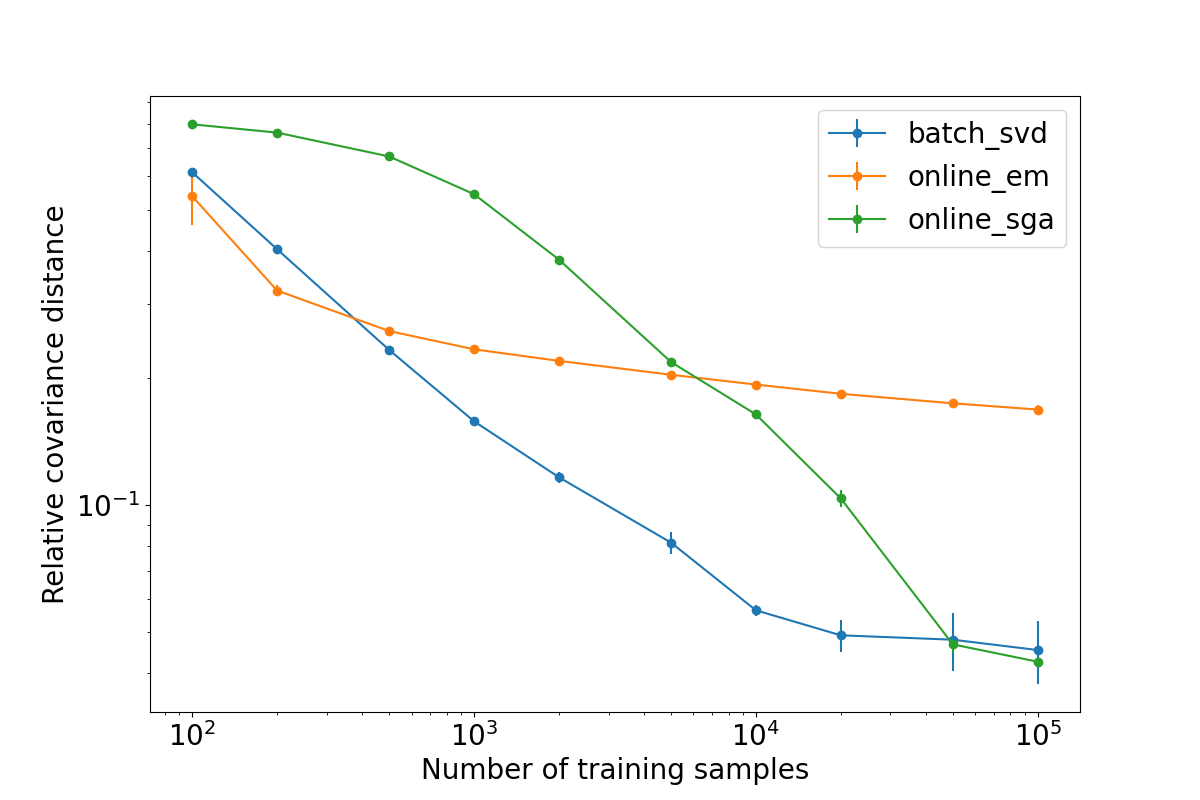
\includegraphics[width=70mm]{plots/online_fa_covar_distance__observation_dim=100__latent_dim=10__spectrum_min=1__spectrum_max=10.png}
		 & 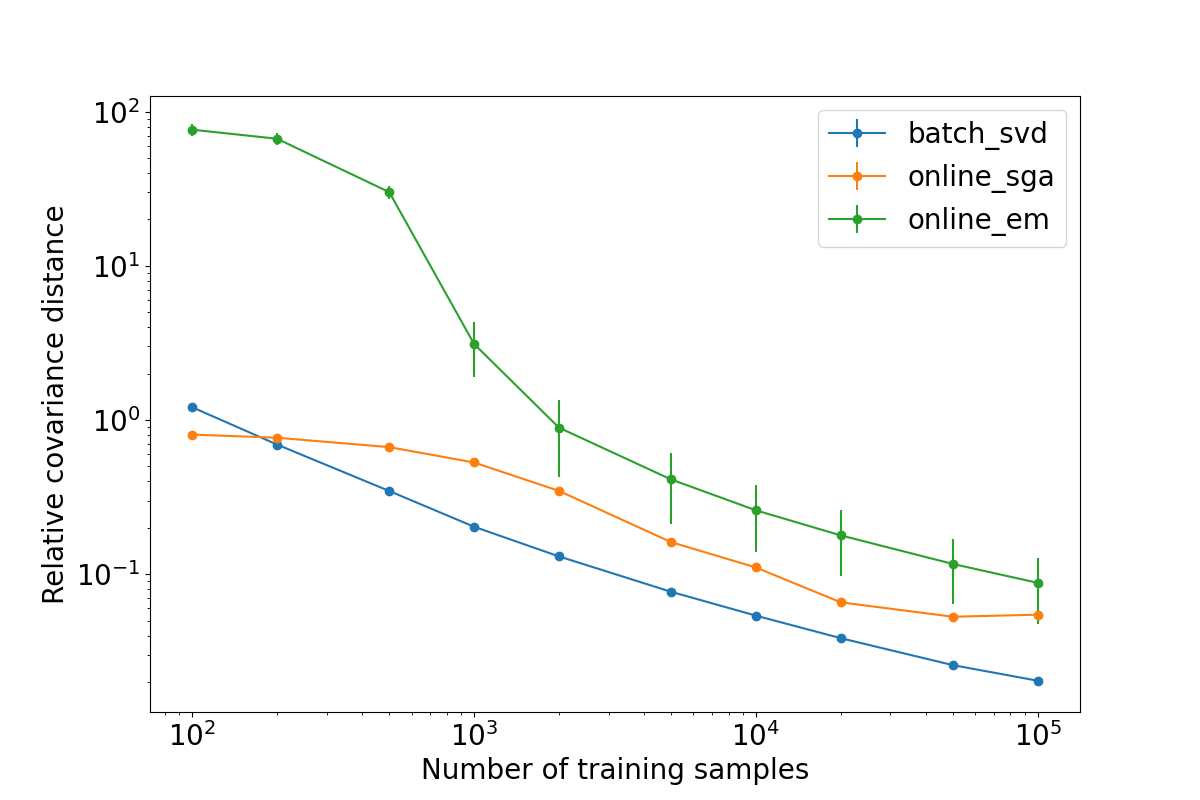
\includegraphics[width=70mm]{plots/online_fa_covar_distance__observation_dim=1000__latent_dim=10__spectrum_min=1__spectrum_max=10.png} \\
		 (a) $D=100$, $K=10$, $\matr{s}^2 \sim \mathcal{U}(1, 10)$ 
		 & (b) $D=1000$, $K=10$, $\matr{s}^2 \sim \mathcal{U}(1, 10)$\\[6pt]
		 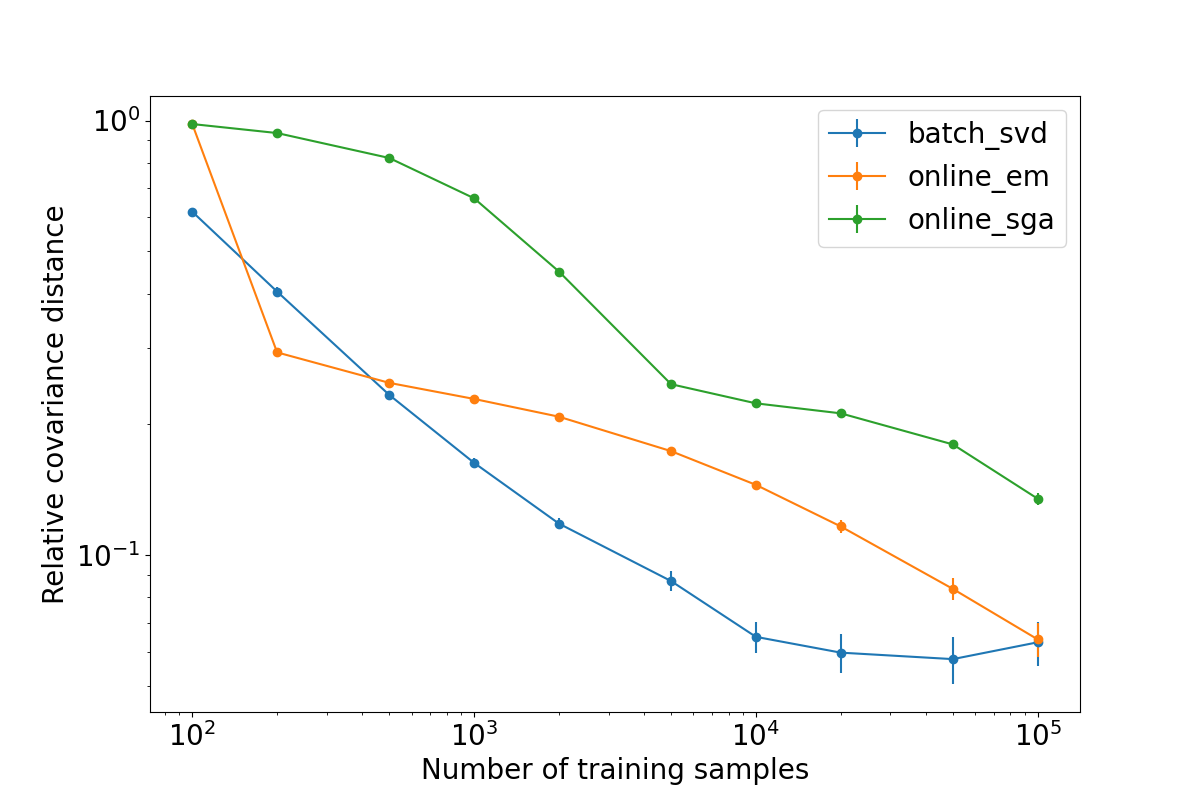
\includegraphics[width=70mm]{plots/online_fa_covar_distance__observation_dim=100__latent_dim=10__spectrum_min=1__spectrum_max=100.png}
		 & 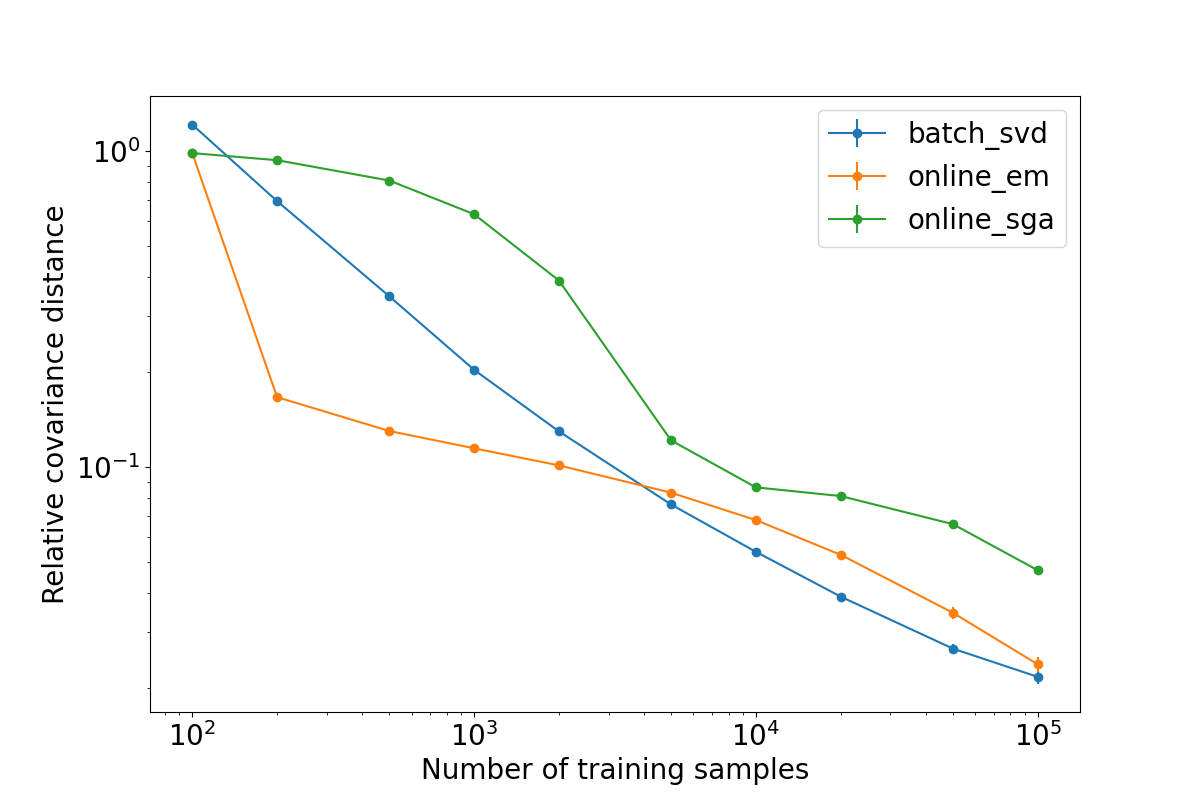
\includegraphics[width=70mm]{plots/online_fa_covar_distance__observation_dim=1000__latent_dim=10__spectrum_min=1__spectrum_max=100.png} \\
		 (c) $D=100$, $K=10$, $\matr{s}^2 \sim \mathcal{U}(1, 100)$ 
		 & (d) $D=1000$, $K=10$, $\matr{s}^2 \sim \mathcal{U}(1, 100)$\\[6pt]
		 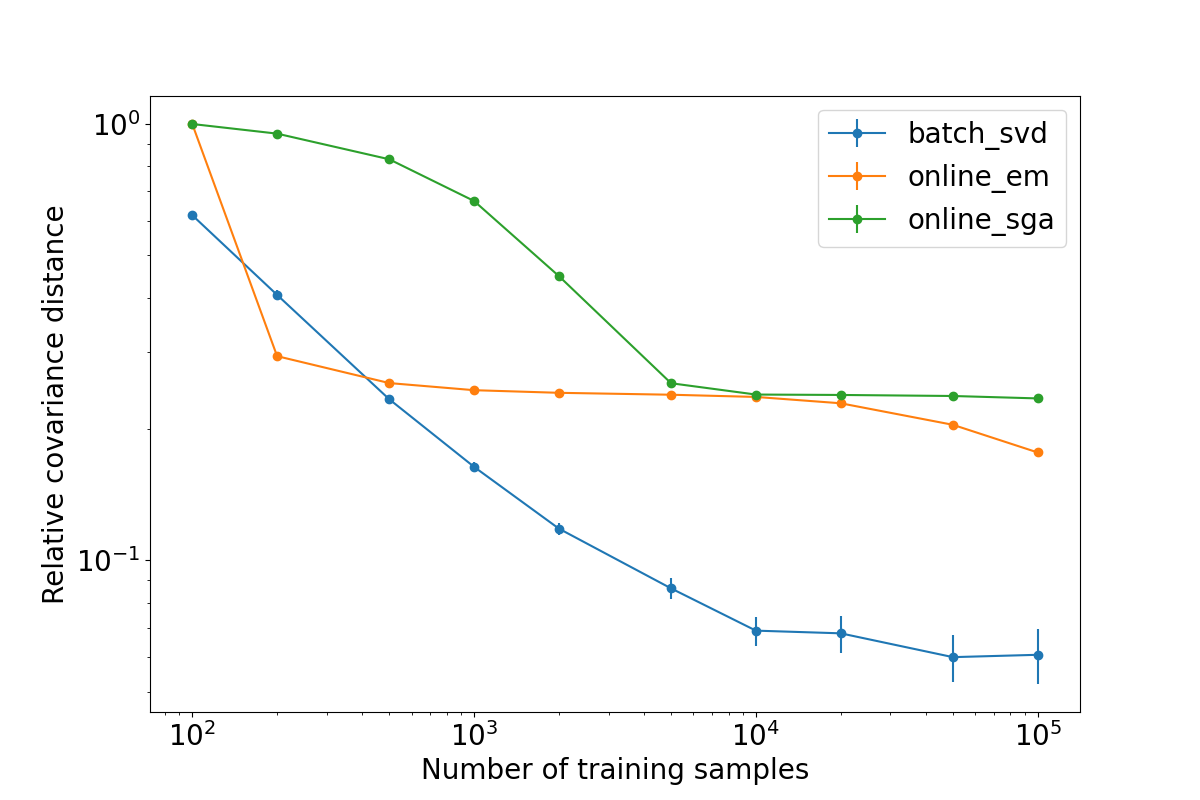
\includegraphics[width=70mm]{plots/online_fa_covar_distance__observation_dim=100__latent_dim=10__spectrum_min=1__spectrum_max=1000.png}
		 & 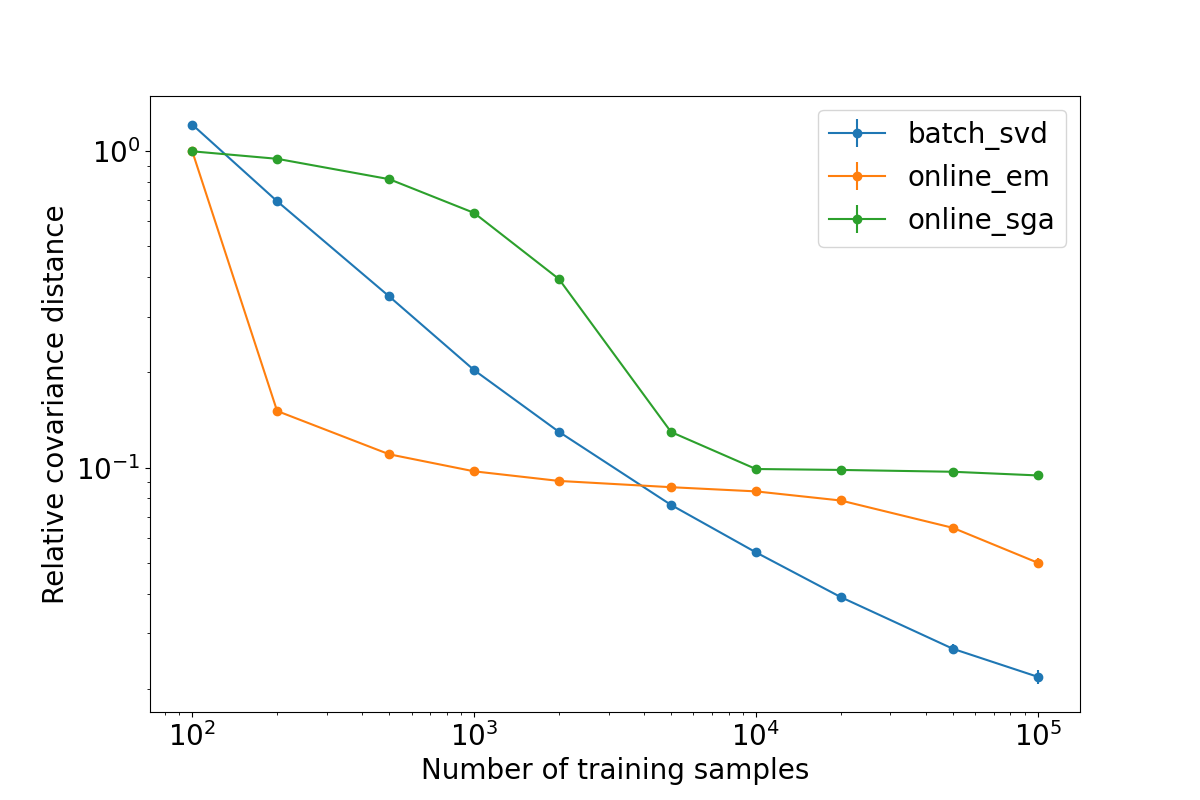
\includegraphics[width=70mm]{plots/online_fa_covar_distance__observation_dim=1000__latent_dim=10__spectrum_min=1__spectrum_max=1000.png} \\
		 (e) $D=100$, $K=10$, $\matr{s}^2 \sim \mathcal{U}(1, 1000)$ 
		 & (f) $D=1000$, $K=10$, $\matr{s}^2 \sim \mathcal{U}(1, 1000)$\\[6pt]
	\end{tabular}
	\caption{The relative distance of the estimated FA covariance matrices from the true covariance matrix as a function of the number of samples used to learn the models. The blue, orange and green lines show, for batch SVD, online EM and online SGA, respectively, the Frobenius norm of the difference between the true covariance matrix and the estimated covariance matrix divided by the Frobenius norm of the true covariance matrix. Each data point shows the mean value over ten trials with different random seeds, and standard error bars are also plotted. The different plots correspond to different combinations of the observation dimension $D$, the latent dimension $K$ and the range of the spectrum $\matr{s}^2$.} 
	\label{fig:fa_covar_distance}
\end{figure}

\subsection{Posterior Estimation with Synthetic Data}\label{sec:online_fa_posterior_experiments}

The ability of online EM to learn the posterior of a neural network's parameter vector hinges on obtaining samples of the parameter vector which are representative of the true posterior. In SWAG, such samples are thought to be obtained from the iterates of the parameter vector which are encountered along the SGD trajectory while training the neural network with a high constant learning rate, following an initial pre-training phase \cite{maddox2019}. In the case of linear regression - which is a neural network with no hidden layers - this assumption can be tested directly, since the true posterior of its parameter vector can be computed in closed form. Recall, however, that the linear regression posterior distribution in Equation (\ref{eqn:linear_regression_posterior}) refers to specific values of $\alpha$ and $\beta$. More specifically, in Equation (\ref{eqn:linear_regression_log_posterior}), the log-posterior of $\theta$ is written as 
\begin{equation}
	\log p(\theta | \mathcal{D}) 
	= -\frac{\beta}{2} \sum_{n=1}^N \big(y_n - \theta^\intercal \matr{x}_n \big)^2 
	-\frac{\alpha}{2} \theta^\intercal \theta 
	+ \text{constant}.
\end{equation}
Hence, the maximum \emph{a posteriori} (MAP) estimate of $\theta$ is that which maximises
\begin{equation}
	-\frac{\beta}{2} \sum_{n=1}^N \big(y_n - \theta^\intercal \matr{x}_n \big)^2 
	-\frac{\alpha}{2} \theta^\intercal \theta.
\end{equation}
Since $\beta > 0$, it is equivalent to minimise this expression scaled by $-\frac{2}{\beta}$. That is,
\begin{equation}
	\sum_{n=1}^N \big(y_n - \theta^\intercal \matr{x}_n \big)^2 
	+ \lambda \theta^\intercal \theta,
\end{equation}
where $\lambda = \frac{\alpha}{\beta}$. Note that this objective is exactly the same as the L2-regularised training loss used in non-Bayesian linear regression \cite{barber2007}. This means that, given data $\mathcal{D}$ and particular values of $\alpha$ and $\beta$, the SGD iterates sampled while training a linear regression model with data $\mathcal{D}$ and regularisation strength $\lambda = \frac{\alpha}{\beta}$ should in theory by representative of the true posterior $p(\theta | \mathcal{D})$.

In order to test this hypothesis, synthetic data was generated as follows. First, 1000 inputs $\matr{x} \in \R^2$ were sampled from a multivariate zero mean Gaussian distribution with unit variances and covariances of 0.5. Next, the parameter vector $\theta \in \R^2$ was sampled from $\mathcal{N}\big(\matr{0}, \alpha^{-1} \matr{I} \big)$ with $\alpha = 0.01$. Then the outputs $y \in \R$ were generated according to Equation (\ref{eqn:linear_regression}) with $\beta = 0.1$. Using this data, the true posterior was evaluated according to Equation (\ref{eqn:linear_regression_posterior}). For the purpose of obtaining samples from the posterior, an unregularised linear regression model was pre-trained for 500 epochs of SGD with a learning rate of 0.001 and a batch size of 100. Then, starting from the pre-trained model, a further 100 epochs of SGD were executed with the same batch size but with a learning rate of $0.1$ and the regularisation parameter set to $\lambda = \frac{\alpha}{\beta} = 0.1$. During these final 100 epochs, the parameter vector sampled after each mini-batch gradient update was used to iteratively fit an approximate FA posterior with latent dimension $K=1$ via online EM (Algorithm \ref{alg:online_em}).


\subsubsection{Results and Discussion}

Figure \ref{fig:true_posterior_vs_online_em} shows a qualitative comparison between the true and approximate posteriors. The posterior learned by online EM is extremely poor. As well as the covariance being too small and in the wrong direction, the approximate posterior mean is significantly different from the true value. Since online EM computes the mean of the SGD iterates exactly, this suggests that the sampled iterates are not representative of the true posterior. 
\begin{figure}[!htbp] 
	\begin{tabular}{cc}
		 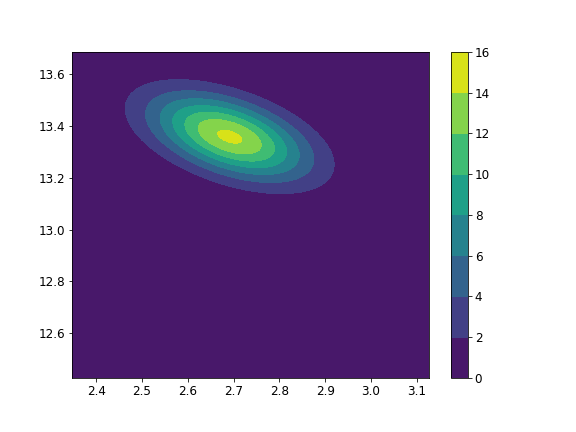
\includegraphics[width=70mm]{plots/linear_model_poor_estimation_true_posterior__alpha=0.01__beta=0.1.png}
		 & 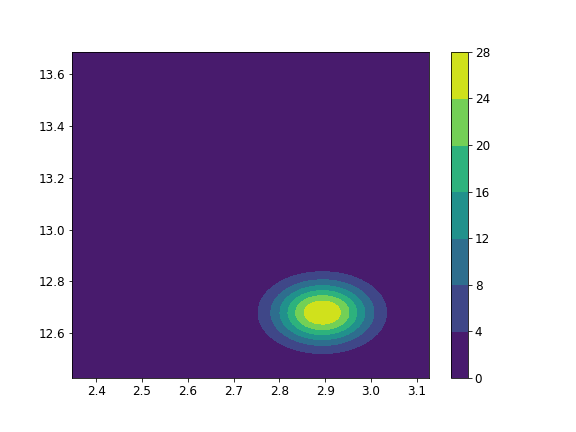
\includegraphics[width=70mm]{plots/linear_model_poor_estimation_online_em__alpha=0.01__beta=0.1__latent_dim=1.png} \\
		 (a) Ground truth
		 & (b) Online EM FA \\[6pt]
	\end{tabular}
	\caption{The true posterior pdf of a linear regression model with two learnable parameters, plus the pdf of a FA model with a single latent dimension which was fit to the SGD iterates via online EM.}
	\label{fig:true_posterior_vs_online_em}
\end{figure}

Further analysis revealed that this is indeed the case. Figure \ref{fig:linear_regression_pdfs} shows the SGD iterates plotted on top of the true posterior for different combinations of the learning rate and the regularisation strength. Note that in each case the pre-trained parameter vector is close to the true posterior mean. However, when $\lambda = 0.1$ (subplots (a) and (c)), SGD then moves away from the pre-trained solution to a different region of the parameter space. When $\lambda = 0.001$ (subplots (b) and (d)), SGD does bounce around the true posterior mean, but the empirical covariance is in the wrong direction and far too narrow when the learning rate is $0.01$.
\begin{figure}[!htbp] 
	\begin{tabular}{cc}
		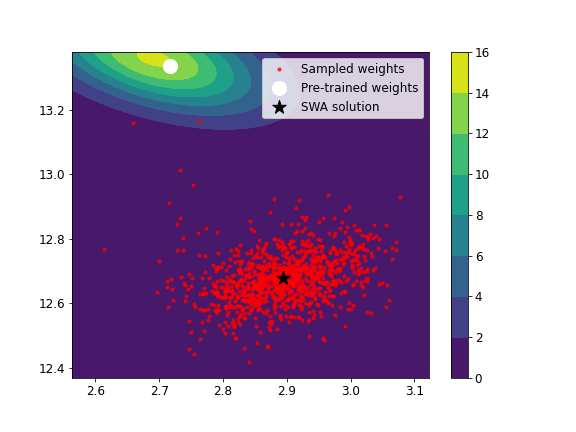
\includegraphics[width=70mm]{plots/linear_model_weight_iterates__lr=0.1__lambda=0.1.png}
		& 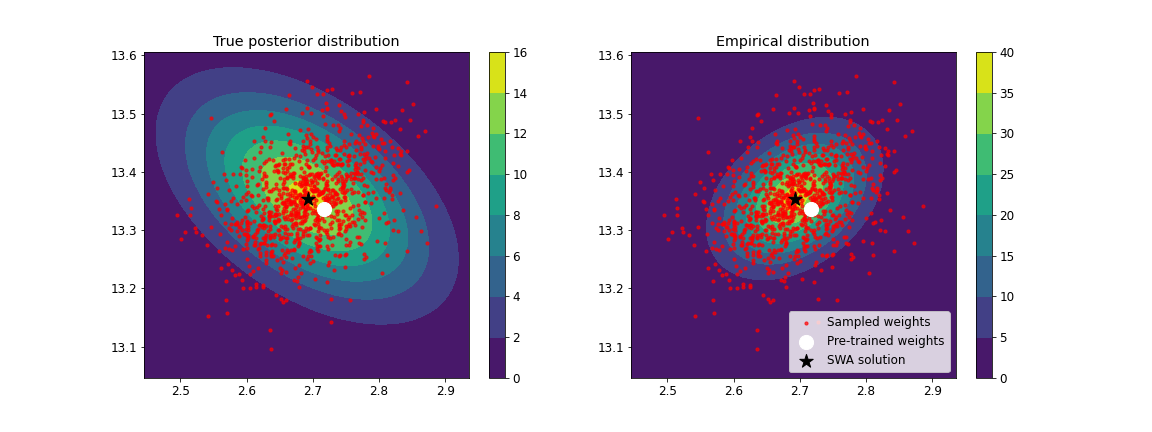
\includegraphics[width=70mm]{plots/linear_model_weight_iterates__lr=0.1__lambda=0.001.png} \\
		(a) Learning rate of 0.1 and $\lambda = 0.1$
		 & (b) Learning rate of 0.1 and $\lambda = 0.001$ \\[6pt] 
		 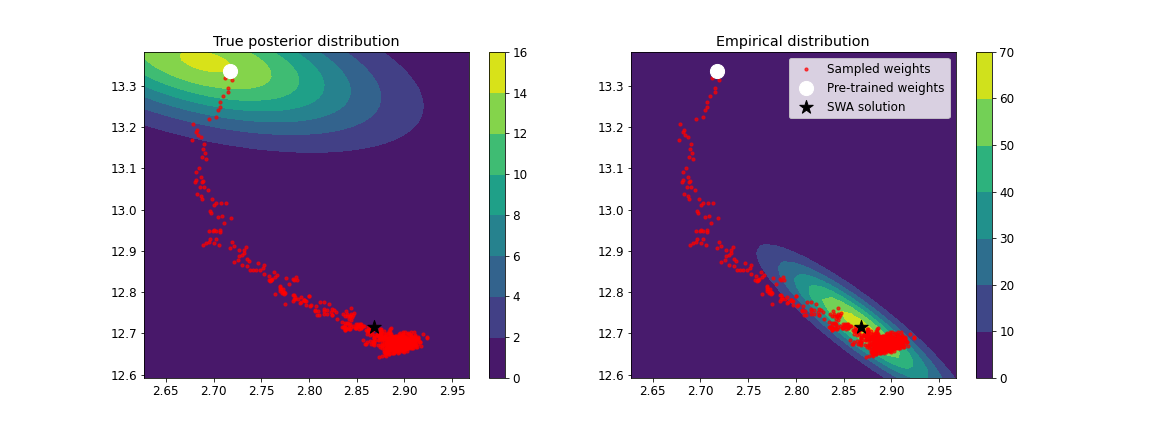
\includegraphics[width=70mm]{plots/linear_model_weight_iterates__lr=0.01__lambda=0.1.png}
		 & 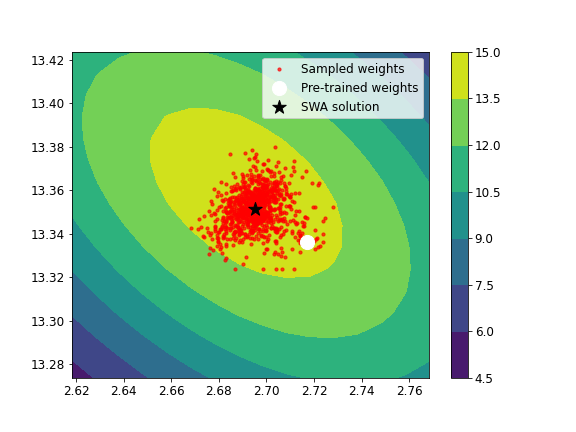
\includegraphics[width=70mm]{plots/linear_model_weight_iterates__lr=0.01__lambda=0.001.png} \\
		 (c) Learning rate of 0.01 and $\lambda = 0.1$
		 & (d) Learning rate of 0.01 and $\lambda = 0.001$ \\[6pt]
	\end{tabular}
	\caption{Parameter vectors sampled while training a linear regression model via SGD, for different combinations of learning rate and regularisation strength. 
	}
	\label{fig:linear_regression_pdfs}
\end{figure}

The most that can be expected of online EM is that it fits the SGD iterates well. If the iterates are not representative of the true posterior, applying online EM will not result in good posterior estimation. In these experiments it was not even possible to obtain representative samples of a very simple linear regression posterior with only two dimensions. Perhaps for some combination of the batch size, learning rate and regularisation strength this is possible. However, in the case of a non-linear neural network the true posterior is not known, making hyperparameter optimisation extremely difficult. Therefore, methods based on SWAG are unlikely to achieve good posterior covariance estimation in practice. Fortunately, there are more direct approaches which do not rely on a separate posterior sampling procedure. One such algorithm is described next in Chapter \ref{ch:vifa}.


\chapter{Variational Inference with a Factor Analysis Posterior}\label{ch:vifa}

This chapter presents VIFA, a VI-based approach to learning a FA posterior of a neural network. Unlike Algorithms \ref{alg:gradient_fa} and \ref{alg:online_em}, VIFA does not require that samples from the posterior are obtained via some separate procedure. 

\section{VIFA}

In Section \ref{sec:vi}, a general VI algorithm was outlined for learning an approximate Gaussian posterior of the parameter vector of a neural network. Suppose that the approximate posterior is a FA model. That is, $q(\theta) = \mathcal{N}\big(\matr{c}, \matr{FF}^{\intercal} + \Psi\big)$ for some $\matr{c} \in \R^D$, $\matr{F} \in \R^{D \times K}$ and $D \times D$ diagonal matrix $\Psi$. Then the gradient of the VI objective in Equation (\ref{eqn:vi_objective}) becomes 
\begin{equation}\label{eqn:vi_fa_derivatives}
	\nabla_{\matr{c}, \matr{F}, \Psi} \E_{q(\theta)} [\log q(\theta)]
	- \nabla_{\matr{c}, \matr{F}, \Psi} \E_{q(\theta)} [\log p(\theta)]
	-  \nabla_{\matr{c}, \matr{F}, \Psi} \E_{q(\theta)} [\log p(\mathcal{D} | \theta)],
\end{equation}
where the expectation is taken over samples $\theta \sim \mathcal{N}\big(\matr{c}, \matr{FF}^{\intercal} + \Psi\big)$. These derivatives are derived in the following sections. 


\subsection{Partial Derivatives of the Variational Distribution}

The logarithm of the pdf of the variational distribution is
\begin{equation}
	\log q(\theta)
	= -\frac{1}{2} (\theta - \matr{c})^\intercal (\matr{FF}^{\intercal} + \Psi)^{-1} (\theta - \matr{c})  
	- \frac{1}{2} \log |\matr{FF}^{\intercal} + \Psi| 
	- \frac{D}{2} \log 2\pi.
\end{equation}
It is given in \cite{petersen2012} that, for any symmetric matrix $\matr{A}$ and stochastic vector $\matr{x}$ with mean $\matr{m}$ and covariance $\matr{M}$,
\begin{equation}\label{eqn:expectation_xTAx}
	\E [\matr{x}^\intercal \matr{A} \matr{x}] = \tr(\matr{A}\matr{M}) + \matr{m}^\intercal \matr{A} \matr{m}.
\end{equation}
Setting $\matr{S} = \matr{FF}^{\intercal} + \Psi$ and noting that $\theta - \matr{c}$ has mean $\matr{0}$ and covariance $\matr{S}$ over $q(\theta)$, it follows that
\begin{align}
\begin{split}\label{eqn:expectation_of_vi_dist}
	\E_{q(\theta)}[\log q(\theta)]
	& = -\frac{1}{2} \tr\big(\matr{S}^{-1} \matr{S} \big) -\frac{1}{2} \matr{0} \matr{S}^{-1} \matr{0} 
	- \frac{1}{2} \log |\matr{S}| - \frac{D}{2} \log 2\pi \\
	& = -\frac{1}{2}\tr(\matr{I}) - \frac{1}{2} \log |\matr{S}| - \frac{D}{2} \log 2\pi \\
	& = -\frac{D}{2}  - \frac{1}{2} \log |\matr{S}| - \frac{D}{2} \log 2\pi.
\end{split}
\end{align}
Hence, 
\begin{equation}
	\nabla_\matr{c} \E_{q(\theta)} [\log q(\theta)] = \matr{0}
\end{equation}
and, using the identity $\nabla_\matr{X} \log |\matr{X}| = \matr{X}^{-\intercal}$ from \cite{petersen2012} and the fact that $\matr{S}$ is symmetric,
\begin{equation}
	\nabla_\matr{S} \E_{q(\theta)} [\log q(\theta)] = -\frac{1}{2} \matr{S}^{-1}.
\end{equation}
It then follows from the chain rule of calculus that
\begin{align}
\begin{split}\label{eqn:grad_vi_dist_wrt_F}
	\nabla_\matr{F} \E_{q(\theta)} [\log q(\theta)]
	%& = -\frac{1}{2} \matr{S}^{-1} (\nabla_\matr{F} \matr{S}) \\
	& = -\frac{1}{2} \matr{S}^{-1} (2\matr{F}) \\
	& = -\matr{S}^{-1}\matr{F}
\end{split}
\end{align}
and
\begin{align}
\begin{split}\label{eqn:grad_vi_dist_wrt_Psi}
	\nabla_\Psi \E_{q(\theta)} [\log q(\theta)]
	%& = \diag\Big(\diag\Big(-\frac{1}{2} \matr{S}^{-1} (\nabla_\Psi \matr{S}) \Big)\Big) \\
	& = -\frac{1}{2} \diag\big(\diag\big(\matr{S}^{-1} \matr{I}\big)\big) \\
	& = -\frac{1}{2} \diag\big(\diag\big(\matr{S}^{-1}\big)\big).
\end{split}
\end{align}

\subsection{Partial Derivatives of the Prior}

Let the prior be $p(\theta) = \mathcal{N}(\matr{0}, \alpha^{-1} \matr{I})$ for some precision $\alpha > 0$. Then
\begin{align}
\begin{split}
	\E_{q(\theta)} [\log p(\theta)]
	& = \E_{q(\theta)} \Big[-\frac{1}{2} \theta^\intercal \alpha \matr{I} \theta  - \frac{1}{2} \log |\alpha^{-1} \matr{I}| - \frac{D}{2} \log 2\pi\Big] \\
	& = -\frac{\alpha}{2} \E_{q(\theta)} \Big[ \theta^\intercal \matr{I} \theta \Big] + \text{constant} \\
	& = -\frac{\alpha}{2}\big( \tr(\matr{FF}^{\intercal} + \Psi) + \matr{c}^\intercal \matr{c} \big)+ \text{constant},
\end{split}
\end{align}
where the last line follows from Equation (\ref{eqn:expectation_xTAx}). Hence, 
\begin{equation}
	\nabla_\matr{c} \E_{q(\theta)} [\log p(\theta)] = -\alpha \matr{c},
\end{equation}
\begin{equation}
	\nabla_\matr{F} \E_{q(\theta)} [\log p(\theta)] = -\alpha \matr{F},
\end{equation}
\begin{equation}\label{eqn:grad_prior_wrt_psi}
	\nabla_\Psi \E_{q(\theta)} [\log p(\theta)] = -\frac{\alpha}{2} \matr{I},
\end{equation}
which follow from the matrix calculus identities in \cite{petersen2012}.

\subsection{Partial Derivatives of the Likelihood}

Let the log-likelihood, $\log p(\mathcal{D} | \theta)$, be parameterised by a neural network with weights $\theta$. Due to the functional form of a non-linear neural network, $\E_{q(\theta)} [\log p(\mathcal{D} | \theta)]$ cannot be computed in closed-form. Recall from Section \ref{sec:vi} that a Monte Carlo estimate can instead be constructed from mini-batches of training data. Formally, 
\begin{equation}
	 \E_{q(\theta)} [\log p(\mathcal{D} | \theta)]
	\approx \frac{1}{L} \sum_{l=1}^{L} \Bigg( \frac{N}{M} \sum_{(\matr{x}, y) \in \mathcal{B}_l} \log p(y | \matr{x}, \theta_l) \Bigg),
\end{equation}
where $L$ is the Monte Carlo average size, each $\mathcal{B}_l$ is a mini-batch of $M$ training examples sampled from the full dataset $\mathcal{D}$ of size $N$ and $\theta_l \sim q(\theta)$. In order to obtain the partial derivatives of this expression with respect to $\matr{c}$, $\matr{F}$ and $\Psi$, the re-parameterisation trick \cite{goodfellow2016} can be used. First note that, by re-writing Equation (\ref{eqn:fa_model}), sampling $\theta_l \sim q(\theta) = \mathcal{N}\big(\matr{c}, \matr{FF}^{\intercal} + \Psi\big)$ is equivalent to setting  
\begin{equation}\label{eqn:fa_reparam_trick}
	\theta_l = \matr{F}\matr{h}_l + \matr{c} + \Psi^{1/2} \matr{z}_l
\end{equation}
from some $\matr{h}_l \sim p(\matr{h}) = \mathcal{N}(\matr{0}^K, \matr{I}^{K \times K})$ and $\matr{z}_l \sim p(\matr{z}) = \mathcal{N}(\matr{0}^D, \matr{I}^{D \times D})$, where the exponent is applied to $\Psi$ element-wise. 
%Then
%\begin{align}
%\begin{split}
%	\E_{q(\theta)} [\log p(\mathcal{D} | \theta)]
%	& = \E_{p(\matr{h})p(\matr{z})} [\log p(\mathcal{D} | \theta)] \\
%	& \approx \frac{1}{L} \sum_{l=1}^{L} \Bigg( \frac{N}{M} \sum_{(\matr{x}, y) \in \mathcal{B}_l} \log p(y | \matr{x}, \theta_l) \Bigg),
%\end{split}
%\end{align}
%where each $\theta_l$ is sampled according to Equation (\ref{eqn:fa_reparam_trick}). 
It then follows that
\begin{align}
\begin{split}\label{eqn:expected_grad_log_likelihood}
	\nabla_{\matr{c}, \matr{F}, \Psi} \E_{q(\theta)} [\log p(\mathcal{D} | \theta)]
	& = \nabla_{\matr{c}, \matr{F}, \Psi} \E_{p(\matr{h})p(\matr{z})} [\log p(\mathcal{D} | \theta)] \\
	& \approx -\frac{1}{L} \sum_{l=1}^{L} \Bigg(N \cdot \nabla_{\matr{c}, \matr{F}, \Psi} \Bigg( -\frac{1}{M} \sum_{(\matr{x}, y) \in \mathcal{B}_l} \log p(y | \matr{x}, \theta_l) \Bigg) \Bigg).
\end{split}
\end{align}
Since $\theta_l = \matr{F}\matr{h}_l + \matr{c} + \Psi^{1/2} \matr{z}_l$, the chain rule of calculus can be used to obtain these partial derivatives. Formally,
\begin{equation}
	 \nabla_\matr{c} \E_{q(\theta)} [\log p(\mathcal{D} | \theta)]
	 \approx -\frac{1}{L} \sum_{l=1}^{L} N \matr{g}_{\theta_l},
\end{equation}
\begin{equation}
	 \nabla_\matr{F} \E_{q(\theta)} [\log p(\mathcal{D} | \theta)]
	 \approx -\frac{1}{L} \sum_{l=1}^{L} N \matr{g}_{\theta_l} \matr{h}_l^\intercal,
\end{equation}
\begin{equation}\label{eqn:grad_likelihood_wrt_psi}
	 \nabla_\Psi \E_{q(\theta)} [\log p(\mathcal{D} | \theta)]
	 \approx \diag\Bigg( \diag\Bigg( -\frac{1}{L} \sum_{l=1}^{L} \frac{N}{2} \matr{g}_{\theta_l} \matr{z}_l^\intercal \Psi^{-1/2} \Bigg)\Bigg),
\end{equation}
where
\begin{equation}
	\matr{g}_{\theta_l} = \nabla_{\theta_l} \Bigg( -\frac{1}{M} \sum_{(\matr{x}, y) \in \mathcal{B}_l} \log p(y | \matr{x}, \theta_l) \Bigg).
\end{equation}
Note that $\matr{g}_{\theta_l}$ is the gradient of the average negative log-likelihood of $\theta_l$, where the average is computed over the training examples in the mini-batch $\mathcal{B}_l$. This is convenient, since this quantity can be computed efficiently using the back-propagation algorithm \cite{rumelhart1986}. Indeed, deep learning frameworks such as PyTorch \cite{paszke2019} compute $\matr{g}_{\theta_l}$ as standard. 


\subsection{Practical Implementation}

In order to compute the partial derivatives in Equations (\ref{eqn:grad_vi_dist_wrt_F}) and (\ref{eqn:grad_vi_dist_wrt_Psi}), the inverse of $\matr{S} = \matr{FF}^{\intercal} + \Psi$ is required. Using the Woodbury identity \cite{petersen2012},
\begin{align}
\begin{split}
	( \matr{FF}^{\intercal} + \Psi)^{-1}
	& = \Psi^{-1} - \Psi^{-1}\matr{F}(\matr{I} + \matr{F}^\intercal \Psi^{-1} \matr{F})^{-1} \matr{F}^\intercal \Psi^{-1} \\
	& = \Psi^{-1} - (\psi^{-1} \odot \matr{F}) \big(\matr{I} + \matr{F}^\intercal (\psi^{-1} \odot \matr{F})\big)^{-1} (\psi^{-1} \odot \matr{F})^\intercal \\
	& = \Psi^{-1} - \matr{A} (\matr{I} + \matr{F}^\intercal \matr{A})^{-1} \matr{A}^\intercal,
\end{split}
\end{align}
where $\psi = \diag(\Psi)$ and $\matr{A} = \psi^{-1} \odot \matr{F}$ (with broadcasting). It follows that
\begin{align}
\begin{split}
	\nabla_\matr{F} \E_{q(\theta)} [\log q(\theta)]
	& = -( \matr{FF}^{\intercal} + \Psi)^{-1}\matr{F} \\
	& = -\Psi^{-1} \matr{F}  + \matr{A}  (\matr{I} + \matr{F}^\intercal \matr{A})^{-1} (\matr{A}^\intercal \matr{F}) \\
	& = -\matr{A}  + \matr{A} (\matr{I} + \matr{F}^\intercal \matr{A})^{-1} (\matr{A}^\intercal \matr{F}) \\
	& = -\matr{A}  + \matr{A} (\matr{I} + \matr{B})^{-1} \matr{B}^\intercal \\
	& = -\matr{A}  + \matr{C} \matr{B}^\intercal,
\end{split}
\end{align}
where $\matr{B} = \matr{F}^\intercal \matr{A}$ and $\matr{C} = \matr{A} (\matr{I} + \matr{B})^{-1}$. Also,
\begin{align}
\begin{split}
	\nabla_\psi \E_{q(\theta)} [\log q(\theta)]
	& = -\frac{1}{2} \diag\big( ( \matr{FF}^{\intercal} + \Psi)^{-1}\big) \\
	& = -\frac{1}{2}\diag\big(\Psi^{-1}  - \matr{A}  (\matr{I} + \matr{F}^\intercal \matr{A})^{-1} \matr{A}^\intercal \big) \\
	& = -\frac{1}{2}\psi^{-1} + \frac{1}{2} \diag\big(\matr{C} \matr{A}^\intercal \big) \\
	& = -\frac{1}{2}\psi^{-1} + \frac{1}{2} \text{sum}\big(\matr{C} \odot \matr{A}, \text{ dim} = 1\big).
\end{split}
\end{align}
Note that these partial derivatives involve no explicit use of $D \times D$ matrices. All other references to $D \times D$ matrices can be removed by writing the partial derivatives in Equations (\ref{eqn:grad_prior_wrt_psi}) and (\ref{eqn:grad_likelihood_wrt_psi}) with respect to $\psi$ rather than $\Psi$. Formally,
\begin{equation}
	\nabla_\psi \E_{q(\theta)} [\log p(\theta)] = -\frac{\alpha}{2} \matr{1}^D,
\end{equation}
\begin{equation}
	\nabla_\psi \E_{q(\theta)} [\log p(\mathcal{D} | \theta)]
	 \approx  -\frac{1}{L} \sum_{l=1}^{L} \frac{N}{2} \matr{g}_{\theta_l} \odot \big(\psi^{-1/2} \odot \matr{z} \big).
\end{equation}
Finally, as in Algorithm \ref{alg:gradient_fa}, the re-parameterisation $\psi = \exp \gamma$ can again be used to ensure that the variances remain positive. Since $\nabla_\gamma \psi = \psi$, it follows from the chain rule that the corresponding partial derivatives with respect to $\gamma$ are 
\begin{equation}
	\nabla_\gamma \E_{q(\theta)} [\log q(\theta)] = -\frac{1}{2} + \frac{1}{2} \text{sum}\big(\matr{C} \odot \matr{A}, \text{ dim} = 1\big) \odot \psi,
\end{equation}
\begin{equation}
	\nabla_\gamma \E_{q(\theta)} [\log p(\theta)] = -\frac{\alpha}{2} \psi,
\end{equation}
\begin{equation}
	\nabla_\gamma \E_{q(\theta)} [\log p(\mathcal{D} | \theta)]
	 \approx  -\frac{1}{L} \sum_{l=1}^{L} \frac{N}{2} \matr{g}_{\theta_l} \odot \big(\psi^{1/2} \odot \matr{z} \big).
\end{equation}
Collecting the partial derivatives in Equation (\ref{eqn:vi_fa_derivatives}), the final update rules are
 \begin{equation}\label{eqn:vifa_c_update}
	\matr{c} \leftarrow \matr{c} - \eta_\matr{c}\Bigg(
	\alpha \matr{c} + \frac{1}{L} \sum_{l=1}^{L} N \matr{g}_{\theta_l}
	\Bigg),
\end{equation}
 \begin{equation}\label{eqn:vifa_F_update}
	\matr{F} \leftarrow \matr{F} - \eta_\matr{F}\Bigg(
	-\matr{A}  + \matr{C} \matr{B}^\intercal+ \alpha \matr{F} + \frac{1}{L} \sum_{l=1}^{L} N \matr{g}_{\theta_l} \matr{h}_l^\intercal
	\Bigg),
\end{equation}
\begin{equation}\label{eqn:vifa_gamma_update}
	\gamma \leftarrow \gamma - \eta_\gamma\Bigg(
	-\frac{1}{2} + \frac{1}{2} \text{sum}\big(\matr{C} \odot \matr{A}, \text{ dim} = 1\big) \odot \psi
	+\frac{\alpha}{2} \psi + \frac{1}{L} \sum_{l=1}^{L} \frac{N}{2} \matr{g}_{\theta_l} \odot \big(\psi^{1/2} \odot \matr{z} \big)
	\Bigg)
\end{equation}
for learning rates $\eta_\matr{c},  \eta_\matr{F}, \eta_\gamma > 0$. Pseudo code for the practical implementation is given in Algorithm \ref{alg:vi_fa}. Being a VI method for approximating a posterior with a FA model, the algorithm is named VIFA.

\begin{algorithm}[!htbp] 
	\caption{VIFA}
	\label{alg:vi_fa}
	\begin{algorithmic}[1]
		\Require{Dataset $\mathcal{D} = \{(\matr{x}_n, y_n)\}_{n=1}^N$, observation dimension $D$, latent dimension $K$, prior precision $\alpha > 0$, iterations $T$, mini-batch size $M$, Monte Carlo average size $L$, learning rates $\eta_\matr{c},  \eta_\matr{F}, \eta_\gamma > 0$} 
		\State Initialise $\matr{c} = \matr{0}^D$, $\matr{F} \in \R^{D \times K}$, $\psi = \matr{1}^D$
		\State $\gamma \leftarrow \log \psi$
		\State Initialise $\hat{\matr{g}}_\matr{c} = \matr{0}^D$, $\hat{\matr{G}}_\matr{F} = \matr{0}^{D \times K}$, $\hat{\matr{g}}_\gamma = \matr{0}^D$
		\State $\matr{A} \leftarrow \psi^{-1} \odot \matr{F}$ (with broadcasting)
		\State $\matr{B} \leftarrow \matr{F}^\intercal \matr{A}$
		\State $\matr{C} \leftarrow \matr{A} (\matr{I} + \matr{B})^{-1}$
		\For {$t = 1,\dots, T$}
			\State Sample a mini-batch $\mathcal{B}$ of $M$ training examples from $\mathcal{D}$
			\State Sample $\matr{h} \sim \mathcal{N}(\matr{0}^K, \matr{I}^{K \times K})$
			\State Sample $\matr{z} \sim \mathcal{N}(\matr{0}^D, \matr{I}^{D \times D})$
			\State $\theta \leftarrow \matr{Fh} + \matr{c} + \psi^{1/2} \odot \matr{z}$
			\State $\matr{g}_\theta \leftarrow \nabla_\theta \big(-\frac{1}{M} \sum_{(\matr{x}, y) \in \mathcal{B}} \log p(y | \matr{x}, \theta)\big)$ 
			(via back-propagation)
			\State $\hat{\matr{g}}_\matr{c} \leftarrow \hat{\matr{g}}_\matr{c} + N \hat{\matr{g}}_\theta$
			\State $\hat{\matr{G}}_\matr{F} \leftarrow \hat{\matr{G}}_\matr{F} + N \hat{\matr{g}}_\theta \matr{h}^\intercal$
			\State $\hat{\matr{g}}_\gamma \leftarrow \hat{\matr{g}}_\gamma + \frac{N}{2} \hat{\matr{g}}_\theta \odot \big(\psi^{1/2} \odot \matr{z}\big)$
			\If {$t \bmod L = 0$}
				\State $\matr{c} \leftarrow \matr{c} - \eta_\matr{c} \big(\alpha \matr{c} + \frac{1}{L}\hat{\matr{g}}_\matr{c}\big)$
				\State $\matr{F} \leftarrow \matr{F} - \eta_\matr{F} \big(-\matr{A}  + \matr{C} \matr{B}^\intercal+ \alpha \matr{F} +\frac{1}{L}\hat{\matr{G}}_\matr{F}\big)$
				\State $\gamma \leftarrow \gamma - \eta_\gamma \big(-\frac{1}{2} + \frac{1}{2} \text{sum}(\matr{C} \odot \matr{A}, \text{ dim} = 1) \odot \psi +\frac{\alpha}{2} \psi  + \frac{1}{L}\hat{\matr{g}}_\gamma\big)$
				\State $\psi \leftarrow \exp \gamma$
				\State Reset $\hat{\matr{g}}_\matr{c}, \hat{\matr{G}}_\matr{F}$ and $\hat{\matr{g}}_\gamma$ according to line 3
				\State Recalculate $\matr{A}, \matr{B}$ and $\matr{C}$ according to lines 4-6
			\EndIf
		\EndFor
	\State \Return $\matr{c}, \matr{F}, \psi$
	\end{algorithmic}
\end{algorithm}


\section{Experiments}

\subsection{Posterior Estimation with Synthetic Data}\label{sec:vifa_posterior_synthetic}

Synthetic data was generated in the exact same way as for the experiments in Section \ref{sec:online_fa_posterior_experiments}, for the same values of the prior precision $\alpha$ and the noise precision $\beta$. Using this data, the true posterior was evaluated according to Equation (\ref{eqn:linear_regression_posterior}) and an approximate posterior with latent dimension $K=1$ was estimated via VIFA. VIFA ran for 5000 epochs with a batch size of $M=100$ and a Monte Carlo average size of $L=10$.  The learning rates $\eta_\matr{c}$,  $\eta_\matr{F}$ and $\eta_\gamma$ were set to 0.01, 0.0001 and 0.01, respectively. The reason for using a smaller learning rate for $\matr{F}$ is that its contribution to the full covariance matrix is $\matr{F}\matr{F}^\intercal$. Since this is regression, the average negative log-likelihood term used on line 12 of Algorithm \ref{alg:vi_fa} was set to
\begin{equation}\label{eqn:vifa_log_likelihood_term}
	-\frac{1}{M} \sum_{(\matr{x}, y) \in \mathcal{B}} \log \mathcal{N}\big(y; f(\matr{x}; \theta), \beta^{-1}\big),
\end{equation}
where $f(\matr{x}; \theta)$ is the prediction of the linear regression model for input $\matr{x}$ and parameters $\theta$. Finally, to improve numerical stability, any gradients with Frobenius norm greater than 10 were rescaled to have norm of exactly 10. All experiments were repeated ten times. In each trial a different random seed was used for generating the data, the true parameter vector and the initial parameters of the linear regression model. 

\subsubsection{Results and Discussion}

The aggregated results of applying VIFA to the data are shown in Table \ref{table:linear_regression_vi_posterior}. A qualitative comparison between the true and approximate posteriors in also given in Figure \ref{fig:linear_regression_vi_posterior} for one of the ten trials. It can be seen that the contours of the approximate posterior are very similar to the ground truth in term of position, direction and density. In comparison to the equivalent results for the SWAG-based approach in Figure \ref{fig:true_posterior_vs_online_em}, VIFA does a much better job of approximating the true posterior covariance.

\begin{table}[h!]
	\begin{center}
		\begin{tabular}{|| p{0.3\linewidth} p{0.3\linewidth} p{0.3\linewidth} ||} 
 			\hline
 			Relative Distance from Mean & Relative Distance from Covariance & Scaled 2-Wasserstein Distance \\ [0.5ex] 
 			\hline\hline
			$0.0031 \pm 0.0005$ 	& $0.0983 \pm 0.0129$ 	& $0.0194 \pm 0.0023$ \\ [1ex] 
			\hline
		\end{tabular}
		\caption{Distances between the true posterior distribution of the parameter vector of a linear regression model and the approximate FA posterior estimated using VIFA. Relative distances between the true and approximate means and covariances are shown. Each relative distance is the Frobenius norm of the difference between the true parameter and the approximate parameter divided by the Frobenius norm of the true parameter. Also shown is the 2-Wasserstein distance between the true posterior Gaussian distribution and the approximate Gaussian distribution, divided by the dimension of the distribution. Each distance is the mean value over ten trials with different random seeds, and standard errors are also given.}
		\label{table:linear_regression_vi_posterior}
	\end{center}
\end{table}

\begin{figure}[!htbp] 
	\begin{tabular}{cc}
		 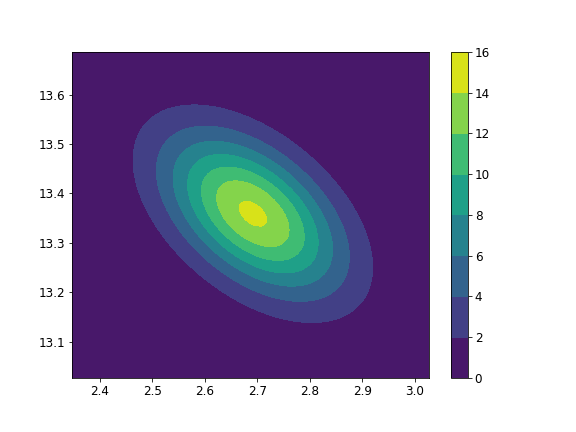
\includegraphics[width=70mm]{plots/linear_model_true_posterior__alpha=0.01__beta=0.1.png}
		 & 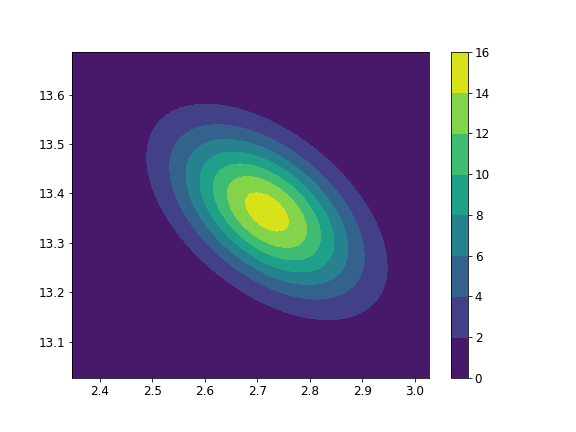
\includegraphics[width=70mm]{plots/linear_model_vi_posterior__alpha=0.01__beta=0.1__latent_dim=1.png} \\
		 (a) Ground truth
		 & (b) VIFA \\[6pt]
	\end{tabular}
	\caption{The true posterior pdf of a linear regression model with two learnable parameters, plus the pdf of a FA model with a single latent dimension which was fit to the same data using VIFA.}
	\label{fig:linear_regression_vi_posterior}
\end{figure}


\subsection{Posterior Estimation with UCI Datasets}\label{sec:vifa_posterior_uci}

Given the positive results achieved by VIFA in the experiments using synthetic data, the purpose of these experiments is to test how well VIFA is able to approximate the posterior of linear regression models fit to real datasets with more dimensions. For these experiments, four regression datasets from the UCI Machine Learning Repository \cite{dua2019} were used. Namely, the Energy Efficiency\footnote{https://archive.ics.uci.edu/ml/datasets/energy+efficiency}, Boston Housing\footnote{https://archive.ics.uci.edu/ml/machine-learning-databases/housing}, Concrete Compressive Strength\footnote{https://archive.ics.uci.edu/ml/datasets/concrete+compressive+strength} and Yacht Hydrodynamics\footnote{http://archive.ics.uci.edu/ml/datasets/yacht+hydrodynamics} datasets. More details about these datasets are given in Table \ref{table:uci_datasets} in Appendix \ref{app:uci_posterior}. Each dataset was randomly split into validation and test sets of equal size. The learning rate and number of epochs were tuned on the validation set to minimise the 2-Wasserstein distance between the true and approximate posteriors, and then the algorithm was evaluated once on the test set. To reduce the number of hyperparameters, a single learning rate $\eta$ was used to optimise all parameters of the approximate posterior. That is, $\eta_\matr{c} = \eta_\matr{F} = \eta_\gamma = \eta$. The latent dimension was set to $K=3$ for all datasets. Also, the mini-batch size and Monte Carlo average size were set to $M=100$ and $L=10$, respectively, since these values worked well for the experiments with synthetic data in Section \ref{sec:vifa_posterior_synthetic}. The \texttt{BayesianRidge} estimator from the scikit-learn library \cite{pedregosa2012} was used to compute the ground truth posterior. This algorithm automatically selects $\alpha$ and $\beta$ via the Bayesian method described in \cite{mackay1992}. These ground truth values were also used when running VIFA. In particular, $\beta$ was used in the calculation of the average negative log-likelihood term, whose definition is given in Equation (\ref{eqn:vifa_log_likelihood_term}). The selected VIFA hyperparameter values for each dataset are given in Table \ref{table:vifa_uci_hyperparameters} in Appendix \ref{app:uci_posterior}. Finally, before running the algorithms, each input variable was re-scaled to have zero mean and unit standard deviation, and while training, gradient norms were clipped at a maximum value of 10. 


\subsubsection{Results and Discussion}

Figures \ref{fig:posterior_yacht_hydrodynamics} and \ref{fig:posterior_boston_housing} show a qualitative comparison of the true posterior of a linear regression model and the approximate posterior learned by VIFA, in the case of the Yacht Hydrodynamics and Boston Housing datasets, respectively. In the interest of space, qualitative comparisons for the Energy Efficiency and Concrete Compressive Strength datasets can be found in Figures \ref{fig:posterior_energy_efficiency} and \ref{fig:posterior_concrete_strength} in Appendix \ref{app:uci_posterior}, along with quantitative results for all four datasets in Table \ref{table:linear_regression_vi_posterior_uci}.

The results for Yacht Hydrodynamics and Boston Housing make for an interesting comparison, since these datasets have dimension 6 and 13, respectively, but in both cases the latent dimension was set to 3. In the case of Yacht Hydrodynamics, Figure \ref{fig:posterior_yacht_hydrodynamics} (c) shows that the off-diagonal entries of the approximate covariance matrix are a good match for  the ground truth. In comparison, while the approximate covariance matrix for Boston Housing captures the general structure of the ground truth, the two matrices are noticeably different, as shown in Figure \ref{fig:posterior_boston_housing} (c). On closer inspection, most of the discrepancies appear to be caused by small covariances in the ground truth which are set closer to zero in the approximation. The diagonal entries of the covariance matrix are also better approximated in the case of Yacht Hydrodynamics, as can be seen by comparing Figure \ref{fig:posterior_yacht_hydrodynamics} (b) with Figure \ref{fig:posterior_boston_housing} (b). Although the Boston Housing variances appear to be ordered correctly with respect to each other, most of them are underestimated. Quantitatively, the results in Table \ref{table:linear_regression_vi_posterior_uci} show that the relative distance of the approximate covariance matrix from the ground truth is an order of magnitude less for Yacht Hydrodynamics: $0.0391$ compared to $0.3185$ for Boston Housing. However, the relative distance of the approximate posterior mean from the ground truth is actually worse for Yacht Hydrodynamics: $0.0435$ compared to $0.0262$ for Boston Housing. This is not necessarily surprising, since while the quality of the posterior covariance approximation is dependant on the data dimension relative to the latent dimension, the posterior mean can in theory be approximated exactly, irrespective of the data dimension. 

In summary,  across the four datasets, VIFA demonstrates good capacity to approximate the true posterior distribution of linear regressions models. However, the quality of the covariance approximation naturally deteriorates as the data dimension becomes larger in relation to the latent dimension.

\begin{figure}[!htbp] 
	\begin{tabular}{c}
		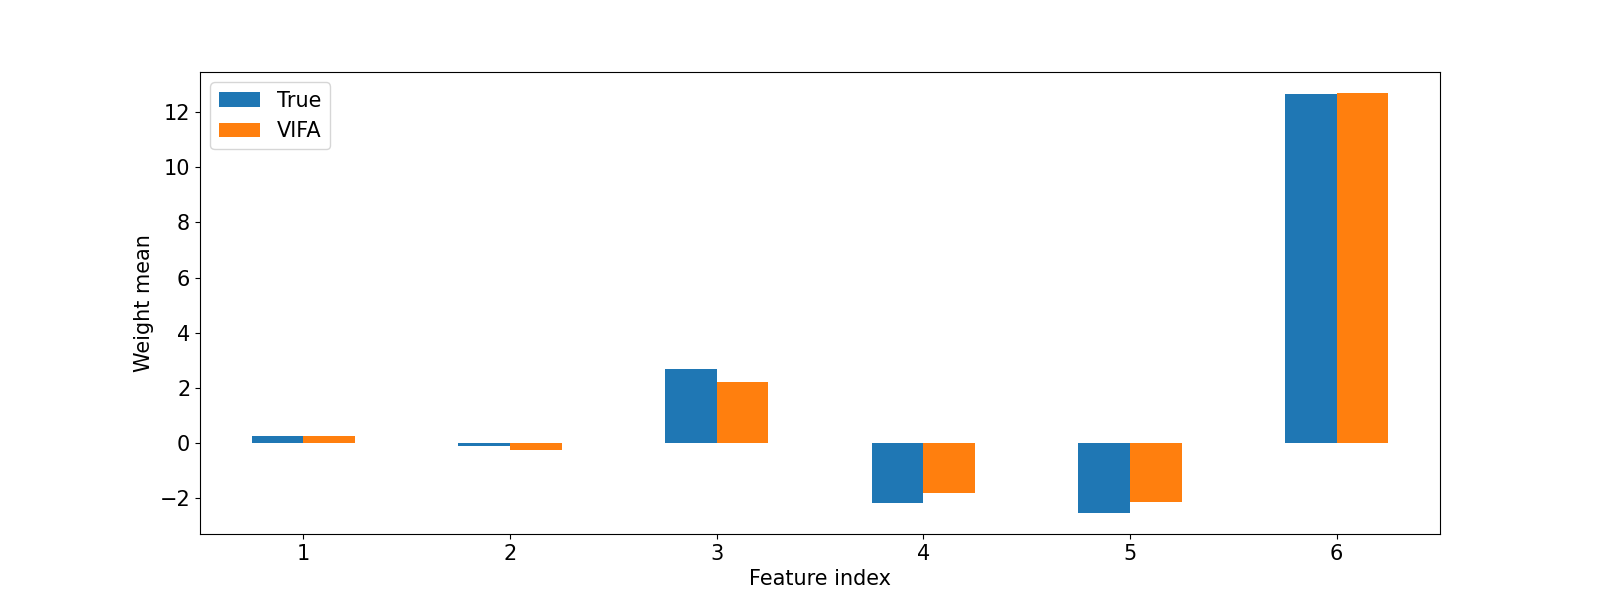
\includegraphics[width=140mm]{plots/yacht_hydrodynamics_posterior_mean.png} \\
		(a) Comparison of true and estimated posterior means \\[6pt] 
		 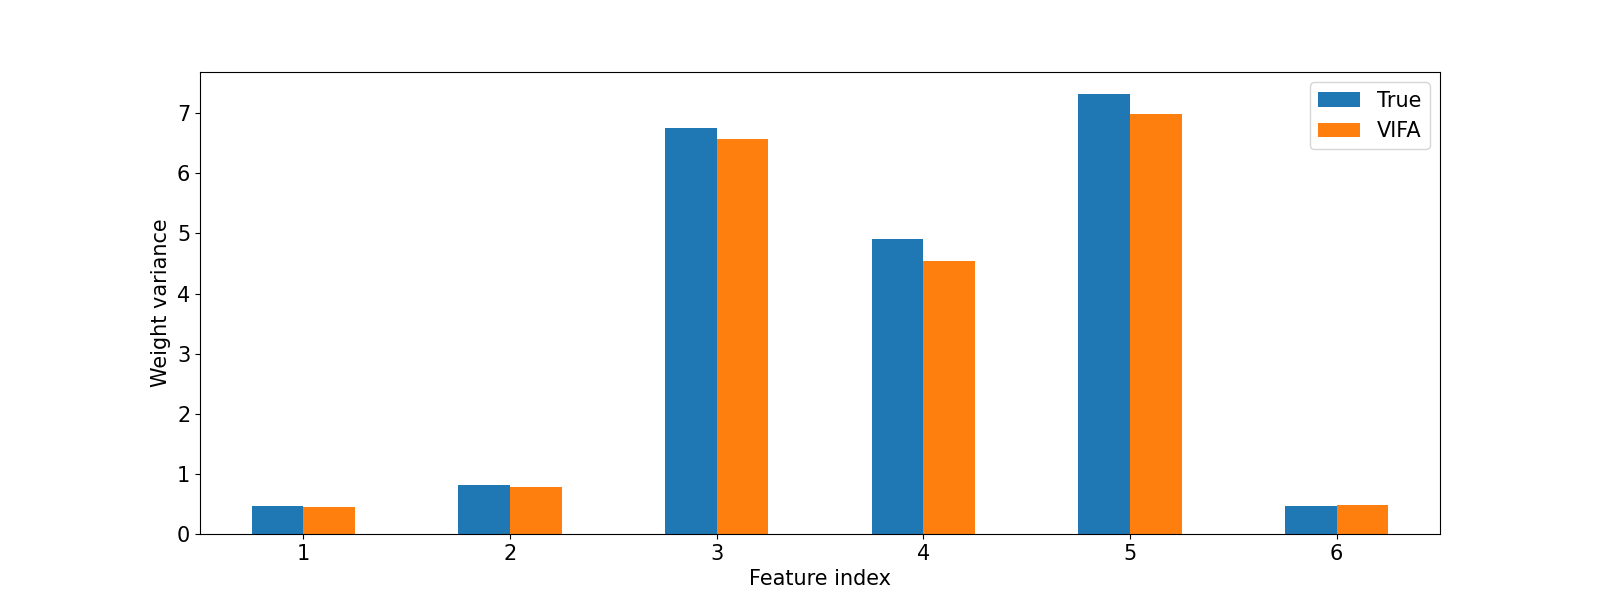
\includegraphics[width=140mm]{plots/yacht_hydrodynamics_posterior_variance.png} \\
		(b) Comparison of true and estimated posterior variances \\[6pt] 
		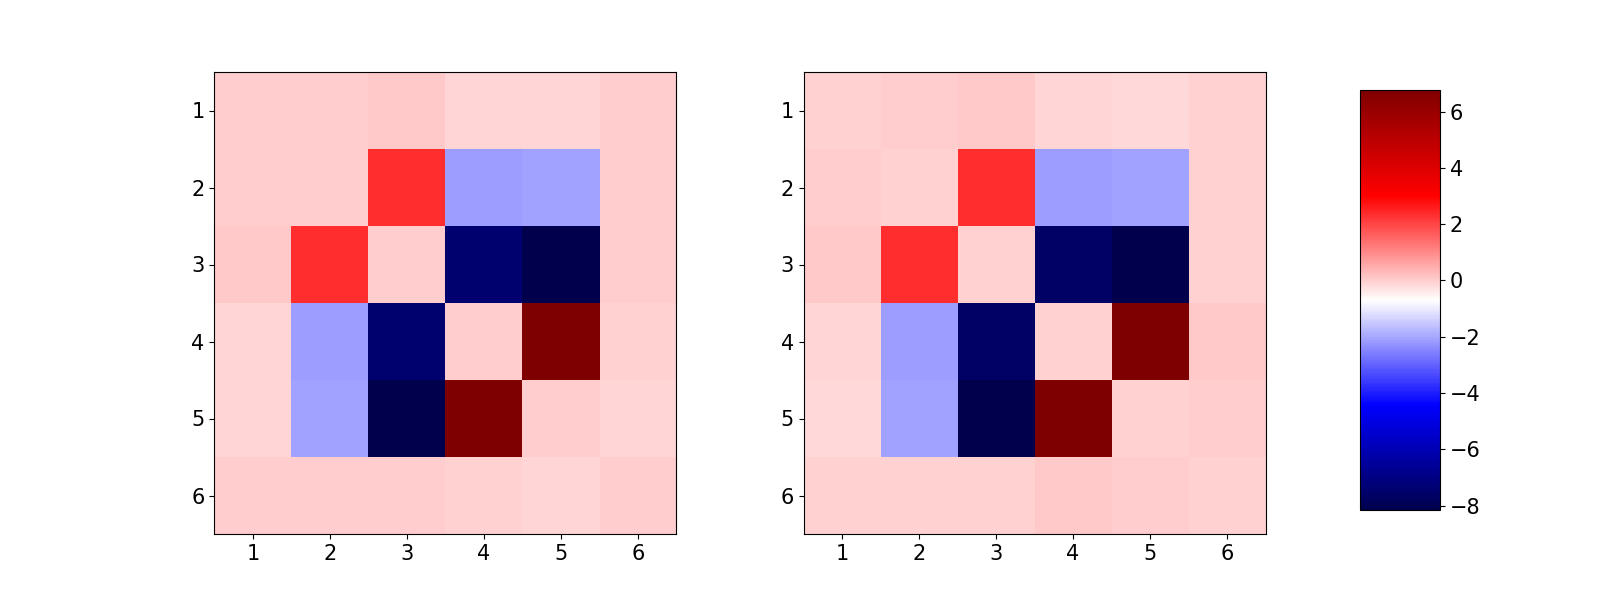
\includegraphics[width=140mm]{plots/yacht_hydrodynamics_posterior_covariance.png} \\
		(c) Comparison of true and estimated posterior covariances \\[6pt] 
	\end{tabular}
	\caption{Comparison of the ground truth posterior of a linear regression model fit to the Yacht Hydrodynamics dataset, and the approximate posterior learned by VIFA. Variances and covariance are plotted separately due to the difference in their magnitude. In plot (c), the diagonal entries of the covariance matrices have been set to zero.}
	\label{fig:posterior_yacht_hydrodynamics}
\end{figure}

\begin{figure}[!htbp] 
	\begin{tabular}{c}
		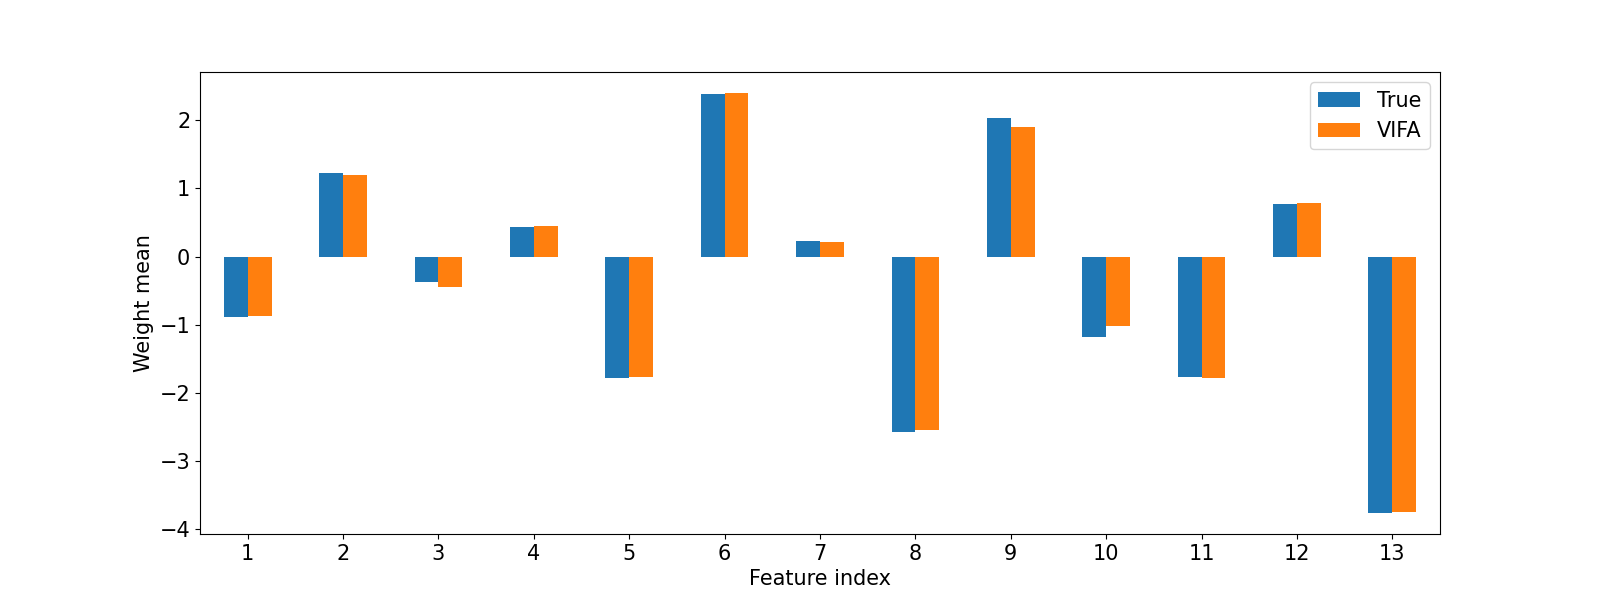
\includegraphics[width=140mm]{plots/boston_housing_posterior_mean.png} \\
		(a) Comparison of true and estimated posterior means \\[6pt] 
		 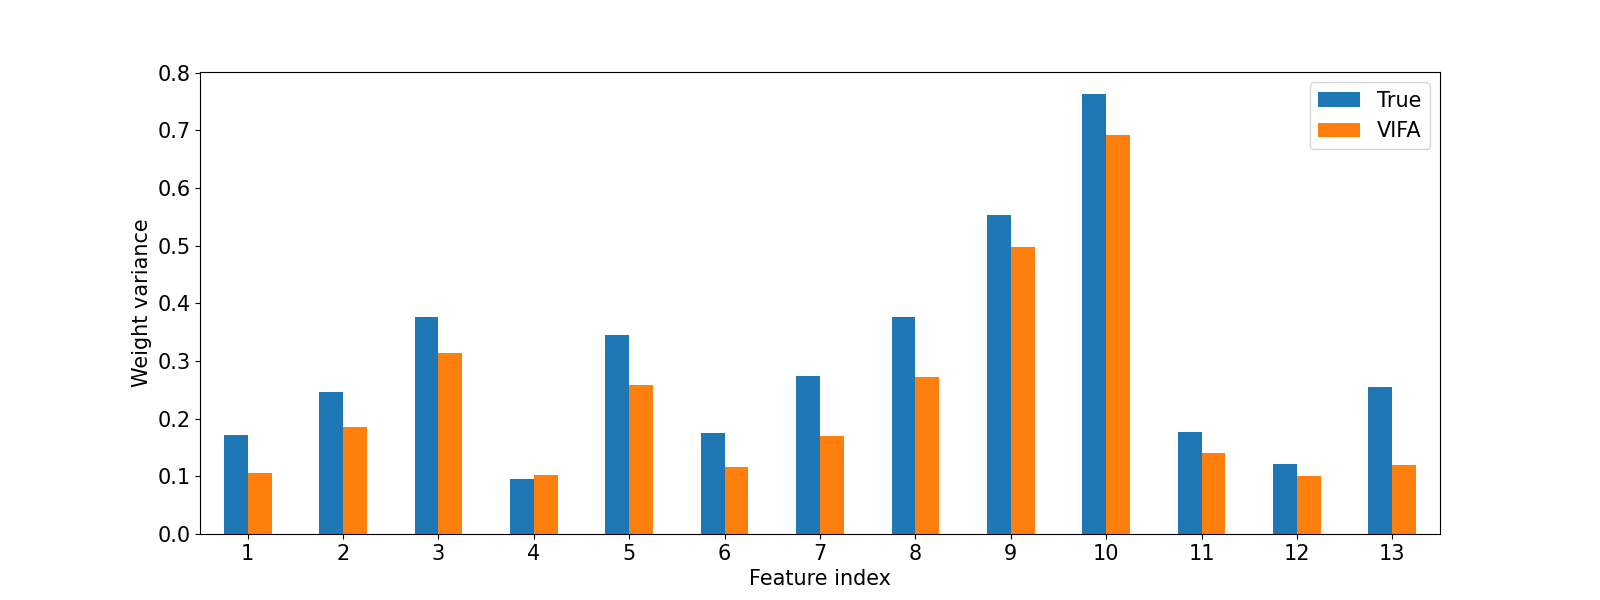
\includegraphics[width=140mm]{plots/boston_housing_posterior_variance.png} \\
		(b) Comparison of true and estimated posterior variances \\[6pt] 
		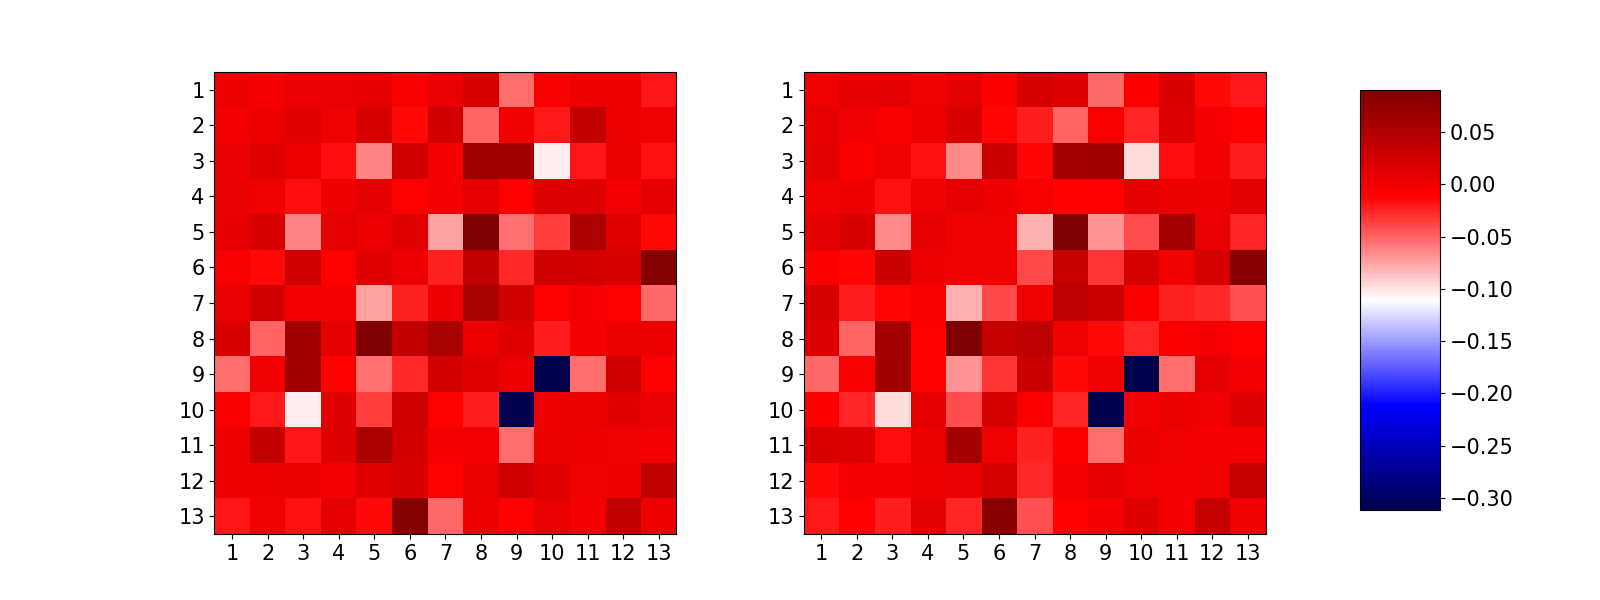
\includegraphics[width=140mm]{plots/boston_housing_posterior_covariance.png} \\
		(c) Comparison of true and estimated posterior covariances \\[6pt] 
	\end{tabular}
	\caption{Comparison of the ground truth posterior of a linear regression model fit to the Boston Housing dataset, and the approximate posterior learned by VIFA. Variances and covariance are plotted separately due to the difference in their magnitude. In plot (c), the diagonal entries of the covariance matrices have been set to zero.}
	\label{fig:posterior_boston_housing}
\end{figure}


\subsection{Neural Network Predictions}\label{sec:uci_nn_predictions}

Given the encouraging results achieved by VIFA when applied to linear regression, the purpose of these experiments is to test VIFA on simple neural networks with a single hidden layer. Unlike linear regression, it is not possible to compute the true posterior distribution of the parameter vector of a non-linear neural network in closed-form. Therefore, the focus of these experiments is on the quality of predictions made by neural networks trained via VIFA in comparison to SLANG. 

The setup for the experiments largely followed the methodology adopted by the authors of SLANG \cite{mishkin2018}. Each neural network had a single hidden layer with 50 rectified linear units (ReLU) and a single, unactivated output. The UCI regression datasets from Table \ref{table:uci_datasets} were used once again. Each dataset was split 20 times into different train and tests sets\footnote{Data splits are available at \texttt{https://github.com/yaringal/DropoutUncertaintyExps}}. For each train-test split, VIFA hyperparameters were tuned using the training data and then the best configuration was evaluated once on the test set. The hyperparameters which were tuned were the learning rate $\eta$, the precision $\alpha$ of the prior and the precision $\beta$ of the additive target noise distribution. As with SLANG, these were optimised via 30 iterations of hyperparameter search, with 5-fold cross-validation performed in each iteration to estimate the marginal log-likelihood. However, while SLANG used Bayesian optimisation, VIFA was tuned via random search to keep things simple. During the search, values for $\eta$, $\alpha$ and $\beta$ were sampled log-uniformly from $[0.01, 0.02]$, $[0.01, 10]$ and $[0.01, 1]$, respectively. To improve numerical stability, any gradients with Frobenius norm greater than 10 were rescaled to have norm of exactly 10. The other hyperparameters were fixed to the same values as SLANG. That is, latent dimension $K=1$, number of epochs $T=120$, mini-batch size $M=10$ and Monte Carlo average size $L=4$. Although vanilla SGD is employed in Algorithm \ref{alg:vi_fa}, a whole host of gradient optimisers can be used in conjunction with VIFA. In this case, the Adam optimiser \cite{kingma2014} was used to perform the gradient updates. Before each training run, the features and target were normalised by subtracting their mean and dividing by their standard deviation. These statistics were computed on training data only, including within each separate fold of cross-validation. When training, the average negative Gaussian log-likelihood was used on line 12 of Algorithm \ref{alg:vi_fa}. When testing, both the average marginal Gaussian log-likelihood and root mean squared error (RMSE) were computed, using a Monte Carlo average size of 100. Full details of how the training loss and test metrics were computed are given in Appendix \ref{app:uci_nn_predictions}. The same experiments were re-run for SLANG\footnote{Using the code available at \texttt{https://github.com/aaronpmishkin/SLANG}} with some minor adjustments to the authors' original setup to allow for a fairer comparison with VIFA. In particular, the Monte Carlo average size when testing and the hyperparameter ranges for $\alpha$ and $\beta$ were adjusted to match those of VIFA. Finally, the VIFA experiments were also run for linear regression models. The only difference being that the hyperparameter range for the learning rate $\eta$ was set to $[0.001, 0.01]$, as this appeared to work better that $[0.01, 0.02]$ during some initial cross-validation runs. 


\subsubsection{Results and Discussion} 

Test metrics for VIFA and SLANG, which were aggregated over the 20 train-test splits, are given in Table \ref{table:neural_nets_uci}. In terms of negative marginal log-likelihood (NMLL), neither algorithm is better than the other on all datasets. For Boston Housing and Concrete Compressive Strength, the mean results for neural networks are essentially the same when standard errors are taken into account. SLANG achieves lower mean NMLL on Yacht Hydrodynamics, but performs extremely poorly on Energy Efficiency with respect to the same metric. It is worth noting that this was caused by a single trial which returned NMLL of $4.04 \times 10^{8}$. This outlier does not affect the median NMLL, which is actually lower than the equivalent value for VIFA. As for mean RMSE, VIFA is the best algorithm on all datasets by some distance. However, SLANG is better on Energy Efficiency and Yacht Hydrodynamics with respect to the median RMSE. The standard errors on the RMSE show that VIFA is very consistent on different train-test splits, whereas the performance of SLANG varies substantially, especially in the case of Energy Efficiency which returned a value of $2.84 \times 10^{4}$ in one trial.  One clear advantage that VIFA has over SLANG is speed. In all experiments involving neural networks, the average runtime of VIFA is roughly half that of SLANG. VIFA generally runs slightly faster when learning a linear regression posterior (although, surprisingly, not in the case of Yacht Hydrodynamics). However, the NMLL and RMSE results indicate that there are non-linear relationships in the datasets which are better captured by the neural network. 

In summary, the choice between VIFA and SLANG depends on the dataset and evaluation metric. However, VIFA certainly has the advantage of being more efficient and appears less sensitive to variations in the training and test data. 

\begin{table}[h!]
	\begin{center}
		\begin{tabular}{|| p{0.10\linewidth} p{0.10\linewidth} p{0.10\linewidth}  p{0.15\linewidth} p{0.15\linewidth} p{0.27\linewidth} ||} 
 			\hline
 			Metric & Statistic & Dataset & VIFA-LR & VIFA-NN & SLANG-NN \\ [0.5ex] 
 			\hline\hline
			NMLL 	& Mean 	& Energy 		& $\mathbf{2.57 \pm 0.02}$ 	& $\mathbf{2.53 \pm 0.02}$ 	& $2.13 \times 10^{7} \pm 2.01 \times 10^{7}$ \\ 	
					&   		& Boston   	& $3.07 \pm 0.12$			& $\mathbf{2.66 \pm 0.06}$ 	& $\mathbf{2.73 \pm 0.06}$ \\ 			
					&   		& Concrete	& $3.77 \pm 0.02$ 			& $\mathbf{3.34 \pm 0.01}$ 	& $\mathbf{3.32 \pm 0.03}$ \\ 			
 					&  		& Yacht    		& $3.65 \pm 0.04$ 			& $2.36 \pm 0.06$ 			& $\mathbf{1.63 \pm 0.04}$ \\
					
					
					& Median	& Energy 		& $2.57$ 					& $2.54$ 					& $\mathbf{1.19}$ \\ 
					& 		& Boston 		& $2.88$	 				& $\mathbf{2.65}$ 			& $2.68$ \\
					& 		& Concrete 	& $3.76$ 					& $3.33$ 					& $\mathbf{3.32}$ \\ 
					& 		& Yacht 		& $3.62$ 					& $2.38$ 					& $\mathbf{1.59}$ \\
 			\hline
			RMSE 	& Mean	& Energy 	 	& $3.07 \pm 0.06$  			& $\mathbf{2.90 \pm 0.06}$ 	& $1.50 \times 10^{3} \pm 1.42 \times 10^{3}$ \\ 
					& 		& Boston 	 	& $4.64 \pm 0.23$ 			& $\mathbf{3.64 \pm 0.23}$ 	& $15.87 \pm 4.36$ \\ 
					& 		& Concrete  	& $10.34 \pm 0.15$ 			& $\mathbf{6.77 \pm 0.09}$ 	& $22.27 \pm 6.64$ \\ 
 					& 		& Yacht 		& $8.96 \pm 0.29$ 			& $\mathbf{2.51 \pm 0.09}$ 	& $8.03 \pm 4.58$ \\ 
				 	& Median	& Energy  		& $3.04$ 					& $2.93$ 					& $\mathbf{1.19}$ \\ 
					& 		& Boston  		& $4.31$ 					& $\mathbf{3.51}$ 			& $6.47$ \\ 
					& 		& Concrete  	& $10.27$ 				& $\mathbf{6.77}$ 			& $9.03$ \\ 
 					& 		& Yacht  		& $9.07$ 					& $2.59$ 					& $\mathbf{1.21}$ \\ 
			\hline			
			Runtime 	& Mean	& Energy 	 	& $\mathbf{22.10}$   		& $22.59$  				& $40.38$  \\ 
			(minutes)	&		& Boston 	 	& $\mathbf{14.78}$			& $16.18$					& $32.97$ \\ 
					&		& Concrete 	& $\mathbf{25.23}$			& $28.41$					& $52.31$ \\ 
 					&		& Yacht 		& $11.78$					& $\mathbf{11.58}$			& $20.61$\\ [1ex] 
			\hline
		\end{tabular}
		\caption{Test results for prediction experiments with UCI regression datasets. Metrics are the average negative marginal log-likelihood (NMLL) and root mean squared error (RMSE). LR and NN refer to linear regression and neural network, respectively. The  results were aggregated over 20 different train-test splits. The mean results for NMLL and RMSE include standard errors. The runtime refers to the total runtime for a single train-test split. That is, 30 rounds of 5-fold cross-validation on the training set followed by fitting the best model to the full training set and evaluating on the test set. All experiments were executed on an Apple M1 chip (2020) with an 8-core CPU and 16GB of RAM. The best results on each row are highlighted in bold.}
		\label{table:neural_nets_uci}
	\end{center}
\end{table}


\chapter{Conclusions}\label{ch:conclusions}

%\section{Final Reminder}

%The body of your dissertation, before the references and any appendices,
%\emph{must} finish by page~40. The introduction, after preliminary material,
%should have started on page~1.
%
%You may not change the dissertation format (e.g., reduce the font
%size, change the margins, or reduce the line spacing from the default
%1.5 spacing). Over length or incorrectly-formatted dissertations will
%not be accepted and you would have to modify your dissertation and
%resubmit.  You cannot assume we will check your submission before the
%final deadline and if it requires resubmission after the deadline to
%conform to the page and style requirements you will be subject to the
%usual late penalties based on your final submission time.

The work in this thesis focused on improving posterior estimation of neural networks. The overall objective was to use properties of FA to overcome some of the limitations of SWAG and SLANG. More specifically, the two main project goals were: (1) implement two online FA algorithms which scale to high-dimensional data, such as the parameter vectors of deep neural networks; (2) implement a model-agnostic VI-based algorithm which learns a FA posterior of a neural network. 

The first two algorithms presented in this thesis (Algorithms \ref{alg:gradient_fa} and \ref{alg:online_em}) are online FA algorithms which can be used to approximate a neural network posterior with a FA model, assuming that representative samples of the posterior can be obtained via some separate procedure. The first method is a stochastic gradient algorithm, whereas the other is based on EM. Crucially, both algorithms are executed online in an iterative fashion and avoid any explicit use of $D \times D$ matrices, ensuring their applicability in the case of very high-dimensional deep neural networks. In the synthetic experiments, the online EM algorithm was shown to be as good as the classic batch SVD algorithm when $10^5$ training samples are available and the conditioning number of the true covariance matrix in not too large. Unfortunately, however, it was not possible to obtain representative samples of the posterior using the approach adopted by SWAG. The results in this thesis suggest that SWAG and its variants do not actually do approximate posterior inference and are perhaps better described as ensemble methods. Nevertheless, the online FA algorithms, and in particular online EM, are useful in their own right and could potentially still contribute to Bayesian deep learning if combined with better posterior sampling methods. 

Currently, however, the more direct VIFA algorithm (Algorithm \ref{alg:vi_fa}) appears a much better approach to posterior estimation. This was demonstrated in the experiments involving linear regressions models, fit to both synthetic and real datasets. In all cases, VIFA was able to learn a good approximation of the true posterior covariance. Moreover, VIFA also achieved encouraging results in the neural network predictions experiments in comparison to SLANG, in terms of RMSE, marginal likelihood and runtime. 

There are some notable similarities between VIFA and SLANG. Both are VI-based approaches to neural network posterior estimation and both use a low-rank plus diagonal approximation of a $D \times D$ matrix to make the computation tractable - VIFA approximates the posterior covariance whereas SLANG approximates its inverse. Although they are both online gradient-based algorithms, VIFA uses vanilla gradients whereas SLANG uses natural gradients. While in theory natural gradient methods are preferable when optimising the parameters of a distribution, in practice this leads to undesirable features. In particular, the SLANG update uses a randomised eigen-decomposition algorithm which requires the back-propagated gradients of individual training examples. This is problematic, since an efficient algorithm requires a separate implementation of back-propagation for each different type of neural network layer. Perhaps the biggest advantage of VIFA is that it only requires the gradient of the average negative log-likelihood of a mini-batch of training examples. This is easy to obtain using standard automatic differentiation tools in deep learning frameworks such as PyTorch \cite{paszke2019}. Hence, VIFA is model-agnostic and can be applied to any neural network architecture with no extra effort. In this regard, VIFA is a much more practical algorithm that SLANG, as well as being twice as fast.

Given the positive results achieved by VIFA in this thesis, a good next step would be to apply the algorithm to very high-dimensional deep neural networks. VIFA was implemented with this in mind. The fact that Algorithm \ref{alg:vi_fa} uses only basic matrix operations and avoids any explicit use of $D \times D$ matrices means that it should be applicable to deep models with millions or even billions of parameters. Running prediction experiments similar to those in Section \ref{sec:uci_nn_predictions} but with bigger datasets and bigger models would be an excellent test of the scalability of VIFA. It would also be interesting to include classification datasets in these experiments, since this thesis only dealt with regression. VIFA can be applied in this scenario by simply changing the likelihood distribution from Gaussian to multinomial. Finally, the claim that VIFA is model-agnostic should be put to the test in practice. All experiments in this thesis involved either linear regression models or fully-connected neural networks. Further experiments should be executed to test the predictions made by VIFA when applied to other architectures, such as those containing convolutional, recurrent and transformer layers.


\bibliographystyle{plain}
\bibliography{main}

% You can include appendices like this:
 \appendix
 
 \chapter{Supplementary Derivations}
 
 \section{Linear Regression Posterior}\label{app:bayesian_linear_regression_posterior}
 
This section completes the derivation of the linear regression posterior from Section \ref{sec:bayesian_lr}. Recall from Equation (\ref{eqn:linear_regression_log_likelihood}) that
\begin{align}
\begin{split}
	\log p(\mathcal{D} | \theta) 
	& = - \frac{\beta}{2} \sum_{n=1}^N \big(y_n - \theta^\intercal \matr{x}_n \big)^2 
	+ \frac{N}{2} \log \beta
	+ \text{constant}.
\end{split}
\end{align}
Also, applying the logarithm to the prior in Equation (\ref{eqn:linear_regression_prior}),
\begin{align}
\begin{split}
	\log p(\theta) 
	& = \frac{D}{2} \log \frac{\alpha}{2\pi} - \frac{\alpha}{2} \theta^\intercal \theta \\
	& = -\frac{\alpha}{2} \theta^\intercal \theta + \frac{D}{2} \log \alpha + \text{constant}.
\end{split}
\end{align}
Suppose that the prior precision $\alpha$ and the noise precision $\beta$ are fixed. Then it follows from Bayes' rule that
\begin{align}\label{eqn:linear_regression_log_posterior}
\begin{split}
	\log p(\theta | \mathcal{D}) 
	& = \log \frac{p(\mathcal{D} | \theta) p(\theta)}{p(\mathcal{D})} \\
	& = \log p(\mathcal{D} | \theta) + \log p(\theta) - \log p(\mathcal{D}) \\
	& = -\frac{\beta}{2} \sum_{n=1}^N \big(y_n - \theta^\intercal \matr{x}_n \big)^2 
	-\frac{\alpha}{2} \theta^\intercal \theta 
	+ \text{constant} \\
	& = -\frac{\beta}{2} \sum_{n=1}^N\big( y_n^2 - 2 y_n \theta^\intercal \matr{x}_n + (\theta^\intercal \matr{x}_n)^2 \big)
	-\frac{\alpha}{2} \theta^\intercal \theta
	+ \text{constant} \\
	& = -\frac{\beta}{2} \sum_{n=1}^N y_n^2
	+ \beta \sum_{n=1}^N y_n \theta^\intercal \matr{x}_n
	-\frac{\beta}{2} \sum_{n=1}^N \theta^\intercal \matr{x}_n \matr{x}_n^\intercal \theta
	-\frac{\alpha}{2} \theta^\intercal \theta
	+ \text{constant} \\
	& = \Big(\beta \sum_{n=1}^N y_n \matr{x}_n \Big)^\intercal \theta 
	-\frac{1}{2} \theta^\intercal \Big( \alpha \matr{I} + \beta \sum_{n=1}^N \matr{x}_n \matr{x}_n^\intercal \Big) \theta 
	+ \text{constant} \\
	& = \matr{b}^\intercal \theta 
	- \frac{1}{2} \theta^\intercal \matr{A} \theta 
	+ \text{constant},
\end{split}
\end{align}
where 
\begin{equation}
	\matr{A} = \alpha \matr{I} + \beta \sum_{n=1}^N \matr{x}_n \matr{x}_n^\intercal
	\quad \text{and} \quad 
	\matr{b} = \beta \sum_{n=1}^N y_n \matr{x}_n.
\end{equation}
Now, using a result from \cite{barber2007} to complete the square of Equation (\ref{eqn:linear_regression_log_posterior}),
\begin{align}
\begin{split}
	\log p(\theta | \mathcal{D}) 
	& = \matr{b}^\intercal \theta 
	- \frac{1}{2} \theta^\intercal \matr{A} \theta 
	+ \text{constant} \\
	& = -\frac{1}{2} \big(\theta - \matr{A}^{-1} \matr{b} \big)^\intercal \matr{A} \big(\theta - \matr{A}^{-1} \matr{b} \big)
	+ \frac{1}{2} \matr{b}^\intercal \matr{A}^{-1} \matr{b}
	+ \text{constant} \\
	& = -\frac{1}{2} \big(\theta - \matr{A}^{-1} \matr{b} \big)^\intercal \matr{A} \big(\theta - \matr{A}^{-1} \matr{b} \big)
	+ \text{constant} \\
	& = -\frac{1}{2} \big(\theta - \matr{m} \big)^\intercal \matr{S}^{-1} \big(\theta - \matr{m} \big)
	+ \text{constant},
\end{split}
\end{align}
where
\begin{equation}
	\matr{m} = \matr{A}^{-1} \matr{b}
	\quad \text{and} \quad 
	\matr{S} = \matr{A}^{-1}.
\end{equation}
Hence, the posterior distribution of $\theta$ is 
\begin{align}
\begin{split}
	p(\theta | \mathcal{D}) = \mathcal{N}(\matr{m}, \matr{S}).
\end{split}
\end{align}

 \chapter{Supplementary Algorithmic Details}

\section{Partial Derivatives for Online SGA Factor Analysis}\label{app:online_fa_sga_derivatives}

This section presents a full derivation of the partial derivatives, $\nabla_{\matr{F}, \Psi} \log p(\theta_t | \matr{F}, \Psi)$, given in Equations (\ref{eqn:derivatives_wrt_F}) and (\ref{eqn:derivatives_wrt_Psi}) for the online SGA FA algorithm. Recall from Section \ref{sec:gradient_fa} that the goal is to compute the expected value of 
\begin{align}\label{eqn:log_fa_cond_dist_app}
\begin{split}
	\log p(\theta_t | \matr{h}_t, \matr{F}, \Psi)
	& = -\frac{1}{2} (\matr{d}_t - \matr{Fh}_t)^\intercal \Psi^{-1} (\matr{d}_t - \matr{Fh}_t) - \frac{1}{2} \log |\Psi| - \frac{D}{2} \log 2\pi
\end{split}
\end{align}
over the distribution $p(\matr{h}_t | \theta_t, \matr{F}, \Psi)$, where $\matr{d}_t = \theta_t - \theta_{\text{SWA}}$.

\subsection{Partial derivatives with respect to $\matr{F}$}

From \cite{petersen2012}, for any symmetric matrix $\matr{W}$,
\begin{equation}
	\nabla_{\matr{A}} (\matr{x} - \matr{As})^\intercal \matr{W} (\matr{x} - \matr{As}) = -2 \matr{W} (\matr{x} - \matr{As}) \matr{s}^\intercal.
\end{equation}
Hence, differentiating Equation (\ref{eqn:log_fa_cond_dist_app}) with respect to $\matr{F}$ gives
\begin{equation}
	\nabla_{\matr{F}} \log p(\theta_t | \matr{h}_t, \matr{F}, \Psi)
	= \Psi^{-1} (\matr{d}_t - \matr{Fh}_t) \matr{h}_t^\intercal.
\end{equation}
It then follows that $\nabla_{\matr{F}} \log p(\theta_t | \matr{F}, \Psi)$ is the expected value of $\Psi^{-1} (\matr{d}_t - \matr{Fh}_t) \matr{h}_t^\intercal$ over the distribution $p(\matr{h}_t | \theta_t, \matr{F}, \Psi)$. Letting $\E[\cdot]$ denote $\E_{p(\matr{h}_t | \theta_t, \matr{F}, \Psi)}[\cdot]$ to simplify the notation, 
\begin{align}\label{eqn:expected_derivatives_wrt_F}
\begin{split}
	\nabla_{\matr{F}} \log p(\theta_t | \matr{F}, \Psi) 
	& = \E \big[ \Psi^{-1} (\matr{d}_t - \matr{Fh}_t) \matr{h}_t^\intercal \big] \\
	%& = \Psi^{-1} \big(\E \big[ \matr{d}_t \matr{h}_t^\intercal \big] 
	%- \E \big[ \matr{Fh}_t \matr{h}_t^\intercal \big] \big) \\
	& = \Psi^{-1}\big( \matr{d}_t \E \big[ \matr{h}_t^\intercal \big] 
	- \matr{F}  \E \big[ \matr{h}_t \matr{h}_t^\intercal \big]\big).
\end{split}
\end{align} 
From the E-step of the EM algorithm for FA in \cite{barber2007}, $p(\matr{h}_t | \theta_t, \matr{F}, \Psi) \propto \mathcal{N}(\matr{m}_t, \Sigma)$, where
\begin{equation}
	\Sigma = (\matr{I} + \matr{F}^\intercal \Psi^{-1} \matr{F})^{-1}
	\quad \text{and} \quad \matr{m}_t = \Sigma \matr{F}^\intercal \Psi^{-1} \matr{d}_t.
\end{equation}
Hence, using the identities for vector and matrix expectations from \cite{petersen2012}, 
\begin{equation}\label{eqn:expected_value_h_hh}
	\E \big[ \matr{h}_t^\intercal \big] = \matr{m}_t^\intercal \quad \text{and} \quad \E \big[ \matr{h}_t \matr{h}_t^\intercal \big] = \Sigma + \matr{m}_t \matr{m}_t^\intercal.
\end{equation}
Finally, substituting the expectations in Equation (\ref{eqn:expected_value_h_hh}) into Equation (\ref{eqn:expected_derivatives_wrt_F}), 
\begin{align}
\begin{split}
	\nabla_{\matr{F}} \log p(\theta_t | \matr{F}, \Psi) 
	& = \Psi^{-1} \big(\matr{d}_t \matr{m}_t^\intercal - \matr{F}  (\Sigma + \matr{m}_t \matr{m}_t^\intercal)\big).
\end{split}
\end{align} 

\subsection{Partial derivatives with respect to $\Psi$}

In order to differentiate Equation (\ref{eqn:log_fa_cond_dist_app}) with respect to $\Psi$, it helps to use the fact that $\Psi$ is diagonal. First consider $\matr{X}^{-1} = \diag\big(\frac{1}{x_1}, \dots, \frac{1}{x_D}\big)$ and $\matr{a} = (a_1, \dots, a_D)^\intercal$. Then 
\begin{equation}\label{eqn:aXa}
	\matr{a}^\intercal \matr{X}^{-1} \matr{a} = \sum_{d=1}^D \frac{a_d^2}{x_d},
\end{equation}
and so
\begin{equation}
	\frac{\partial}{\partial x_d} \matr{a}^\intercal \matr{X}^{-1} \matr{a} = \frac{-a_d^2}{x_d^2}
\end{equation}
for $d=1, \dots, D$. Since the partial derivatives of Equation (\ref{eqn:aXa}) with respect to the off-diagonal entries of $\matr{X}$ are zero, 
\begin{align}\label{eqn:derivatives_diag_qaud_form}
\begin{split}
	\nabla_\matr{X} (\matr{a}^\intercal \matr{X}^{-1} \matr{a}) 
	& = \diag\Big({\frac{-a_1^2}{x_1^2}, \dots, \frac{-a_D^2}{x_D^2}}\Big) \\
	& = -\diag\big(\diag(\matr{X}^{-2}) \odot \matr{a}^2\big),
\end{split}
\end{align}  
where $\odot$ denotes the element-wise matrix product (with broadcasting, if applicable) and the square of the vector is applied element-wise. Also, when applied to a $D$-length vector, $\diag(\cdot)$ represents the $D \times D$ diagonal matrix with the vector on its diagonal, and when applied to a $D \times D$ matrix, $\diag(\cdot)$ represents the $D$-length vector consisting of the diagonal entries of the matrix. Substituting $\matr{X} = \Psi$ and $\matr{a} = \matr{d}_t - \matr{Fh}_t$ into Equation (\ref{eqn:derivatives_diag_qaud_form}),
\begin{equation}\label{eqn:derivatives_wrt_Psi_1}
	\nabla_\Psi (\matr{d}_t - \matr{Fh}_t)^\intercal \Psi^{-1} (\matr{d}_t - \matr{Fh}_t) 
	= -\diag\big(\diag(\Psi^{-2}) \odot (\matr{d}_t - \matr{Fh}_t)^2\big).
\end{equation}
Also, using the identity $\nabla_\matr{X} \log |\matr{X}| = \matr{X}^{-\intercal}$ from \cite{petersen2012} and the fact that $\Psi^{-\intercal} = \Psi^{-1}$, 
\begin{equation}\label{eqn:derivatives_wrt_Psi_2}
	\nabla_\Psi \log |\Psi|
	= \Psi^{-1}.
\end{equation}
Hence, the partial derivatives of Equation (\ref{eqn:log_fa_cond_dist_app}) with respect to $\Psi$ are
\begin{equation}
	\nabla_{\Psi} \log p(\theta_t | \matr{h}_t, \matr{F}, \Psi)
	= \frac{1}{2} \diag\big(\diag(\Psi^{-2}) \odot (\matr{d}_t - \matr{Fh}_t)^2\big) - \frac{1}{2}\Psi^{-1}.
\end{equation}
Again, letting $\E[\cdot]$ denote $\E_{p(\matr{h}_t | \theta_t, \matr{F}, \Psi)}[\cdot]$, it follows that
\begin{align}\label{eqn:expected_gradient}
\begin{split}
	2 \cdot \nabla_{\Psi} \log p(\theta_t | \matr{F}, \Psi) 
	& = \E \big[ \diag\big(\diag(\Psi^{-2}) \odot (\matr{d}_t - \matr{Fh}_t)^2\big) - \Psi^{-1} \big] \\
	%& = \diag\Big(\E \big[\diag(\Psi^{-2}) \odot (\matr{d}_t - \matr{Fh}_t)^2\big]\Big) - \E \big[ \Psi^{-1} \big] \\
	& = \diag\Big(\diag(\Psi^{-2}) \odot \E \big[(\matr{d}_t - \matr{Fh}_t)^2\big]\Big) - \Psi^{-1}.
\end{split}
\end{align} 
Now, expanding the expectation inside Equation (\ref{eqn:expected_gradient}) and substituting in the expressions from Equation (\ref{eqn:expected_value_h_hh}),
\begin{align}\label{eqn:expected_gradient_d_Fh}
\begin{split}
	\E \big[(\matr{d}_t - \matr{Fh}_t)^2\big] 
	& = \E \big[\matr{d}_t \odot \matr{d}_t \big] - 2\E \big[ \matr{d}_t \odot (\matr{Fh}_t) \big] + \E \big[ (\matr{Fh}_t) \odot (\matr{Fh}_t) \big] \\
	& = \matr{d}_t \odot \matr{d}_t - 2\matr{d}_t \odot \big(\matr{F} \E \big[ \matr{h}_t \big]\big) + \E \big[ \diag(\matr{F}\matr{h}_t \matr{h}_t^\intercal  \matr{F}^\intercal) \big] \\
	%& = \matr{d}_t \odot \matr{d}_t - 2\matr{d}_t \odot (\matr{F} \matr{m}_t) + \diag\big(\E \big[ \matr{F}\matr{h}_t \matr{h}_t^\intercal  \matr{F}^\intercal \big]\big) \\
	& = \matr{d}_t \odot \matr{d}_t - 2\matr{d}_t \odot (\matr{F} \matr{m}_t) + \diag\big( \matr{F} \E \big[ \matr{h}_t \matr{h}_t^\intercal \big] \matr{F}^\intercal \big) \\
	& = \matr{d}_t \odot \matr{d}_t - 2\matr{d}_t \odot (\matr{F} \matr{m}_t) + \diag\big( \matr{F} (\Sigma + \matr{m}_t \matr{m}_t^\intercal) \matr{F}^\intercal \big).
\end{split}
\end{align} 
Finally, substituting Equation (\ref{eqn:expected_gradient_d_Fh}) into Equation (\ref{eqn:expected_gradient}) and rearranging, 
\begin{align}
\begin{split}%\label{eqn:derivatives_wrt_Psi}
	\nabla_{\Psi} \log p(\theta_t | \matr{F}, \Psi) 
	& = \diag\Bigg(\frac{1}{2} \diag(\Psi^{-2}) \odot \Big(\matr{d}_t \odot \matr{d}_t - 2\matr{d}_t \odot (\matr{F} \matr{m}_t) \\
	& \quad + \diag\big( \matr{F} (\Sigma + \matr{m}_t \matr{m}_t^\intercal) \matr{F}^\intercal \big) \Big) \Bigg)
	 - \frac{1}{2} \Psi^{-1}.
\end{split}
\end{align} 

\section{E-step and M-step for Online EM Factor Analysis}\label{app:online_em_steps}

The batch EM algorithm for FA was introduced in Section \ref{sec:online_em}. This section gives more details about the E-step and M-step and explains how these can be modified for an online version of the algorithm.

\subsection{E-step}

In the batch E-step, $\matr{F}$ and $\Psi$ are held fixed and the expression
\begin{equation}\label{eqn:EM_objective}
	- \sum_{t=1}^T \E_{q(\matr{h}_t | \theta_t)} \big[\log q(\matr{h}_t | \theta_t)\big]
	+ \sum_{t=1}^T \E_{q(\matr{h}_t | \theta_t)} \big[\log p(\matr{h}_t, \theta_t | \matr{F}, \Psi)\big]
\end{equation}
from Equation (\ref{eqn:EM_bound}) is maximised with respect to the variational distributions $q(\matr{h}_t | \theta_t)$, $t=1,\dots,T$. From \cite{barber2007}, the optimal variational distributions are 
\begin{equation}
	q(\matr{h}_t | \theta_t) = p(\matr{h}_t | \theta_t, \matr{F}, \Psi)  \propto \mathcal{N}(\matr{m}_t, \Sigma), 
\end{equation}
where $\matr{m}_t$ and $\Sigma$ are given in Equation (\ref{eqn:efficient_m_and_sigma}). Note that this optimisation can be performed separately for each $\theta_t$ as it is sampled, using the estimates of $\matr{F}$ and $\Psi$ on iteration $t$. However, in batch EM \emph{all} $q(\matr{h}_t | \theta_t)$ are updated on every iteration. This is clearly not possible in an online algorithm which discards $\theta_t$ before sampling $\theta_{t + 1}$. Therefore, as a compromise, in the online version each $q(\matr{h}_t | \theta_t)$ can be computed once only, on iteration $t$, and held fixed thereafter. The only other detail is that the batch algorithm uses $\theta_{\text{SWA}}$ to compute $\matr{m}_t$. As $\theta_{\text{SWA}}$ is not available during training, it can be replaced by the running average of the neural network's parameter vectors, as in Algorithm \ref{alg:gradient_fa}.


\subsection{M-step}

In the batch M-step, the variational distributions $q(\matr{h}_t | \theta_t)$, $t=1,\dots,T$, are fixed and the expression in Equation (\ref{eqn:EM_objective}) is maximised with respect to $\matr{F}$ and $\Psi$. From \cite{barber2007}, the optimal values are 
\begin{equation}
	\matr{F} = \matr{A}\matr{H}^{-1}, 
\end{equation}
where $\matr{d}_t = \theta_t - \theta_{\text{SWA}}$,
\begin{equation}
	\matr{A} = \frac{1}{T} \sum_{t=1}^T \matr{d}_t \matr{m}_t^\intercal \quad \text{and} \quad 
	\matr{H} = \Sigma + \frac{1}{T} \sum_{t=1}^T \matr{m}_t \matr{m}_t^\intercal,
\end{equation}
and
\begin{equation}
	\Psi = \text{diag}\Bigg(\text{diag}\Bigg( \frac{1}{T} \sum_{t=1}^T \matr{d}_t \matr{d}_t^\intercal - 2\matr{FA}^\intercal + \matr{FHF}^\intercal \Bigg)\Bigg).
\end{equation}
Note that this optimisation involves summing over $t=1,\dots,T$. Moreover, on each iteration all components of the sums are updated using the latest values of $\matr{m}_t$, $t=1,\dots,T$. As in the E-step, updating all components is not possible in an online algorithm. Therefore, in the online version these sums must instead be updated incrementally. This incremental approach was described in Section \ref{sec:online_em_practical}.


 \chapter{Supplementary Experiment Details}
 
 \section{Online Factor Analysis}\label{app:online_fa}
 
This section provides more details and results for the online FA experiments in Section \ref{ch:online_fa_experiments}. Recall that synthetic FA models were generated for these experiments. The pseudocode in Algorithm \ref{alg:generate_fa} shows exactly how this was done.
  \begin{algorithm}[!htbp] 
	\caption{Generate a Factor Analysis Model}
	\label{alg:generate_fa}
	\begin{algorithmic}[1]
		\Require{Observation dimension $D$, latent dimension $K$, spectrum range $[a, b]$} 
		\State Generate $\matr{c} \in \R^D$ by sampling entries independently from $\mathcal{N}(0, 1)$
		\State Generate $\matr{A} \in \R^{D \times D}$ by sampling entries independently from $\mathcal{N}(0, 1)$
		\State $\matr{M} \leftarrow \matr{A} \matr{A}^\intercal$
		\State Compute the $K$ eigenvectors, $\matr{v}_1, \dots, \matr{v}_K \in \R^D$, corresponding to the $K$ largest eigenvalues of $\matr{M}$
		\State Construct the matrix $\matr{V}_K \in \R^{D \times K}$ with columns $\matr{v}_1, \dots, \matr{v}_K$
		\State Generate $\matr{s}^2 \in \R^D$ by sampling entries independently from $\mathcal{U}(a, b)$
		\State $\matr{F} \leftarrow \matr{V}_K \odot \sqrt{\matr{s}^2}$ (with broadcasting and square root applied element-wise)
		\State $s_{max} \leftarrow \max({\matr{s}^2})$ (largest element of ${\matr{s}^2}$)
		\State Generate $\psi \in \R^D$ by sampling entries independently from $\mathcal{U}(0, s_{max}) $
		\State $\Psi \leftarrow \text{diag}(\psi)$
		\State \Return $\matr{c}, \matr{F}, \Psi$	
	\end{algorithmic}
\end{algorithm}

Recall that Figure \ref{fig:fa_covar_distance} shows the relative distance of the estimated FA covariance matrices from the true covariance matrix as a function of the number of samples used to learn the models. Table \ref{table:fa_covar_distance} contains the numerical results for 100,000 training samples. That is, the results corresponding to the right-most points in each plot.
\begin{table}[h!]
	\begin{center}
		\begin{tabular}{|| p{0.12\linewidth} p{0.20\linewidth} p{0.20\linewidth} p{0.20\linewidth} p{0.20\linewidth} ||} 
 			\hline
 			Obs. Dim & Spectrum Range & Batch SVD & Online EM & Online SGA \\ [0.5ex] 
 			\hline\hline
			100 	& $[1, 10]$ 	& $0.0454 \pm 0.0077$ 	& $0.0399 \pm 0.0058$	& $0.0426 \pm 0.0005$ \\ 
				& $[1, 100]$ 	& $0.0631 \pm 0.0073$ 	& $0.0613 \pm 0.0057$ 	& $0.1309 \pm 0.0038$ \\ 
				& $[1, 1000]$	& $0.0608 \pm 0.0087$ 	& $0.1767 \pm 0.0037$ 	& $0.2350 \pm 0.0046$ \\ 
			\hline
			1000	& $[1, 10]$ 	& $0.0204 \pm 0.0010$ 	& $0.0207 \pm 0.0003$ 	& $0.0546 \pm 0.0009$ \\ 
				& $[1, 100]$ 	& $0.0217 \pm 0.0011$ 	& $0.0238 \pm 0.0013$ 	& $0.0472 \pm 0.0008$ \\ 
				& $[1, 1000]$ 	& $0.0218 \pm 0.0011$ 	& $0.0501 \pm 0.0016$ 	& $0.0945 \pm 0.0024$ \\ [1ex] 
			\hline
		\end{tabular}
		\caption{The relative distance of the estimated FA covariance matrix from the true covariance matrix when 
		the number of training samples is 100,000. Each result is the mean value over ten trials with different random seeds, along with standard errors. These results correspond to the right-most points in the plots in Figure \ref{fig:fa_covar_distance}.}
		\label{table:fa_covar_distance}
	\end{center}
\end{table}

Figure \ref{fig:fa_wasserstein} shows the scaled 2-Wasserstein distance between the Gaussian distribution defined by each estimated FA model and the Gaussian distribution defined by the true FA model, for the same combinations of observation dimension, latent dimension, spectrum range and sample size as Figure \ref{fig:fa_covar_distance}. The numerical results for the case of 100,000 training samples are given in table \ref{table:fa_wasserstein}.
\begin{figure}[!htbp] 
	\begin{tabular}{cc}
		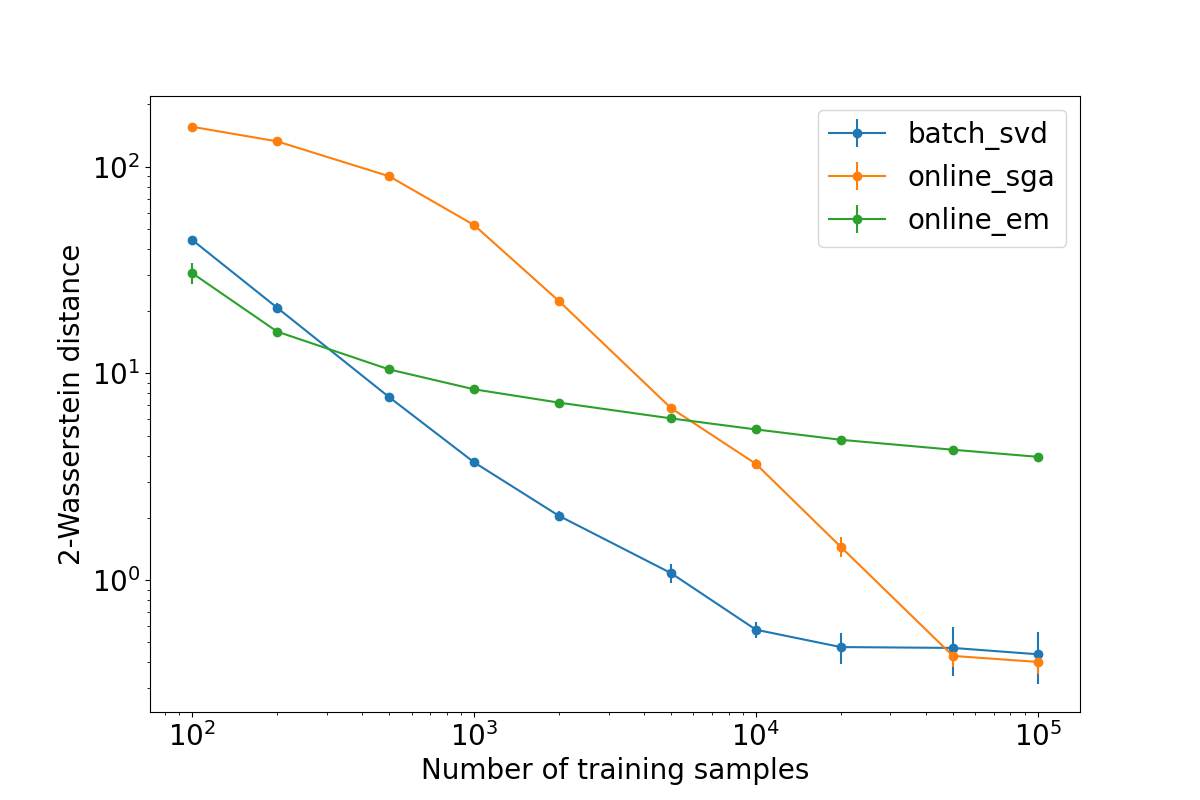
\includegraphics[width=70mm]{plots/online_fa_wasserstein__observation_dim=100__latent_dim=10__spectrum_min=1__spectrum_max=10.png}
		& 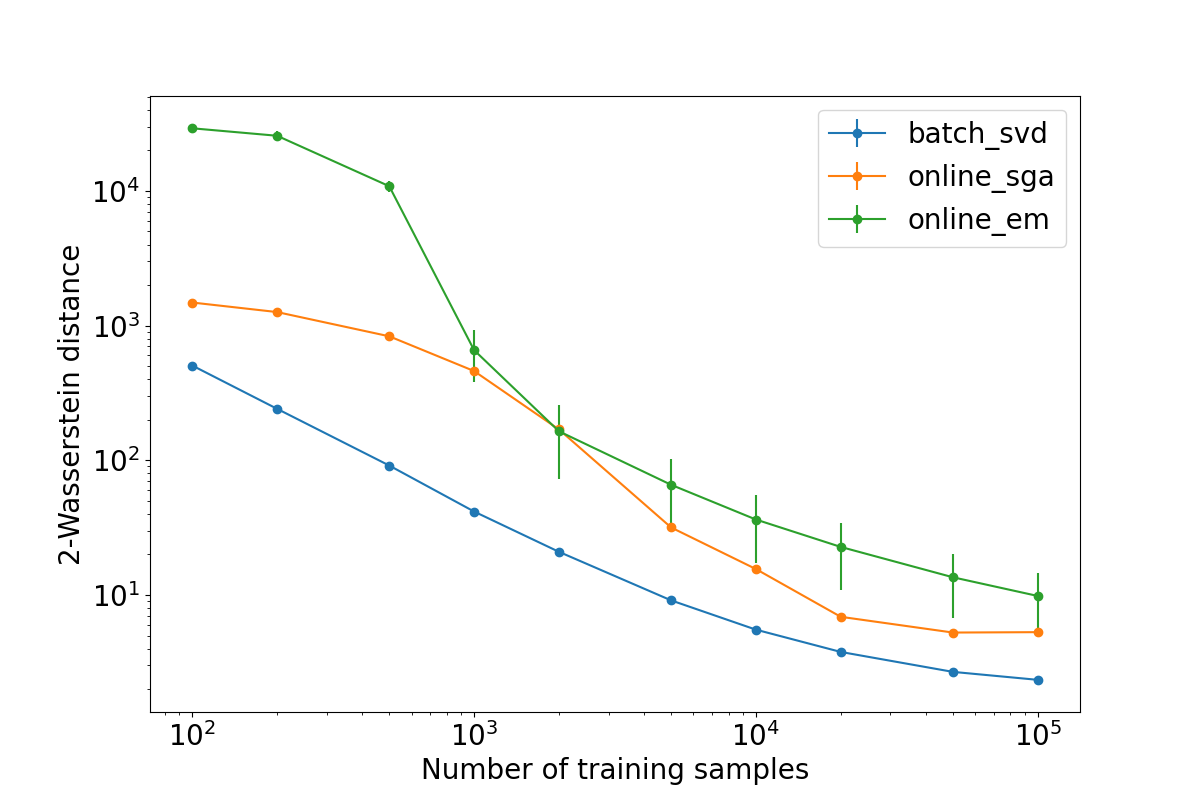
\includegraphics[width=70mm]{plots/online_fa_wasserstein__observation_dim=1000__latent_dim=10__spectrum_min=1__spectrum_max=10.png} \\
		(a) $D=100$, $K=10$, $\matr{s}^2 \sim \mathcal{U}(1, 10)$ 
		 & (b) $D=1000$, $K=10$, $\matr{s}^2 \sim \mathcal{U}(1, 10)$\\[6pt] 
		 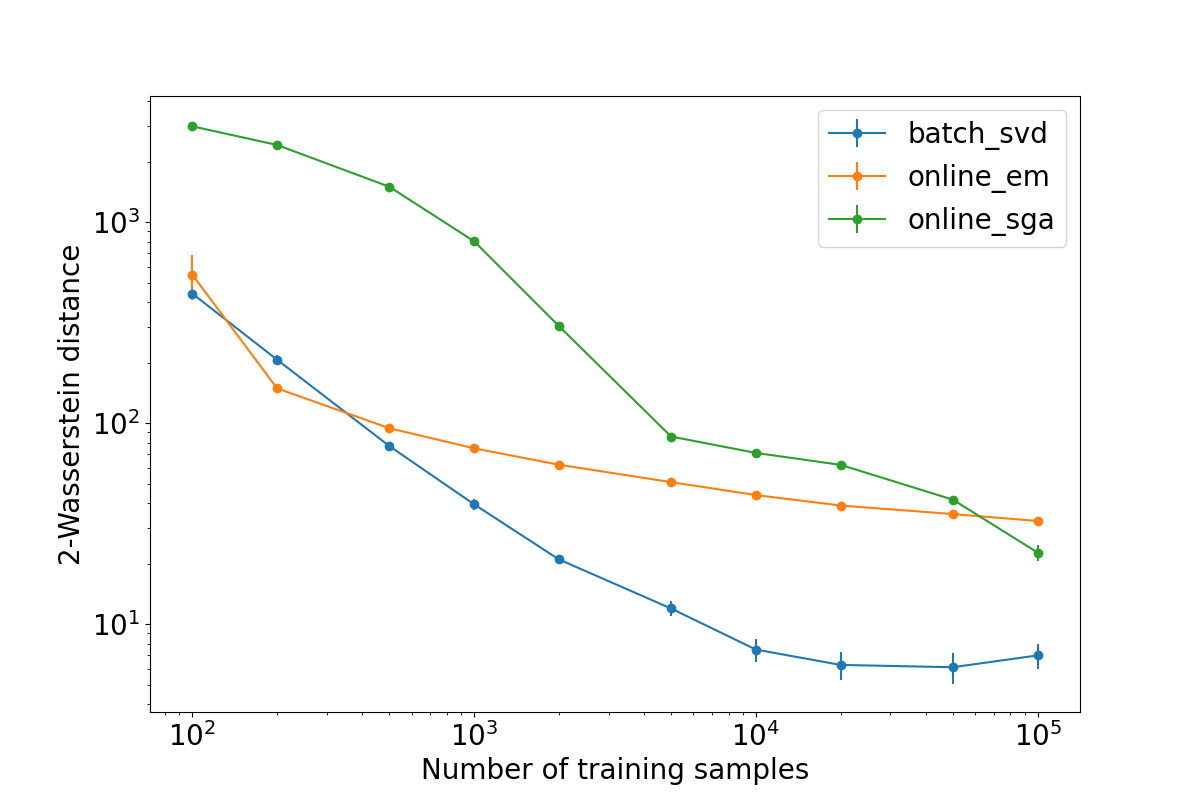
\includegraphics[width=70mm]{plots/online_fa_wasserstein__observation_dim=100__latent_dim=10__spectrum_min=1__spectrum_max=100.png} 
		 & 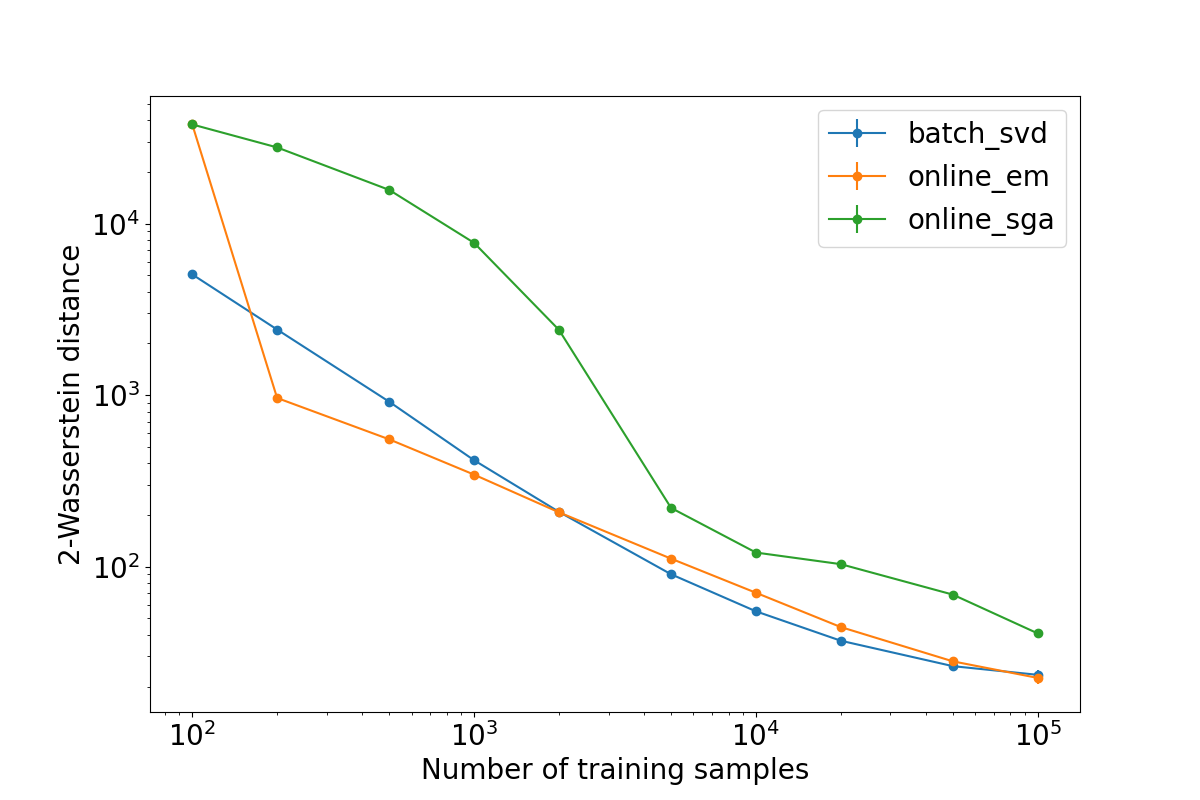
\includegraphics[width=70mm]{plots/online_fa_wasserstein__observation_dim=1000__latent_dim=10__spectrum_min=1__spectrum_max=100.png} \\
		 (c) $D=100$, $K=10$, $\matr{s}^2 \sim \mathcal{U}(1, 100)$ 
		 & (d) $D=1000$, $K=10$, $\matr{s}^2 \sim \mathcal{U}(1, 100)$\\[6pt]
		 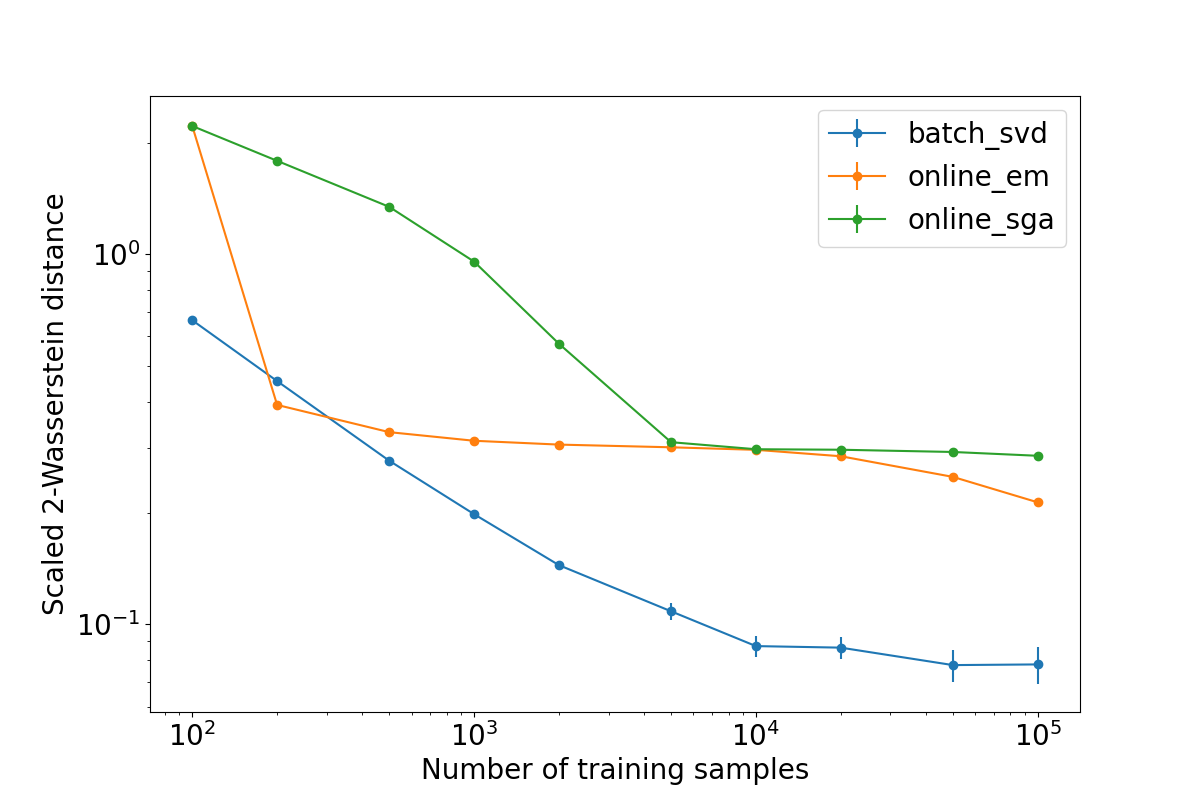
\includegraphics[width=70mm]{plots/online_fa_wasserstein__observation_dim=100__latent_dim=10__spectrum_min=1__spectrum_max=1000.png} 
		 & 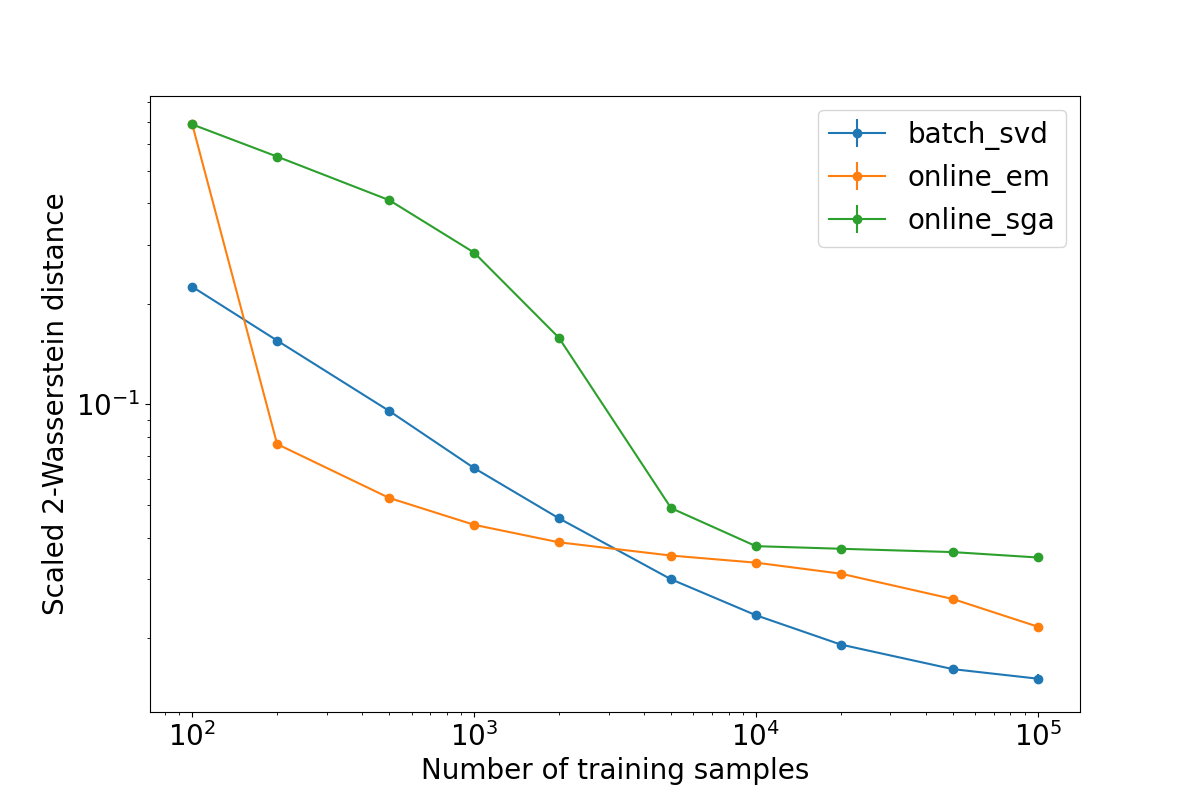
\includegraphics[width=70mm]{plots/online_fa_wasserstein__observation_dim=1000__latent_dim=10__spectrum_min=1__spectrum_max=1000.png} \\
		 (e) $D=100$, $K=10$, $\matr{s}^2 \sim \mathcal{U}(1, 1000)$ 
		 & (f) $D=1000$, $K=10$, $\matr{s}^2 \sim \mathcal{U}(1, 1000)$\\[6pt]
	\end{tabular}
	\caption{The 2-Wasserstein distance between the Gaussian distribution defined by each estimated FA model and the Gaussian distribution defined by the true FA model, divided by the observation dimension. The blue, orange and green lines show the scaled 2-Wasserstein distance corresponding to batch SVD, online EM and online SGA, respectively. Each data point shows the mean value over ten trials with different random seeds, and standard error bars are also plotted. The different plots correspond to different combinations of the observation dimension $D$, the latent dimension $K$ and the range of the spectrum $\matr{s}^2$.}
	\label{fig:fa_wasserstein}
\end{figure}

\begin{table}[h!]
	\begin{center}
		\begin{tabular}{|| p{0.12\linewidth} p{0.20\linewidth} p{0.20\linewidth} p{0.20\linewidth} p{0.20\linewidth} ||} 
 			\hline
 			Obs. Dim & Spectrum Range & Batch SVD & Online EM & Online SGA \\ [0.5ex] 
 			\hline\hline
			100 	& $[1, 10]$ 	& $0.0061 \pm 0.0009$ 	& $0.0058 \pm 0.0006$ 	& $0.0062 \pm 0.0004$ \\ 
				& $[1, 100]$ 	& $0.0256 \pm 0.0022$ 	& $0.0246 \pm 0.0021$ 	& $0.0446 \pm 0.0018$ \\ 
				& $[1, 1000]$	& $0.0780 \pm 0.0089$ 	& $0.2137 \pm 0.0054$ 	& $0.2855 \pm 0.0040$ \\ 
			\hline
			1000	& $[1, 10]$ 	& $0.0015 \pm 0.0001$ 	& $0.0016 \pm 0.0001$ 	& $0.0023 \pm 0.0001$ \\ 
				& $[1, 100]$ 	& $0.0048 \pm 0.0002$ 	& $0.0049 \pm 0.0002$ 	& $0.0062 \pm 0.0001$ \\ 
				& $[1, 1000]$ 	& $0.0152 \pm 0.0005$ 	& $0.0217 \pm 0.0003$ 	& $0.0349 \pm 0.0006$ \\ [1ex] 
			\hline
		\end{tabular}
		\caption{The 2-Wasserstein distance between the Gaussian distribution defined by the estimated FA model and the Gaussian distribution defined by the true FA model, divided by the observation dimension, when the number of training samples is 100,000. Each result is the mean value over ten trials with different random seeds, along with standard errors. These results correspond to the right-most points in the plots in Figure \ref{fig:fa_wasserstein}.}
		\label{table:fa_wasserstein}
	\end{center}
\end{table}

\section{UCI Linear Regression Posterior Estimation}\label{app:uci_posterior}

This section provides more details and results for the linear regression posterior estimation experiments using VIFA in Section \ref{sec:vifa_posterior_uci}. Recall that four UCI regression datasets were used in these experiments. Table \ref{table:uci_datasets} shows the number of instances and input variables in each UCI regression dataset. Note that the original Energy Efficiency dataset has two target variables, heating load and cooling load, but in these experiments only the heating load was used. 
\begin{table}[h!]
	\begin{center}
		\begin{tabular}{||c c c ||} 
			\hline
 			Dataset & No. of Instances & No. of Input Variables \\ [0.5ex] 
			\hline\hline
			Energy Efficiency 				& 768 	& 8 \\
 			\hline
 			Boston Housing 				& 506 	& 13 \\ 
 			\hline
 			Concrete Compressive Strength 	& 1030 	& 8 \\
 			\hline
 			Yacht Hydrodynamics 			& 308 	& 6 \\ [1ex] 
 			\hline
		\end{tabular}
		\caption{UCI regression datasets used in experiments.}
		\label{table:uci_datasets}
	\end{center}
\end{table}

Table \ref{table:vifa_uci_hyperparameters} shows the hyperparameter values used in the experiments.
\begin{table}[h!]
	\begin{center}
		\begin{tabular}{||c c c c c c c c||} 
			\hline
 			Dataset & $K$ & Epochs & $M$ & $L$ & $\eta$ & $\alpha$ & $\beta$ \\ [0.5ex] 
			\hline\hline
			Energy Efficiency 				& 3 & 25,000 & 100 & 10 	& 0.01 	& 0.0608 & 0.1246 \\ 
 			\hline
			Boston Housing 				& 3 & 25,000 & 100 & 10 	& 0.001 	& 0.2859 & 0.0429 \\
 			\hline
 			Concrete Compressive Strength	& 3 & 20,000 & 100 & 10 	& 0.01 	& 0.0254 & 0.0101 \\
 			\hline
 			Yacht Hydrodynamics 			& 3 & 45,000 & 100 & 10 	& 0.01 	& 0.0291 & 0.0114 \\ [1ex] 
 			\hline
		\end{tabular}
		\caption{VIFA hyperparameters for UCI linear regression experiments.}
		\label{table:vifa_uci_hyperparameters}
	\end{center}
\end{table}

Recall that Section \ref{sec:vifa_posterior_uci} presented qualitative comparisons of the true posterior of a linear regression model and the approximate posterior learned by VIFA for the Boston Housing and Yacht Hydrodynamics datasets. Figure \ref{fig:posterior_energy_efficiency} and Figure \ref{fig:posterior_concrete_strength} show the same comparisons for the Energy Efficiency and Concrete Compressive Strength datasets, respectively. Finally, Table \ref{table:linear_regression_vi_posterior_uci} contains quantitative measures of the difference between the true and estimate posteriors for all four UCI datasets. 

\begin{figure}[!htbp] 
	\begin{tabular}{c}
		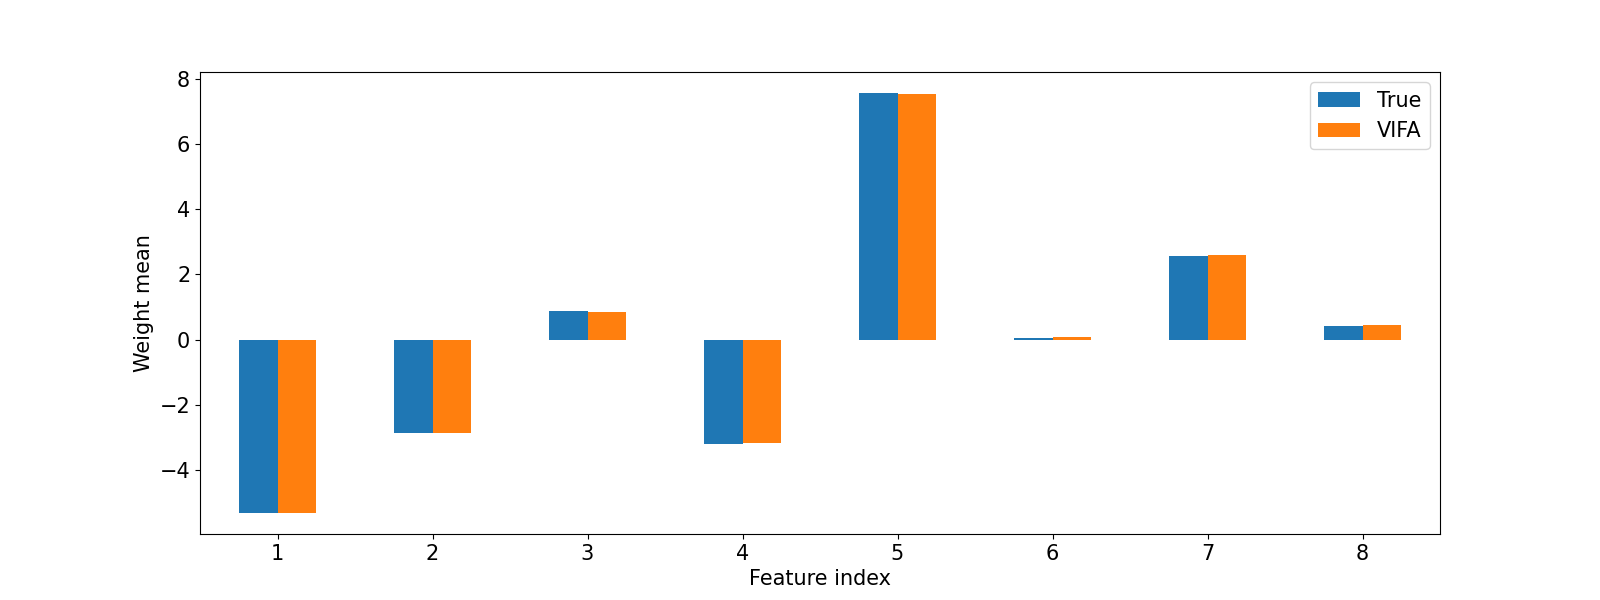
\includegraphics[width=140mm]{plots/energy_efficiency_posterior_mean.png} \\
		(a) Comparison of true and estimated posterior means \\[6pt] 
		 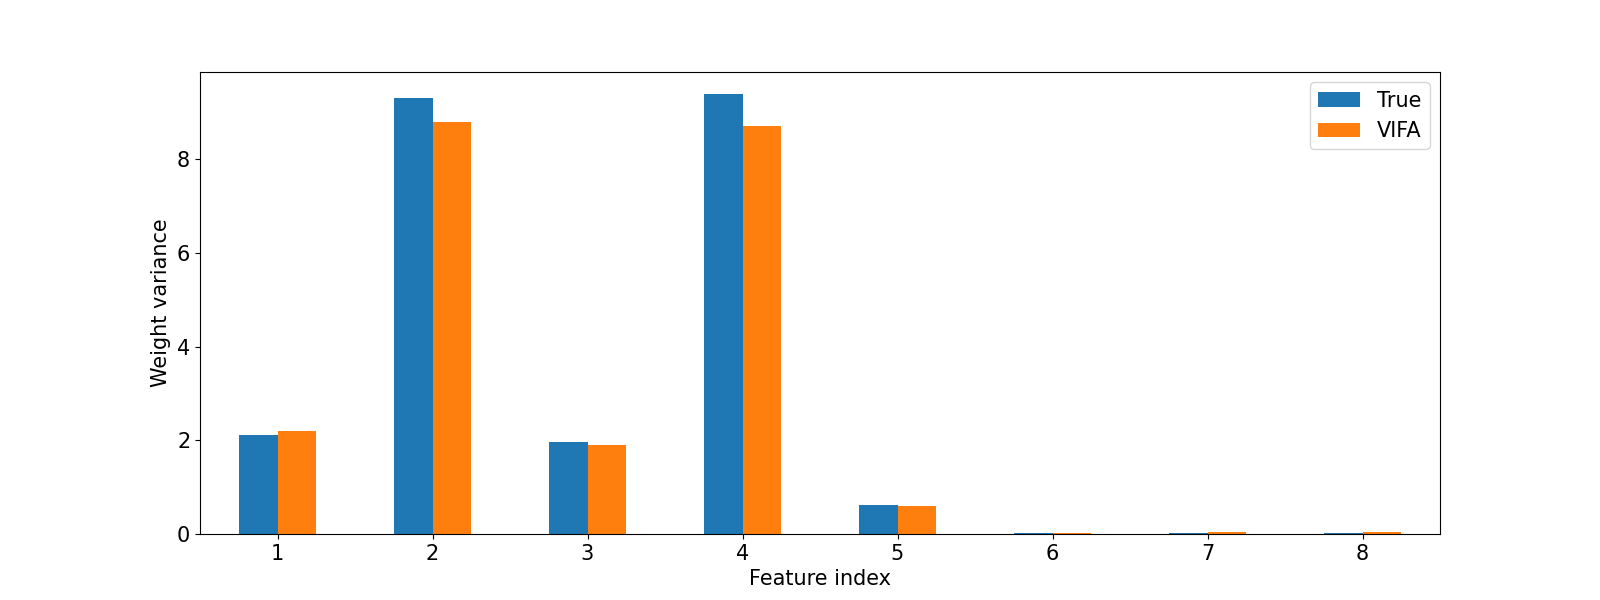
\includegraphics[width=140mm]{plots/energy_efficiency_posterior_variance.png} \\
		(b) Comparison of true and estimated posterior variances \\[6pt] 
		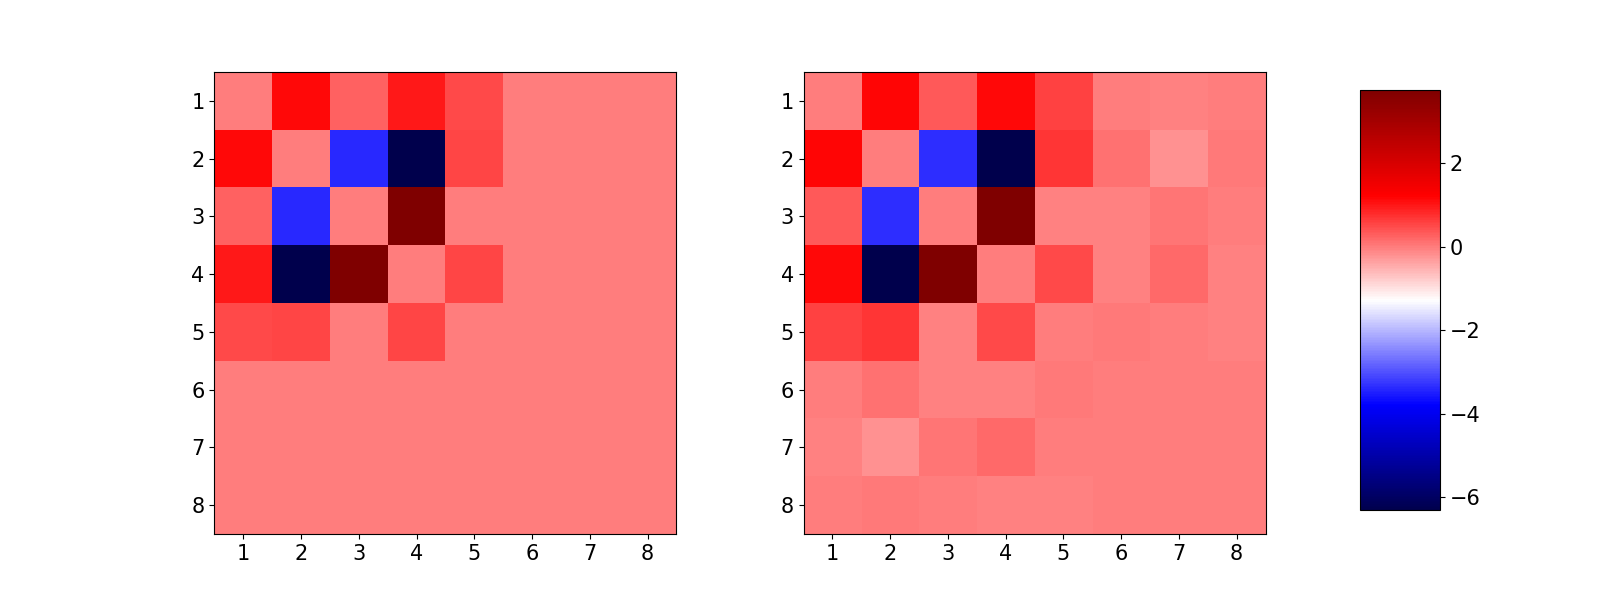
\includegraphics[width=140mm]{plots/energy_efficiency_posterior_covariance.png} \\
		(c) Comparison of true and estimated posterior covariances \\[6pt] 
	\end{tabular}
	\caption{Comparison of the ground truth posterior of a linear regression model fit to the Energy Efficiency dataset, and the approximate posterior learned by VIFA. Variances and covariance are plotted separately due to the difference in their magnitude. In plot (c), the diagonal entries of the covariance matrices have been set to zero.}
	\label{fig:posterior_energy_efficiency}
\end{figure}

\begin{figure}[!htbp] 
	\begin{tabular}{c}
		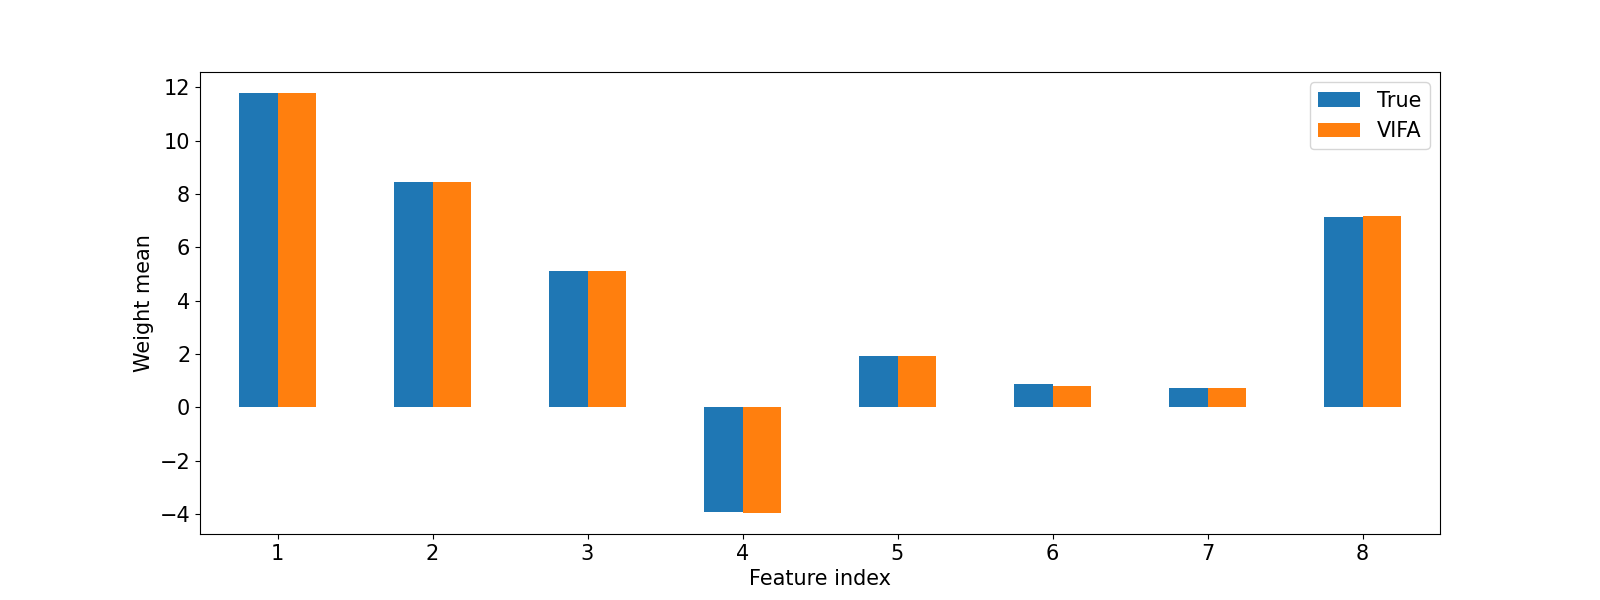
\includegraphics[width=140mm]{plots/concrete_strength_posterior_mean.png} \\
		(a) Comparison of true and estimated posterior means \\[6pt] 
		 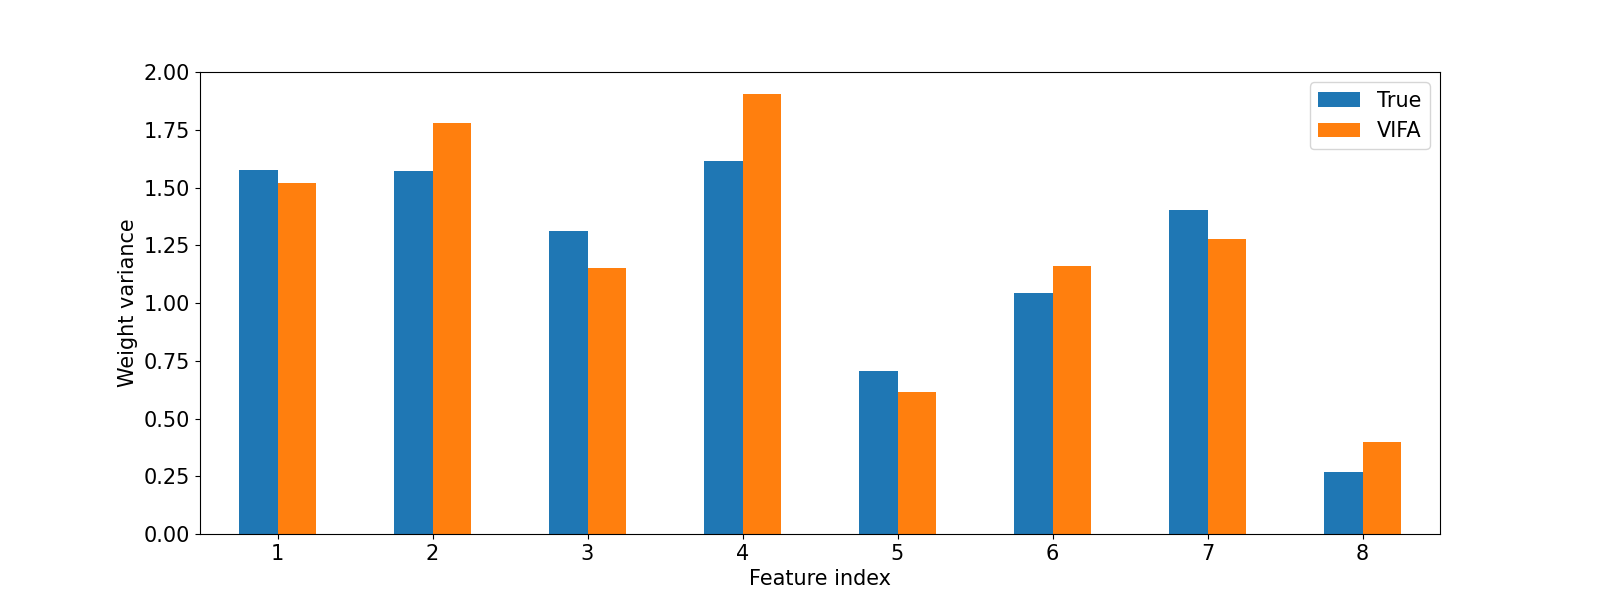
\includegraphics[width=140mm]{plots/concrete_strength_posterior_variance.png} \\
		(b) Comparison of true and estimated posterior variances \\[6pt] 
		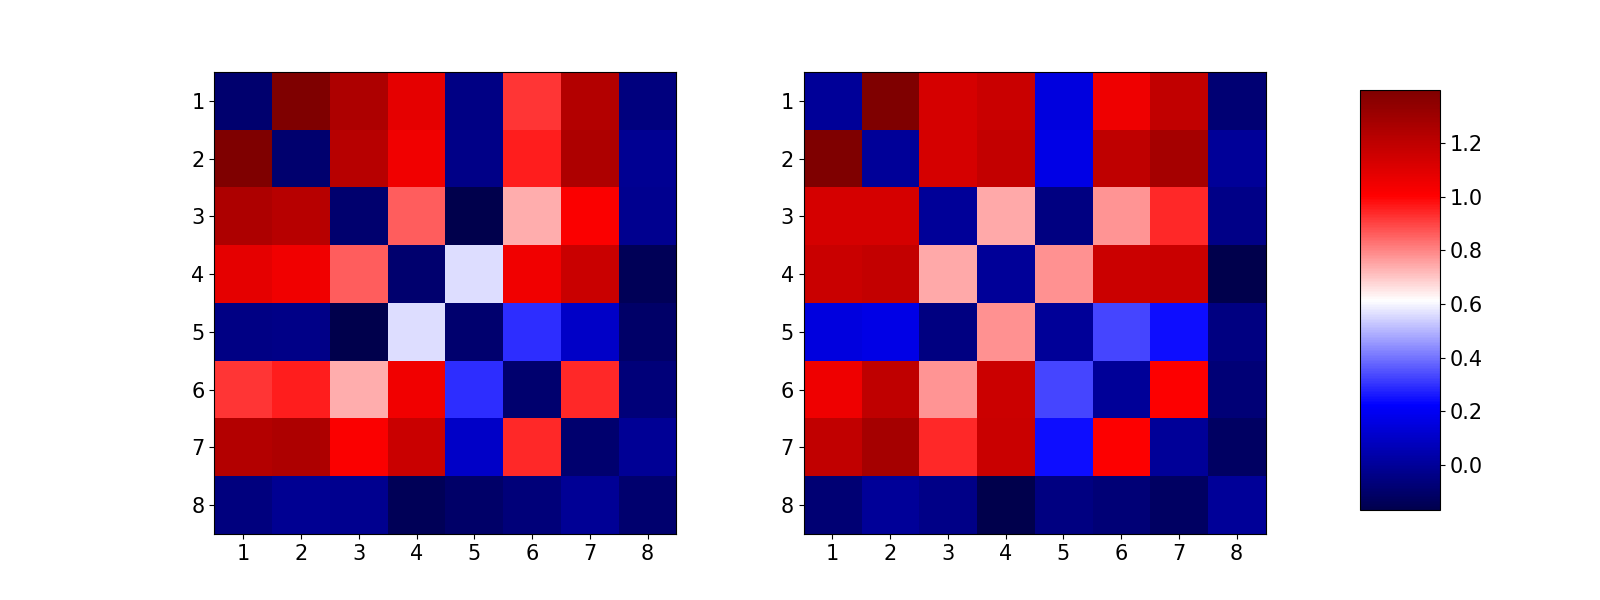
\includegraphics[width=140mm]{plots/concrete_strength_posterior_covariance.png} \\
		(c) Comparison of true and estimated posterior covariances \\[6pt] 
	\end{tabular}
	\caption{Comparison of the ground truth posterior of a linear regression model fit to the Concrete Compressive Strength dataset, and the approximate posterior learned by VIFA. Variances and covariance are plotted separately due to the difference in their magnitude. In plot (c), the diagonal entries of the covariance matrices have been set to zero.}
	\label{fig:posterior_concrete_strength}
\end{figure} 

\begin{table}[h!]
	\begin{center}
		\begin{tabular}{|| p{0.21\linewidth} p{0.21\linewidth} p{0.21\linewidth} p{0.21\linewidth} ||} 
 			\hline
 			Dataset & Relative Distance from Mean & Relative Distance from Covariance & Scaled Wasserstein Distance \\ [0.5ex] 
 			\hline\hline
			Energy Efficiency 	& 0.0051 	& 0.0421 & 0.0564 \\ 
			\hline
			Boston Housing 	& 0.0262 	& 0.3185 & 0.0468 \\ 
			\hline
			Concrete Strength 	& 0.0047 	& 0.0840 & 0.0278 \\ 
			\hline
 			Yacht Hydro. 		& 0.0435 	& 0.0391 & 0.1210 \\ [1ex] 
			\hline
		\end{tabular}
		\caption{For each UCI dataset, the distance between the true posterior distribution of the parameter vector of a linear regression model and the approximate FA posterior estimated by VIFA. Relative distances between the true and approximate means and covariances are shown. Each relative distance is the Frobenius norm of the difference between the true parameter and the approximate parameter divided by the Frobenius norm of the true parameter. Also shown is the 2-Wasserstein distance between the true posterior Gaussian distribution and the approximate Gaussian distribution, divided by the number of dimensions in the dataset.}
		\label{table:linear_regression_vi_posterior_uci}
	\end{center}
\end{table}

\section{UCI Neural Network Predictions}\label{app:uci_nn_predictions}

This section provides more details about the loss functions used in the neural network prediction experiments in Section \ref{sec:uci_nn_predictions}. When training, the average negative log-likelihood term used on line 12 of Algorithm \ref{alg:vi_fa} was set to
\begin{equation}\label{eqn:train_nll}
	-\frac{1}{M} \sum_{(\matr{x}, y) \in \mathcal{B}} \log \mathcal{N}\big(y; f(\matr{x}; \theta), \beta^{-1}\big),
\end{equation}
where $\mathcal{B}$ is a mini-batch of $M$ training examples, $f(\matr{x}; \theta)$ is the prediction of the neural network for input $\matr{x}$ and parameters $\theta$ and $\beta$ is a hyperparameter. 

When testing, the marginal log-likelihood of a test example $(\matr{x}, y)$ is
\begin{align}
\begin{split}
	\log p(y | \matr{x}, \alpha, \beta, \mathcal{D}) 
	& = \log \int p(y | \matr{x}, \theta, \beta) p(\theta | \alpha, \beta, \mathcal{D}) d\theta \\
	& = \log \int \mathcal{N}\big(y; f(\matr{x}; \theta), \beta^{-1}\big) p(\theta | \alpha, \beta, \mathcal{D}) d\theta,
\end{split}
\end{align}
where $\mathcal{D}$ is the training data and $p(\theta | \alpha, \beta, \mathcal{D})$ is the approximate posterior learned by VIFA or SLANG for hyperparameters $\alpha$ and $\beta$. This integral cannot be computed exactly. Instead, it was approximated by a sample average. Formally, 
\begin{align}
\begin{split}
	\log p(y | \matr{x}, \alpha, \beta, \mathcal{D}) 
	& \approx \log \Bigg( \frac{1}{L} \sum_{l=1}^L \mathcal{N}\big(y; f(\matr{x}; \theta_l), \beta^{-1}\big) \Bigg) \\
	& = \log \Bigg( \sum_{l=1}^L \mathcal{N}\big(y; f(\matr{x}; \theta_l), \beta^{-1}\big) \Bigg) - \log L,
\end{split}
\end{align}
where each $\theta_l \sim p(\theta | \alpha, \beta, \mathcal{D})$. This quantity was averaged over the full test set to approximate the average marginal log-likelihood. In addition, the test root mean squared error (RMSE) was also computed, where the squared error of a single test example is
\begin{equation}
	\Bigg(y - \frac{1}{L} \sum_{l=1}^L f(\matr{x}; \theta_l)\Bigg)^2.
\end{equation}
When computing these metrics, the Monte Carlo average size was set to $L=100$.

\end{document}